%\documentclass[a4paper,10pt]{book}
%\usepackage[utf8]{inputenc}
%\usepackage[T1]{fontec}

\documentclass[a4paper,12pt,fleqn,twoside,openany]{book}
\usepackage{layout}
% Set equal margins on book style
\setlength{\voffset}{0pt}
\setlength{\headsep}{25pt}
\setlength{\footskip}{25pt}
\setlength{\oddsidemargin}{0.7in}
\setlength{\evensidemargin}{0pt}
\setlength{\marginparwidth}{10pt}

\usepackage[margin=1in]{geometry}

\geometry{
left=30mm,
right= 20mm}


% Ejemplo página
% \usepackage{geometry}
%  \geometry{
%  a4paper,
%  total={170mm,257mm},
%  left=20mm,
%  top=20mm,
%  }
% 


%\documentclass[a4paper,12pt,oneside,openright]{report}
\usepackage[utf8]{inputenc}
\usepackage[spanish, es-tabla]{babel}
\usepackage{graphicx}
\usepackage{pdfpages}

\usepackage{hyperref}
\hypersetup{
	pdftitle={Diseño, fabricación y caracterización de esponjas psudoelásticas},		% title
	pdfauthor={Lucia Helena Prado},	% author
	pdfsubject={Tesis de Grado},	% subject of the document
    pdfkeywords={Memoria de forma} {Esponjas metalicas} {Cu–Zn–Al},
	colorlinks=true,		% false: boxed links;
	citecolor=black,		% color of links to bibliography
	filecolor=black,		% color of file links
	linkcolor=black,		% color of internal links
	urlcolor=black			% color of external links
}

\usepackage[figure]{hypcap}



% Uso las fuentes iwona para el texto y para matemática.
\usepackage[T1]{fontenc}
\usepackage[math]{iwona}
\linespread{1.05}

%\usepackage{savetrees}

% No se cuales de estos son realmente necesarios.
\usepackage{amssymb}
\usepackage{amsfonts}
\usepackage{amsmath}
\usepackage{multicol}
% Me pone el número de figura en negrita.
\usepackage[bf]{caption}
\usepackage{subcaption}
% Paquete para que las figuras no se vayan al final de los capítulos
\usepackage{afterpage}
\usepackage{color}
% Para tener tablas más lindas
\usepackage{booktabs}
%\newcommand{\ra}[1]{\renewcommand{\arraystretch}{#1}}
\renewcommand{\arraystretch}{1.3}
% \usepackage{biblatex}

% Pongo lindo el header
\usepackage{fancyhdr}
\pagestyle{fancyplain}
\fancyhf{} % clear all header and footer fields
\fancyhead[LE,RO]{\thepage}
\fancyhead[LO]{\slshape \rightmark}
\fancyhead[RE]{\slshape \leftmark}
\fancypagestyle{plain}{% en los inicios de capitulo
	\fancyhead{} % get rid of headers
	\renewcommand{\headrulewidth}{0pt} % and the line
	\fancyfoot[C]{\thepage} % add page number
}

\begin{document}

\begin{titlepage}
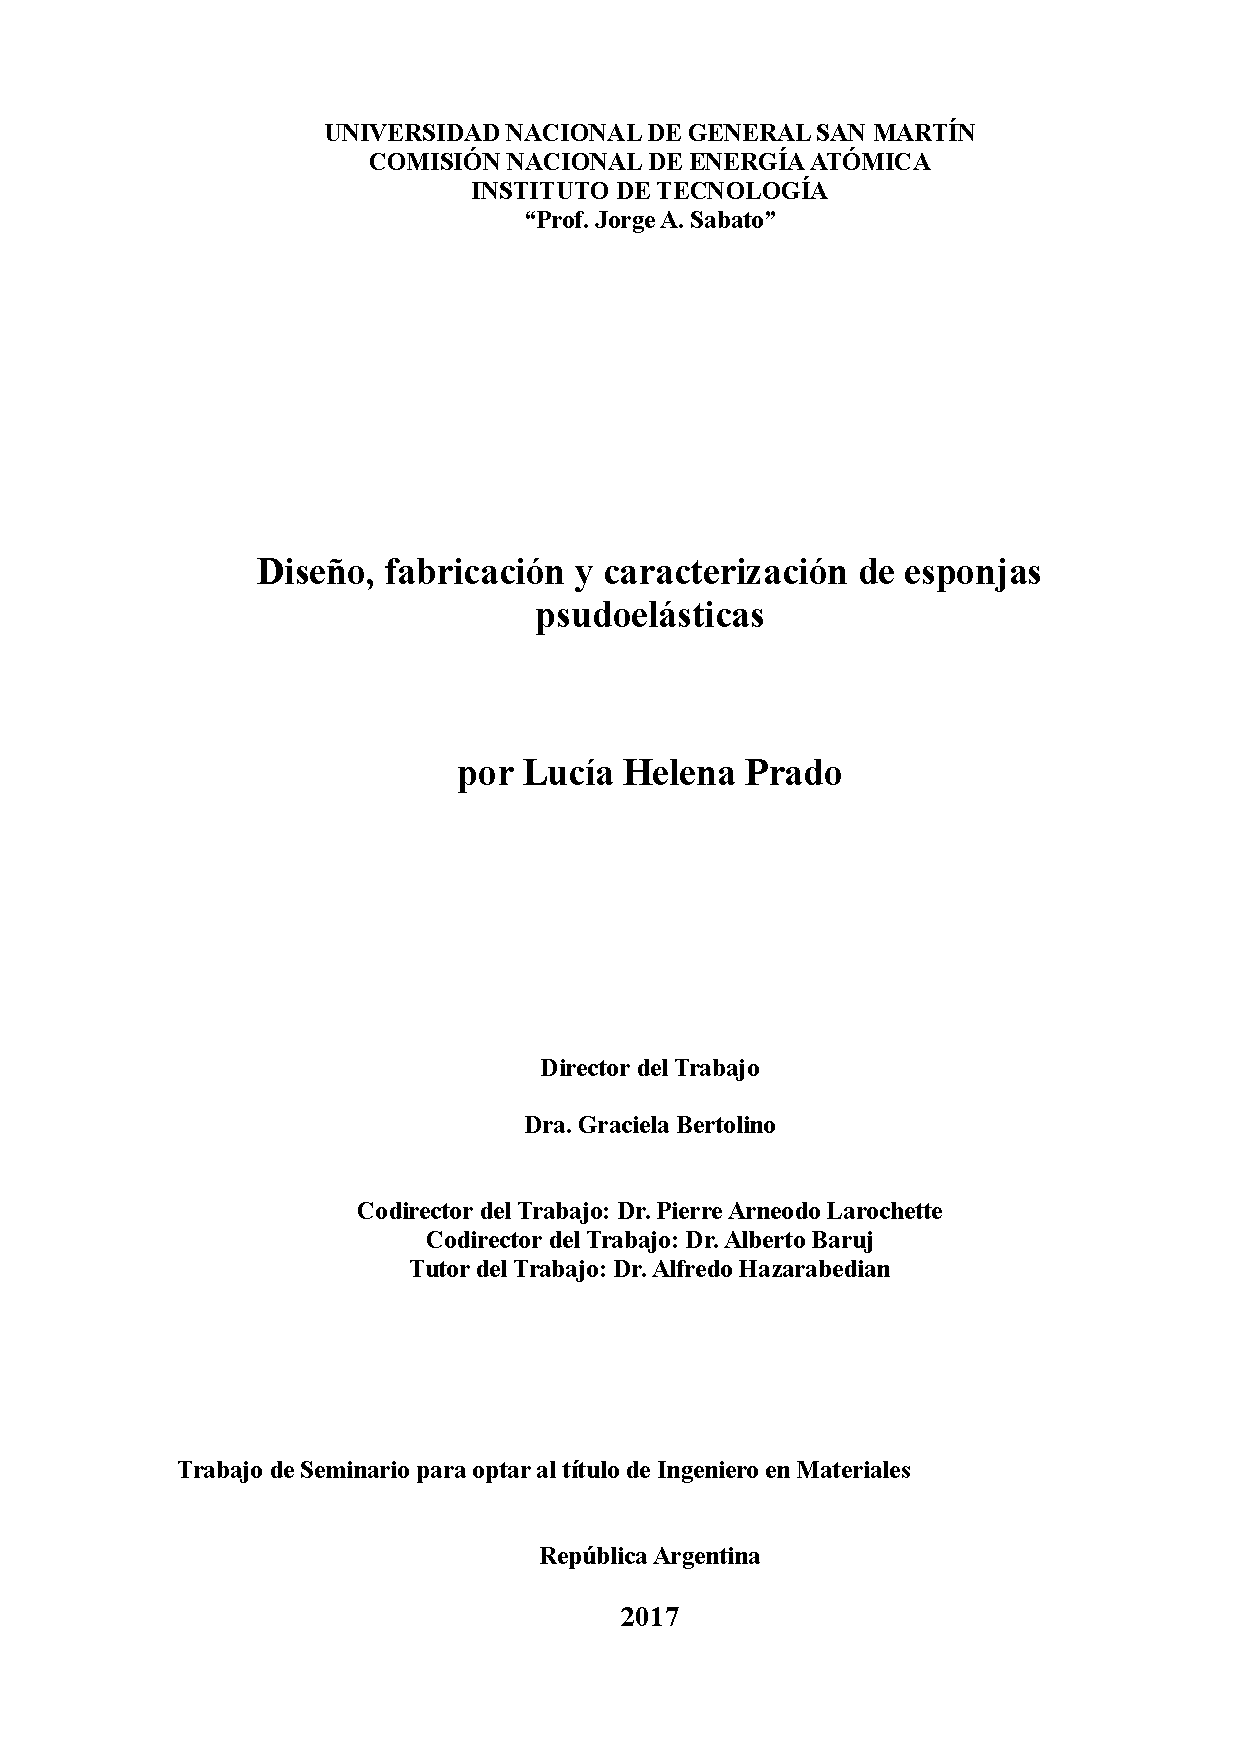
\includepdf[page={-},offset=0mm 0mm]{Img/caratula_is.pdf}
\end{titlepage}

\thispagestyle{empty}
\cleardoublepage

\begin{titlepage}
\begin{flushright}
\large \sffamily

\vspace*{-1.7cm}
% Logo mini de la facultad arriba a la derecha

\includegraphics[width=.2\textwidth]{Img/logo_is.jpg}\\[2cm]
% Logo de la facultad arriba a la izquierda
% \begin{flushleft}
% \includegraphics[width=.6\textwidth]{fiuba.pdf}\\[2cm]
% \end{flushleft}

% Título
\begin{huge}
\bfseries
\textbf{Diseño y caracterización de esponjas pseudoelásticas}\par
\end{huge}
% {\Large \bfseries
% Técnicas de cooperación en redes de sensores: Transmisión cooperativa mediante
% OSTBC}\\
\rule{\linewidth}{1.5mm}\\[0.1cm]
\textsc{Seminario de Ingeniería en Materiales}\\[2.5cm]

% Autor y director
{\small autor:}
Lucía Helena \textsc{Prado}\\

\vspace{10mm}
{\small directora:}
Dra. Graciela \textsc{Bertolino} \\
{\small codirector:}
Dr. Pierre \textsc{Arneodo Larochette} \\
{\small tutor:}
Dr. Alfredo \textsc{Hazarabedian} \\


% Lugar y fecha al final
\begin{table*}[b]
\flushbottom
\centering \sffamily %\scshape \large
\textsc{República Argentina}\\[1mm]
\today
\end{table*}

\end{flushright}
\end{titlepage}

\thispagestyle{empty}
\cleardoublepage

% Agradecimiento
\chapter*{Agradecimientos}

¡\textsc{Gracias Totales}!


% Elimino el header de la página par
\newpage
\thispagestyle{empty}
\cleardoublepage


\tableofcontents

\chapter*{Resumen}

Las aleaciones con memoria de forma han sido objeto de mucho estudio debido a la gran variedad de aplicaciones que presentan como actuadores y amortiguadores. De particular interés resulta la aleación de Cu-Zn-Al que posee buenas características de memoria de forma, y es mucho más simple y económico para trabajar que las aleaciones base titanio utilizadas más comúnmente.
 
Las esponjas metálicas también fueron ampliamente estudiadas ya que poseen muy buenas propiedades mecánicas, como soportar deformaciones mucho mayores y un bajo peso más bajo que los meterial sólidos. Si esto se combina con la capacidad de recuperar su forma inicial al retirar una carga y la absorción de energía debido al efecto pseudoelástico, se obtiene un material capaz de una excelente amortiguación.
 
En este trabajo se desea combinar ambas características, estudiando el desempeño de esponjas metálicas fabricadas a partir de la aleación de Cu-Zn-Al. Para ello se siguieron dos líneas de investigación. En la primera se buscó optimizar el tamaño de grano de la aleación, ya que dicha propiedad impacta directamente las propiedades mecánicas y de memoria de forma del material. Por otro lado, se caracterizó el funcionamiento de esponjas realizadas con esta aleación cuando son utilizadas como amortiguadores. Se prestó particular interés a la posibilidad de determinar el deterioro de las esponjas mediante análisis simples que se puedan hacer sin quitar la pieza de servicio.
 
Los resultados obtenidos muestran que el nivel de deterioro de la estructura de la esponja se puede estimar realizando mediciones de conductividad eléctrica de la misma. En el trabajo se desarrolló un método para discernir la contribución a la variación de las características eléctricas de los diferentes procesos que ocurren durante las deformaciones, que incluyen los cambios por la transformación martensítica y rotura de la estructura.

\chapter*{Summary}

Shape memory alloys are a very active research subject due to the sheer number of possible applications that they can have as actuators or shock absorbers. It’s of special interest the Cu-Zn-Al alloy, as it presents shape memory characteristics while being easier and cheaper to work with than the most commonly used titanium based ones.
 
Metal foams are also very widely studied for their interesting mechanical properties like strain resistance and their low weight. If you combine their capacity to regain their initial shape with their shock absorption properties, they also become a very interesting option for the same applications.
 
In this work we study the characteristics of metal foams that are made out of the Cu-Zn-Al alloy. This work is divided in two major sections. The first one studies mechanisms to control the grain size of the alloy, a critical characteristic for shape memory and mechanical properties which becomes more important when manufacturing foams as the metal will need to be melted twice during the process. The second section consists of a characterization effort done on the shape memory foams when used for shock absorption applications. Special interest was given to methods that can measure the structural damage suffered by the foam while in service.
 
The results show recommendations on how to perform ball milling and use refining additions to achieve the desired grain size while preparing the alloy. We also developed a novel method to determine the mechanical damage of the foam by measuring its electrical conductivity. This method is of particular interest as it can discriminate between variations in the electrical properties due to the martensitic transformations and physical damage, while being simple to use continuously without taking the part out of service.

\chapter{Introducción}

\section*{Objetivo y organización}
Tanto las aleaciones con memoria de forma como las esponjas metálicas son temas que constituyen campos de investigación y desarrollo muy activos actualmente, particularmente por sus aplicaciones como amortiguadores. Resulta de interes combinar las dos propiedades y realizar esponjas a partir de aleaciones con memoria de forma como la aleación Cu–Zn–Al. Estudiar la fabricación y posterior utilización de estas esponjas como elementos amortiguadores son los dos objetivos de este trabajo.

La fabricación de esponjas con memoria de forma es de por sí interante y desafiente. Controlar el tramaño de grano de la aleación es importante para asegurar buenas propiedades de memoria de forma. Sin embargo, el proceso de fabricación de las esponjas involucra múltiples fundiciones, lo que hace que controlar esta propiedad requira especial atención. Por este motivo es que proponer un método para la preparación de la aleación utilizando molienda mecánica y un agente refinador fue el primer objetivo del trabajo.

Una vez fabricada la esponja es necesario tener un entendimiento acabado de los procesos que ocurren cuando son expuestas a reiteradas compresiones, por ejemplo, al estar funcionando como amortiguadores. Durante dichos ciclos se combinan los efectos de la transformación matercítica y las deformaciones de la estructura por las tensiones aplicadas. Entender la contribución de cada uno de ellos a variables fácilmente medibles durante la operación de la pieza es el segundo objetivo de este trabajo.

El trabajo está distribuido en tres capítulos principales. La presente introducción, que senta las bases sobre las cuales se desarrolla el trabajo repasando la transformación martencítica, la aleación Cu–Zn–Al y las esponjas metálicas, entre otros temas fundamentales. En la siguiente sección se detallan los diferentes procedimientos experiemntales que se utilizaron tanto para el desarrollo del método de control de tamaño de grano como para caracterizar las esponjas resultantes.

Los resultados de cada uno de los ejes de este trabajo se detallan en la sección \ref{sec:resultados}. En ella se propone un procedimiento para la fabricación de la aleación donde se utliza molienda mecánica en conjunto con una pequeña cantidad de agente refinador para obtener el tamaño de grano desado y poder preservarlo luego de fundir la aleación para la fabricación de las esponjas.

El segundo resultado de este trabajo es un método que permite estimar el daño estructural por ciclos de compresiones que sufrió una esponja analizando las variaciones en la conductividad eléctrica de la misma. Este método presenta ventajas sobre otras metodologías conocidas, no sólo por la simpliza del equipo requerido, sino, principalmente, al no requerir retirar la pieza de funcionamiento para ser analizada.

\section{Transformación Martensítica}

Las transformaciones de fase se dividen en dos grupos:  con difusión y sin difusión, dependiendo de si hay un movimiento de átomos de largo alcance o no,
respectivamente. Las transformaciones sin difusión también reciben el nombre de displacivas, que a su vez se dividen en transformaciones no macroscópicas
(implican movimientos atómicos menores a un parámetro de red), y macroscópicas (más de un parámetro de red).
La transformación martensítica corresponde a una transformación de fase displaciva en estado sólido. En estas transformaciones se produce un reacomodamiento de los átomos que se mueven cooperativamente distancias menores a un parámetro de red 
por lo que no ocurre difusión de largo alcance. Esto hace que la fase inicial y la fase martensítica tengan la misma composición. 


%\paragraph{}

La fase martensítica se forma por nucleación y crecimiento de placas, las cuales nuclean de forma heterogénea en bordes de grano y defectos de la red. 
Cada placa crece en distintas direcciones, según las tensiones que se generen en la red, hasta alcanzar otro borde de grano o placa de martensita. 
Además, si bien la red sufre una distorsión en cada placa, la suma de todas las distorsiones del material es aproximadamente nula. 
La interfase entre la placa de martensita y la austenita avanza a la velocidad del sonido, lo que hace que la transformación no dependa del 
tiempo, sino únicamente de la temperatura. Esta interfase se llama plano de hábito, pertenece a ambas fases 
simultáneamente y no está distorsionado. Este plano se acomoda por medio de cizalladura o por maclas de la martensita. 
El hecho de que la deformación total del material sea nula no implica que no haya una deformación en la red. En la martensita se ven pequeñas 
deformaciones (menores a un parámetro de red) para que la estructura martensítica pueda acomodarse sin deformar la austenita. 
Duering \cite{duering} muestra una analogía para explicar esto: Si tenemos una pared compuesta de ladrillos, no podemos cambiar la forma de un solo ladrillo. 
Deben deformarse los alrededores o el ladrillo se acomoda a la forma del hueco disponible en la pared.

%\paragraph{}

Las primeras placas de martensita se forman al enfriar rápidamente la fase matriz a la temperatura $M_{s}$ (del inglés \textit{Martensite start}). 
A medida que disminuye la temperatura se van formando nuevas agujas y crecen las ya existentes hasta que se llega a una temperatura 
a la cual ya no se forma martensita, $M_{f}$ (del inglés \textit{Martensite finish}). Esto no significa que la estructura sea completamente martensítica. 
Como la transformación implica una expansión de la red, la formación de varias placas puede dejar la austenita remanente comprimida, 
sin espacio para transformar. También puede ocurrir lo inverso, transformar desde una estructura martensítica a la fase inicial 
por un aumento de la temperatura, pasando las temperaturas $A_{s}$ (\textit{Austenite start}) y $A_{f}$ (\textit{Austenite finish}).

%\paragraph{}
  
%\cite{duering} 

Otra forma de inducir la transformación martensítica es por medio de una tensión mecánica aplicada, es equivalente al calentamiento y enfriamiento pero en 
sentido contrario. Enfriar a una temperatura entre $M_{s}$ y $M_{f}$ es equivalente a aplicar una tensión cada vez mayor, mientras que calentar para revertir la 
transformación equivale a una disminución en la fuerza aplicada. La martensita que se forma por arriba de $M_{s}$ por medio de una 
tensión aplicada recibe el nombre de martensita inducida por tensión (se utilizan las siglas SIM del inglés \textit{Stress Induced Martensite})

  
%\subsection{Memoria de forma}  

Al solicitar mecanicamente un material el mismo se deforma mediante el movimiento de los átomos de la red, esto puede producirse en general por maclado o por deslizamiento de planos. En el maclado el movimiento de los átomos es inferior al parámetro de red mientras que en el deslizamiento los enlaces se rompen para formar nuevos. 
% Como dijimos anteriormente la martensita se acomoda al espacio disponible por maclado o cizalladura. Dependiendo del o de los mecanismos que ocurran se obtendrán 
% distintas morfologías y propiedades. En la transformación por maclado, donde existe una simetría entre la estructura de la fase matriz y la nueva, los cristales 
% están conectados por movimientos menores a un parámetro de red, mientras que en la transformación por deslizamiento (o reconstructiva) ocurre un movimiento 
% infinitesimal de los átomos, y por ende, la rotura y formación de los enlaces atómicos. 
Estos dos mecanismos son utilizados por los aceros, 
elementos puros y estructuras como el CsCl \cite{duering, elliott}. El hecho de romper enlaces y formar nuevos hace que las transformaciones de estos 
elementos sea irreversible. Por otro lado las aleaciones con memoria de forma como Cu-Zn-Al o Cu-Zn-Ti sólo sufren un cambio de forma por maclado, lo que hace que esta deformación sea reversible. Además el plano de hábito en la transformación por maclado tiene mayor movilidad. Esto hace que al aplicar o retirar una tensión (o enfriar o calentar) la interfase se mueva fácilmente a medida que ocurre la transformación a martensita, o retransformación a austenita.

%\setlength\fboxsep{0pt}
%\setlength\fboxrule{0.5pt}
%\includegraphics[scale=0.5]{path3336.png}



%\begin{figure}
%    \centering
%    \includegraphics[width=0.4\textwidth]{path.png}
%    \afterpage{\noindent\includegraphics[width=0.4\textwidth]{path.png}}
%    \caption{Awesome Image}
%    \label{fig:awesome_image}
%\end{figure}






%\cite{duering} 
El avance de la transformación martensítica se puede seguir midiendo diferentes parámetros como la variación de resistencia eléctrica, 
el cambio de longitud o de volumen en función de la temperatura. Otra forma de medir la transformación martensítica de manera precisa es realizando 
una curva de tensión vs deformación, la cual puede verse un esquema en la figura. \ref{fig:TensDefSMAMono}. En la sección marcada con I la curva 
corresponde a la deformación elástica de la aleación. En la sección II, cuando se alcanza una tensión 
suficiente para iniciar la transformación, la pendiente comienza a disminuir debido al movimiento de las interfases de las agujas de martensita. 
Como dijimos, estas interfases son bastante móviles por lo que a medida que transforma, aparece un plateau en la curva de tensión deformación. 
Una vez que la transformación avanza y se encuentran las interfases de las distintas placas o llegan a un borde de grano, su movilidad se reduce y 
comienza la deformación elástica de la martensita, lo cual se ve como un nuevo aumento en la tensión de fluencia, como puede verse en la sección III. 
 Es muy importante caracterizar el rango de tensiones en el que la al y pueden aprovecharse las propiedades de memoria de forma. Una vez que la muestra transformó completamente y se aplican tensiones más altas, las agujas que ya se formaron rotarán y se irán orientando en la dirección de la tensión aplicada. Una vez que se deje de aplicar esta tensión las agujas quedarán con la misma orientación ya que la energía entre las distintas orientaciones es prácticamente igual. 
 


%\textbf{Gráfico tensión vs deformación}
\begin{figure}[h]
 \centering
 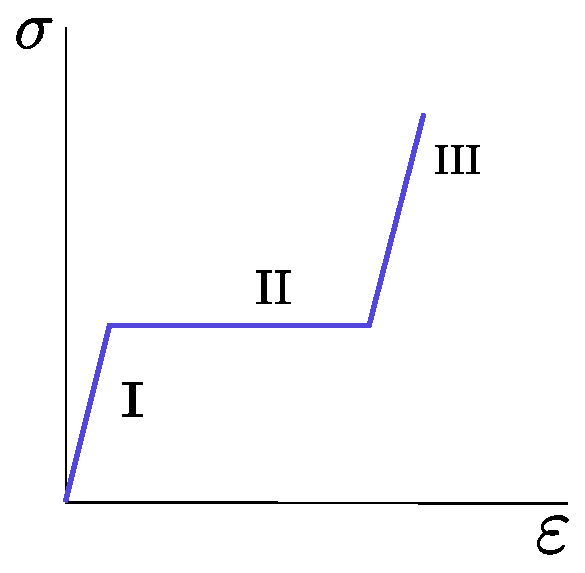
\includegraphics[width=0.4\textwidth]{Img/Introduccion/SigmavsDef.eps}
 \caption{Esquema de una curva tensión vs deformación de un monocristal de una aleación con memoria de forma. Las regiones I, II y III corresponden a las distintas etapas de deformación de la aleación.}
 \label{fig:TensDefSMAMono}
 \end{figure}

 \subsection{Transformación martensítica en monocristales}

Un material con una estructura monocristalina tendrá diferentes direcciones preferenciales para el crecimiento de placas de martensita, por lo que comenzará a transformar cuando la tensión aplicada en una de estas direcciones alcance la tensión crítica. Esta tensión se llama tensión crítica resuelta ($\tau_{R}$) y corresponde a la proyección de la tensión aplicada en las direcciones preferenciales de transformación. Esta tensión resuelta está dada por la Ley de Schmid, en la que si
% Al aplicar una tensión a un material, este transformará y las placas de martensita crecerán en las direcciones preferenciales acomodándose a la dirección de la tensión aplicada. La componente de la tensión aplicada que actúa en la transformación se llama tensión crítica resuelta ($\tau_{R}$) que corresponde a la 
% proyección de la tensión aplicada en las direcciones preferenciales de transformación. Si el material es un monocristal, comenzará a formar las placas de martensita cuando alcance la tensión crítica en alguna dirección preferencial, y todas las placas se formarán siguiendo esta dirección. Las placas crecerán sin necesitar un aumento en la tensión, por lo tanto veremos el plateau en el segmento de transformación. 
%
% Hay que aclarar que la zona II, en la cual ocurre la transformación, no siempre será perfectamente horizontal. Al aplicar una tensión a un material, 
% este se deforma debido al movimiento de dislocaciones en las direcciones compactas de la red cuando esta alcanza la tensión crítica resuelta. La deformación no ocurre 
% en el sentido de la carga aplicada, sino que se deforma en la direcciones compactas. El único caso en que la deformación ocurre en la dirección de la tensión aplicada 
% es cuando ambas coinciden. De esta manera, al aplicar una tensión genérica, la parte que actúa en la deformación se llama tensión crítica resuelta ($\tau_{R}$) que corresponde a la 
% proyección de la tensión aplicada en las direcciones compactas. De manera similar la estructura cristalina tendrá direcciones preferenciales para el crecimiento de las placas de martensita. Si el material es un monocristal, alcanzará la fluencia plástica cuando alcance la tensión crítica en 
% las direcciones compactas de esta configuración, en este caso veremos el plateau en el segmento de transformación. Si en cambio el material es policristalino, cada uno 
% de los granos tendrá una tensión distinta en sus direcciones compactas. Si se va aumentando la carga, primero llegará a la tensión crítica de algunos granos con orientación 
% más favorable y luego alcanzará la tensión crítica en granos con orientaciones menos favorables. Por esto se necesitarán mayores tensiones para deformar un material policristalino.
 se tiene una probeta de 
sección A, y se le aplica un esfuerzo F, la tensión aplicada será:
\begin{equation}
 \sigma = \frac{F}{A}
\end{equation}
Si $\lambda$ es el ángulo entre la tensión aplicada y la dirección de deslizamiento o cizalladura, el esfuerzo cortante efectivo que actúa en este plano será:
\begin{equation}
 F_{R}= F cos(\lambda)
\end{equation}
El área correspondiente al plano donde se ubica la dirección de transformación es:
\begin{equation}
 A_{R}=\frac{A}{cos(\phi)}
\end{equation}
Donde $\phi$ es el ángulo entre la tensión aplicada y la normal al plano de transformación. Por lo anterior, la tensión resuelta que actúa en el plano será:
\begin{equation}
 \tau_{R}=\frac{F_{R}}{A_{R}}= \frac{Fcos(\lambda) }{\frac{A}{cos(\phi)}}=\frac{F}{A} cos(\lambda)cos(\phi) = \sigma cos(\lambda)cos(\phi)
\end{equation}

Cuando la tensión resuelta $\tau_R$ alcanza la tensión crítica de transformación comenzarán a formarse y crecer las placas de martensita.


\subsection{Factores que afectan la tensión crítica de transformación}


Por encima de la $M_s$, la formación de martensita a través de una tensión aplicada sigue un comportamiento lineal \cite{pierre}. Esto es, a mayor temperatura, se 
necesitará una mayor tensión. Por otro lado si se extrapola hasta que la tensión necesaria sea cero se llega a la $M_s$. Este comportamiento se describe con una ecuación 
análoga a la de Clausius-Clapeyron, la cual describe la transformación de una fase a otra:

\begin{equation}
 \frac{dP}{dT}=\frac{\Delta S}{\Delta V}
\end{equation}

Donde P, T, $\Delta$S y $\Delta$V son la presión, la temperatura, el cambio de entropía al transformar y el cambio de volumen, respectivamente. En la línea formada por este gráfico 
coexisten ambas fases. Para la transformación martensítica se utiliza una ecuación equivalente:

\begin{equation}
 \frac{d \tau_{R}}{dT}=\frac{\Delta S}{\Delta V} 
\end{equation}

donde $\tau_{R}$, T, $\Delta S$ y $\Delta V$ son la tensión resuelta, la temperatura, el cambio de entropía y el cambio de volumen respectivamente.




%\begin{figure}
%    \centering
%    \includegraphics[width=0.4\textwidth]{path.png}
%    \afterpage{\noindent 
\includegraphics[width=0.4\textwidth]{clapeyron.png}}
%    \caption{Awesome Image}
%    \label{fig:awesome_image}
%\end{figure}


\begin{figure}[h]
 \centering
 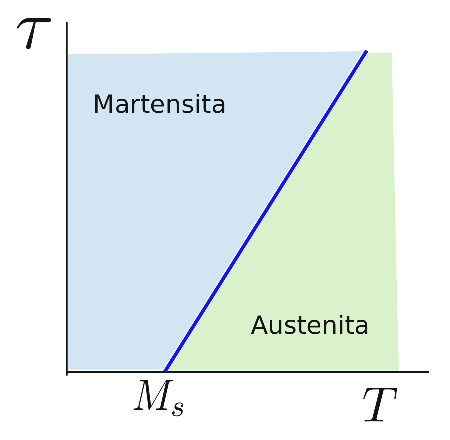
\includegraphics[width=0.4\textwidth]{Img/Introduccion/Clapeyron.eps}
 \caption{Esquema de la variación de la tensión de transformación con la temperatura. Puede verse que cuando la tensión es nula, la temperatura de
 transformación corresponde a la $M_s$}
\end{figure}



%\textbf{Gráfico tensión vs T}



Por encima de $M_s$ y aplicando una tensión, a medida que avanza la transformación, su avance de hace más dificultoso. Al superar una determinada temperatura, la tensión necesaria para 
formar martensita es mayor a la necesaria para mover las dislocaciones. La temperatura a la cual ocurre esto es la $M_d$, y es la mayor temperatura a la cual se puede 
obtener martensita aplicando una tensión. Por este motivo las aleaciones con memoria de forma a partir de la formación de SIM, se utilizan en el rango entre $M_s$ y $M_d$.
Para las aleaciones de Cu-Zn-Al, a $T > 50K$, $\Delta S$ es prácticamente independiente de la temperatura \cite{pierre}, por lo que consideramos que tiene un comportamiento 
prácticamente lineal. Puede verse que cuando no hay tensiones aplicadas la temperatura de transformación coincide con la $M_s$.

\subsection{Transformación martensítica en policristales}
Hay que aclarar que la zona II, en la cual ocurre la transformación, no siempre será perfectamente horizontal. 
Si en cambio el material es policristalino, cada uno de los granos tendrá una orientación distinta, y cada grano alcanzará la tensión crítica resuelta para distintas tensiones aplicadas. Los granos con orientación más favorable transformarán cuando la tensión aplicada alcance la tensión crítica, mientras que los granos orientados menos favorablemente necesitarán tensiones más altas para que la tensión resuelta alcance la tensión crítica de transformación. Por esto se necesitarán mayores tensiones para deformar un material policristalino y además no se encuentra un plató horizontal, sino que presenta una pendiente positiva.


\section{Pseudoelasticidad}

Al graficar la fracción martensítica en función de la tensión aplicada, puede verse que presenta una histéresis, por lo que al transformar y 
retransformar en sentido inverso, la curva no “sigue un mismo camino”. El proceso de transformación martensítica es termoelástico, es decir, la transformación 
no se da únicamente por una fuerza impulsora química, sino que se almacena y libera energía elástica. A medida que avanza la transformación con tensiones aplicadas, 
se almacena energía elástica al transformar y se libera al retransformar en sentido inverso. 

Otras causas que generan la pérdida de energía son la fricción que produce el 
movimiento de interfases y la creación de defectos. El área encerrada en la curva es la energía consumida en un ciclo de transformación y retransformación dándole a los 
materiales con memoria de forma la propiedad de amortiguación.


% Otras causas del almacenamiento de energía elástica son la fricción que produce el 
% movimiento de interfaces y la creación de defectos. El área encerrada en la curva es la energía consumida en un ciclo de transformación y retransformación dándole a los 
% materiales con memoria de forma la propiedad de amortiguadores.


 
 \begin{figure}[h]
 \centering
    \begin{subfigure}{0.49\textwidth}
        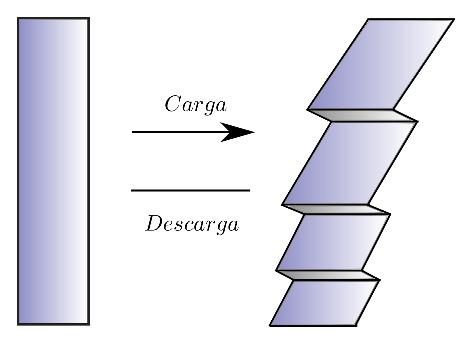
\includegraphics[width=\textwidth]{Img/Introduccion/HisteresisEsquema.eps}
        \caption{}
        \label{fig:}
    \end{subfigure}
    \begin{subfigure}{0.45\textwidth}
        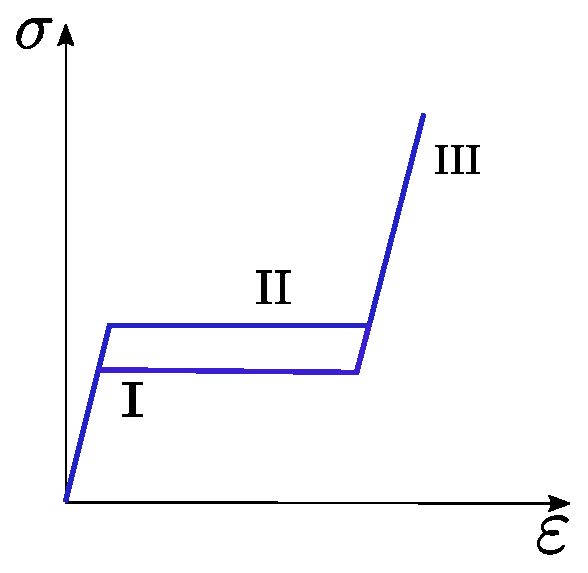
\includegraphics[width=\textwidth]{Img/Introduccion/Histeresis.eps}
        \caption{}
        \label{fig:EspA}
    \end{subfigure}

  \label{fig: proceso}
  \caption{A la izquierda esquema de un material que transforma y vuelve al estado inicial al aplicar y retirar una carga respectivamente.
  A la derecha mismo esquema de transformación donde puede verse la energía consumida al realizar un ciclo de carga y descarga.}
\end{figure}
 
 
Stoiber \cite{stoiber} atribuye el gasto de energía en la transformación a los siguientes fenómenos:
\begin{itemize}
 \item[$\circ$] Procesos de nucleación
 \item[$\circ$] Procesos de no equilibrio inducidos por esfuerzos externos (temperatura o tensiones) que actúan como fuerza impulsora para la 
 transformación
 \item[$\circ$] Contribuciones irreversibles como trabajo de fricción para mover interfases
 \item[$\circ$] Envejecimiento y estabilización de fases (por ejemplo a altas temperaturas) 
\end{itemize}

% La histéresis puede verse en la zona de transformación donde se consume y se libera energía al transformar y retransformar respectivamente. 
% También se ve en la zona donde ya se transformó a martensita y se consume energía en el movimiento de interfases entre martensita y austenita (planos de hábito). 


\section{Memoria de forma}

 Al enfriar una muestra de austenita a una temperatura inferior a $M_{f}$ la muestra transformará a martensita. Por otro lado al calentarla a una temperatura mayor a $A_{f}$ volverá a transformar a austenita. 
 
 Al transformar térmicamente las placas se formarán en distintas direcciones, según las orientaciones que sean más favorables en el material. Si está muestra transformada se deforma manteniendo la temperatura por debajo de $M_s$, las placas se irán orientando (algunas crecen y otras se achican) según la tensión aplicada. Finalmente si se se calienta por encima de $A_{f}$, recuperará su forma original a medida que transforma a austenita. Si luego se enfría nuevamente no habrá un cambio de forma. Este efecto se llama “memoria de forma” ya que ocurre una sola vez, a menos que se vuelva a deformar la muestra en la fase martensítica. La figura \ref{fig:memoria} muestra un esquema de este comportamiento. Existe otra propiedad llamada memoria de forma doble en la que la muestra al 
enfriarse desde austenita a martensita recuperará el estado inicial de deformación. Este comportamiento es mucho más complejo y no se tratará en este trabajo.


\begin{figure}[h]
 \centering
 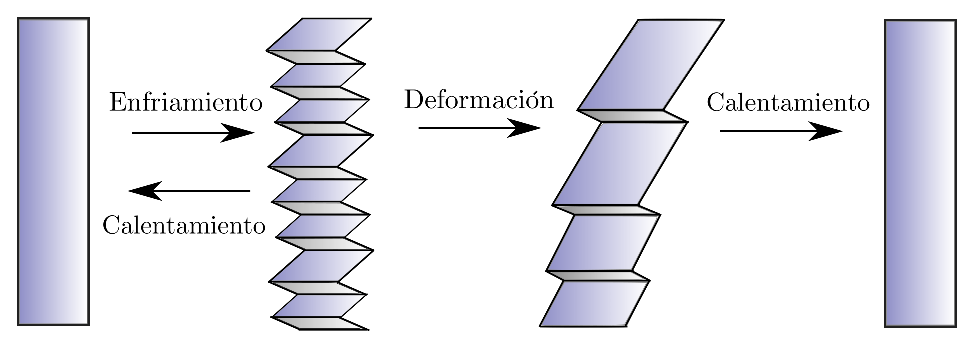
\includegraphics[width=0.8\textwidth]{memoria.eps}
 \caption{Esquema del efecto de memoria de forma. Al enfriar la probeta pasa a estado martensítico. Si luego se deforma y posteriormente se calienta
 la estructura vuelve a su forma inicial.} 
 \label{fig:memoria}
 \end{figure}

%Al enfriar la austenita puede transformar formando agujas de martensita con orientaciones distintas. 

El efecto de memoria de forma se basa en que la 
austenita tiene mayor cantidad de simetrías que la martensita. Así la austenita puede transformar de distintas formas a martensita, pero existe sólo 
una forma en que la martensita transforma a austenita. Esto hace que al retransformar desde la martensita deformada a austenita recupere su forma 
original.

Si la transformación se produce térmicamente, se van formando muchas variantes de martensita en distintas 
direcciones, acomodándose a las tensiones y al espacio disponible en la red. Cuando se producen por una tensión aplicada, las agujas se forman en la dirección de mayor tensión resuelta. Así todas las agujas de martensita quedan alineadas en la misma dirección. Esto hace que al calentar y 
transformar a austenita todo se mueva en la misma dirección y recupere la forma original. Puede ocurrir que se formen dos placas en distinta dirección 
y se crucen, esto hace que en el punto donde se crucen queden ancladas, análogo a lo que ocurre con las dislocaciones, haciendo que las interfases de las placas pierdan movilidad. Un efecto similar se da por el envejecimiento y estabilización de la martensita. Estos son efectos que van en detrimento de las propiedades de memoria de forma.


\section{Aleación Cu-Zn-Al}


\begin{figure}[h]
 \centering
 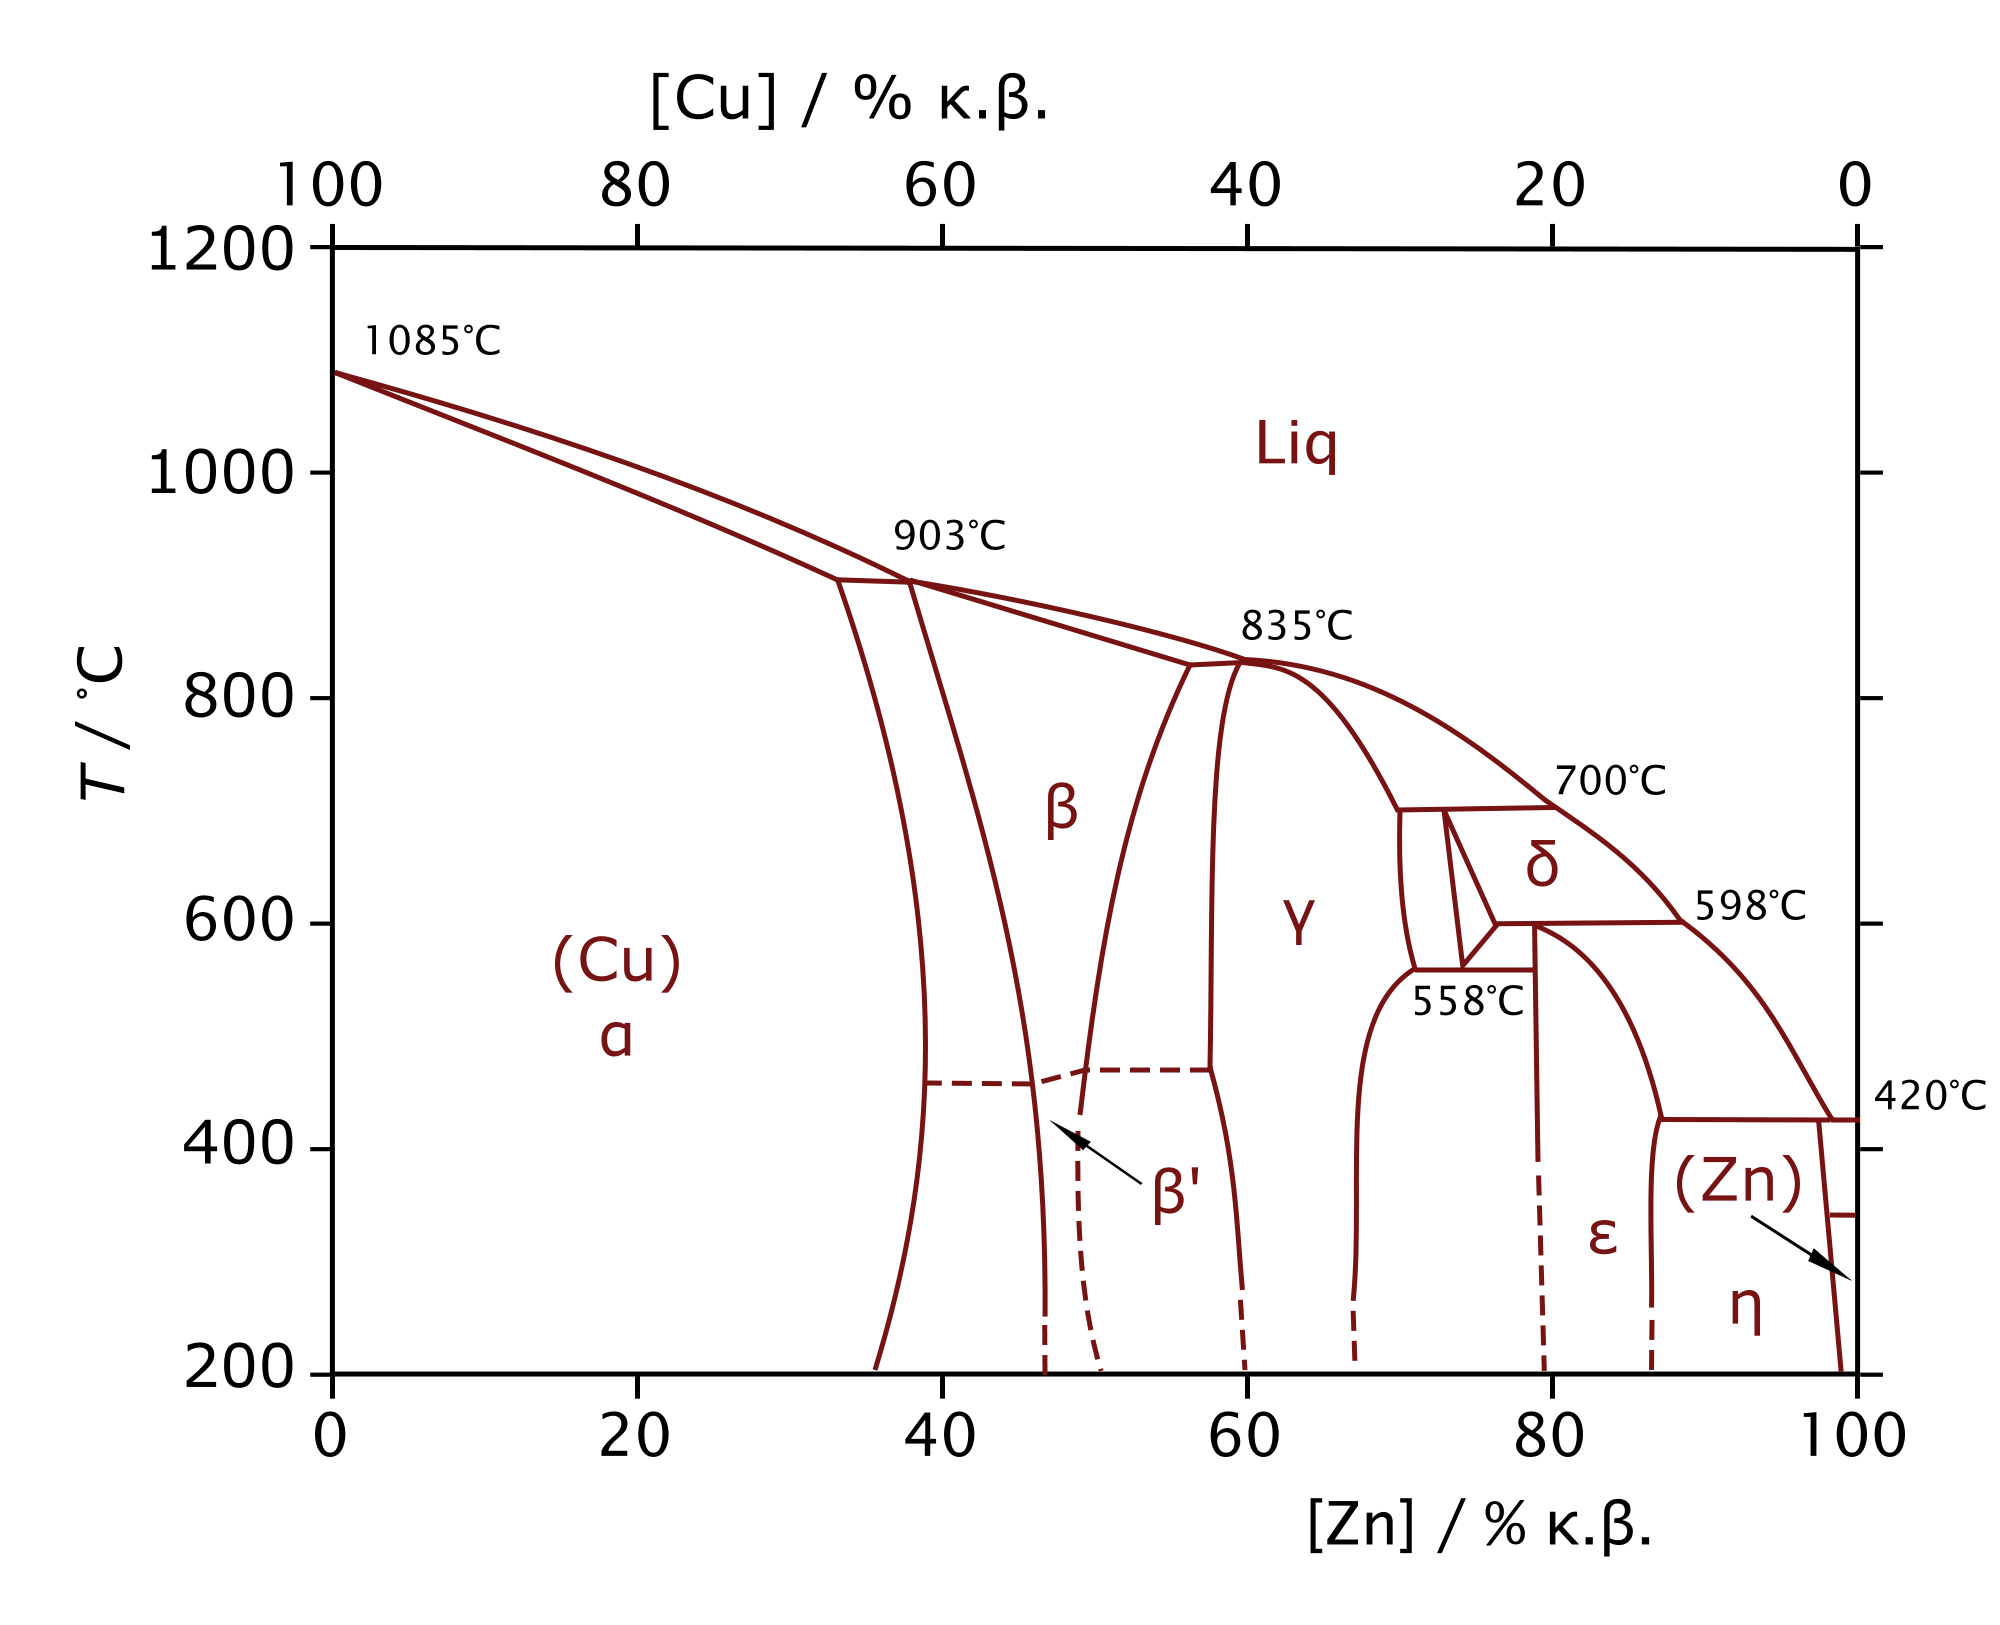
\includegraphics[width=0.8\textwidth]{CuZn.png}
 \caption{Diagrama de equilibrio Cu-Zn \cite{CuZn}} 
 \label{fig:CuZnfig}
 \end{figure}

%  TODO ver si va esto
% En la figura \ref{fig:CuZn} se muestra el diagrama de equilibrio Cu-Zn, y puede verse que si se comienza con una fase $\beta$ y se enfría lo 
% suficientemente lento para permitir difusión, ocurre descomposición de la fase inicial, obteniéndose dos fases estables $\alpha$ y $\gamma$. 
% Para obtener una transformación martensítica, hay que retener la fase $\beta$, que luego puede transformar a martensita con enfriamientos o alicando tensiones $????$. 
En el diagrama de fases estables de la aleación Cu-Zn pueden verse las distintas fases $\alpha$, $\beta$, $\gamma$ y otras más complejas. La fase que nos interesa es la $\beta$, estable a alta temperatura y con una concentración electrónica de 1.48, la cual posee una estructura BCC de tipo A2, esto es, 
los átomos se encuentran desordenados ocupando cualquier posición de la red. La concentración electrónica es otra forma de describir la composición de una aleación, y esta asociado al número de electrones de conducción por átomo en la red. En las aleaciones base cobre cada elemento aporta una cantidad distintas de electrones, y se llega a la concentración electrónica a partir de la siguiente fórmula:

\begin{equation}
\frac{e}{a} = 1+C_{Zn}+2C_{Al}
\end{equation}
donde $C_{x}$ es la concentración atómica de cada elemento y va desde cero hasta uno. 
Siguiendo el gráfico de equilibrio de la Figura \ref{fig:CuZnfig} si se realiza 
un enfriamiento lento la fase $\beta$ se descompone en dos fases de equilibrio $\alpha$ y $\gamma$. Si se realiza un enfriamiento rápido los átomos sufren un ordenamiento de primeros vecinos, esto es, continúan con una estructura bcc pero los átomos ocupan las posiciones similares a una red de CsCl (estructura B2).Finalmente ocurre un ordenamiento a segundos vecinos llegando a un ordenamiento de tipo $L2_1$. Las estructuras martensíticas de la aleación Cu-Zn-Al 
poseen estructuras muy complejas llamadas Long Period Stacking Order (LPSO). Dependiendo de la secuencia de apilamiento de planos 
compactos se obtendrán distintos tipos de martensita. La secuencia de planos compactos que compone la martensita depende de la composición de la 
aleación. Por ejemplo, si se parte de la fase $\beta$ $L2_1$ se llega a una estructura martensítica 18R, en cambio si se parte de una estructura B2 se 
obtendrá un apilamiento de 9 planos compactos llamado 9R. La fase de nuestro interés para obtener una aleación con propiedades de memoria de forma 
es la 18R, la cual puede formar en la transformación $\beta \dashrightarrow 18R$ veinticuatro variantes martensíticas dependiendo del orden de apilamiento 
de los planos compactos. No entraremos en detalle respecto de la estructura de las fases, sino que se presentan de manera ilustrativa.



La aleación de Cu-Zn-Al es muy susceptible a cambios de composición, por ende un cambio muy pequeño en la cantidad de un aleante puede cambiar en gran medida la $M_s$. 
Como se ve en el diagrama estable Cu Zn, a altas temperaturas y con una composición electrónica e/a de alrededor de 1.48 la aleación se compone de una fase $\beta$ (bcc). 
% La concentración electrónica de nuestra aleación está dada por la expresión:
% \begin{equation}
%  \frac{e}{a} = 1+C_{Zn}+2C_{Al}
% \end{equation}

La $M_{s}$ también puede escribirse en función de las concentraciones, existen 
distintas fórmulas empíricas que pueden usarse. Para una concentración electrónica de $\frac{e}{a}=1.48$ la que mejor ajusta es la siguiente:

\begin{equation}
M_s[K]=2686-6400C_{Zn}-9000C_{Al} \label{Ms} 
\end{equation}
Si además usamos que:
\begin{equation}
     C_{Cu}+C_{Zn}+C_{Al}=1
\end{equation}
podemos obtener las concentraciones necesarias para una determinada $M_{s}$. Esto es muy útil ya que buscamos tener una $M_{s}$ menor a la temperatura ambiente, para 
luego poder deformar y obtener un comportamiento pseudoelástico a temperatura ambiente. Si la $M_{s}$ es mayor, la muestra deberá deformarse a mayor temperatura, lo 
cual exige la utilización de un equipo más complejo capaz de controlar simultáneamente tensiones y temperatura.



En el gráfico \ref{fig:mstab} puede verse como una leve variación en el contenido de distintos aleantes cambia muy marcadamente la $M_s$. Además hay que 
tener en cuenta que al fundir la aleación, el Zn se volatiliza y se pierde fácilmente, lo que como dijimos genera un gran cambio en la $M_s$. Esto 
puede contrarrestarse agregando una cantidad de Zn extra para compensar el que se perderá en la fundición.

% \begin{table} 
% \begin{center}
% \begin{tabular}{@{}llll@{}}  \toprule
% $Cu (g)$ & $Zn (g)$ & $Al (g)$ & $M_s$ ($C^\circ$)\\ \midrule
% 12.53 & 2.81  & 1.287 & -34.08\\
% 12.53 & 2.53 ($-10 \%$) & 1.287 & 25.97\\
% 12.53 & 2.38 ($-15 \%$) & 1.287 & 87.87\\
% 12.53 & 1.61 & 1.287 & 285.6 \\
% \bottomrule
% \end{tabular}
% \caption{En esta tabla se muestra como la variación de pequeñas cantidades de Zn puede generar grandes cambios en la $M_s$. Los datos se obtuvieron utilizando la fórmula \ref{Ms}}
% \label{tab:mstab}
% \end{center}
% \end{table}


\begin{figure}[h]
 \centering
 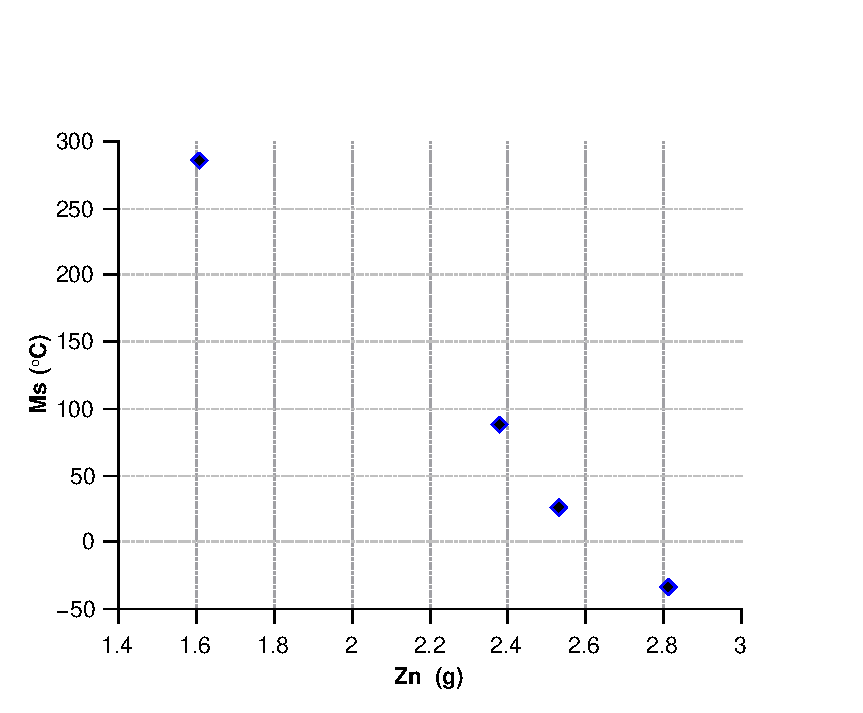
\includegraphics[width=0.6\textwidth]{Img/Introduccion/MsZn2.eps}
 \caption{En este gráfico se muestra la variación de la $M_s$ al variar en pequeñas cantidades la concentración de Zn a partir de la ecuación \ref{Ms}. Las cantidades de Cu y Zn son $12.53 g$ y $1.18 g$ respectivamente.}
 \label{fig:mstab}
\end{figure}


Además de la composición, las temperaturas de transformación varían dependiendo de la historia térmica que sufrió la aleación, ya que influye en la estabilización 
de las distintas fases. Por ejemplo en un austenizado (fase $\beta$) a mayor temperatura se produce un mayor crecimiento de granos, lo que lleva a un aumento en las 
temperaturas de transformación (Hall-Petch). Otro factor importante es el envejecimiento y estabilización de la martensita. Puede ocurrir incluso a temperatura ambiente y generalmente se considera que a partir de $120$ $^\circ C $ la martensita comienza 
a estabilizarse, ocurre un reordenamiento atómico disminuyendo su energía libre y por lo tanto se modifican las temperaturas y tensiones de transformación ($A_s$ y $A_f$ aumentan). Como la estabilización 
de las fases se produce por difusión, los parámetros que la controlan son la temperatura, tensiones aplicadas y la concentración de vacancias. Queda claro que las 
primeras dos variables pueden controlarse fácilmente, mientras que para la concentración de vacancias es más complejo.


% ************************************************* refinar tamaño de grano*************************
A altas temperaturas, donde se encuentra el campo de la fase $\beta$, la aleación presenta un rápido crecimiento de grano. Las interfaces son frágiles y propensas 
a falla por fisuras intergranulares. En la bibliografía pueden encontrarse distintos elementos que actúan como refinadores de grano. Generalmente actúan formando 
precipitados que facilitan la nucleación heterogénea y dificultan el crecimiento de grano. Es por esto que no generan un cambio en las temperaturas de 
transformación. Rit Elst \textit{et al.} \cite{ritelst} realizó un estudio con diferentes refinadores: Co, Ti y B. Encontró que el que producía un mayor efecto era el B, 
ya que formaba precipitados de $AlB_{2}$ al reaccionar con el aluminio de la aleación. Con una cantidad entre $0.04$ y $0.6$ $\%pp$ de B, obtuvo un tamaño de grano de $D_{beta}$ entre 50 y 100 $\mu m$. Los otros elementos 
demostraron tener un menor efecto de reducción. Basándonos en estos resultados se utilizó en el presente trabajo $AlB_{2}$ como refinador.

Otra forma de disminuir el tamaño de grano es por medio de trabajado mecánico. Resulta evidente que la esponja tendrá su morfología final desde la colada de la 
fundición, por lo que no puede trabajarse mecánicamente. Además no es posible realizar un enfriamiento rápido ya que las esferas de sílica gel son malas conductoras de 
calor. Si se busca enfriar rápidamente la estructura luego de colada, se obtendrá una capa exterior con granos finos, pero el interior igualmente tardará en 
enfriarse. Por esto queda como única opción para reducir el tamaño de grano la utilización de agentes refinadores.


\section{Esponjas metálicas}

Los materiales celulares están compuestos por un conjunto de celdas que se repiten formando una estructura porosa. Existen muchos tipos de sólidos celulares 
con propiedades muy distintas, por ejemplo, esponjas poliméricas como el poliestireno expandido (más conocido como telgopor), el honeycomb utilizado dentro 
de paneles sandwich de materiales compuestos, paneles de aluminio poroso en automóviles y muchos otros. Presentan muy buenas propiedades como por ejemplo 
baja densidad, buena aislación térmica y una buena capacidad de absorción de energía.

Básicamente los materiales celulares pueden agruparse según distintas características como el material que compone la estructura y la geometría de las 
celdas. Las estructuras son llamadas abiertas o cerradas cuando las celdas están interconectadas entre sí o no respectivamente. Las celdas pueden ser irregulares, esféricas, elipsoidales o continuas (como el honeycomb). Estas últimas presentan una gran anisotropía en sus propiedades, mientras que otras 
esponjas son más isotrópicas, por ejemplo, cuanto más esféricos son los poros. Generalmente las propiedades de los materiales celulares se describen a partir de las 
propiedades del material de la estructura. 

La principal característica morfológica que influye en las propiedades mecánicas es la relación entre la densidad de la esponja y la densidad 
del sólido llamada densidad aparente ($\rho^* / \rho_s$) \cite{cellular}. Por otro lado las propiedades mecánicas no están relacionadas al tamaño 
de las celdas si no a la relación entre el espesor y el largo de las paredes de las mismas.  


% ****************************************** grafico esponja de cobre
\begin{figure}[h]
 \centering
 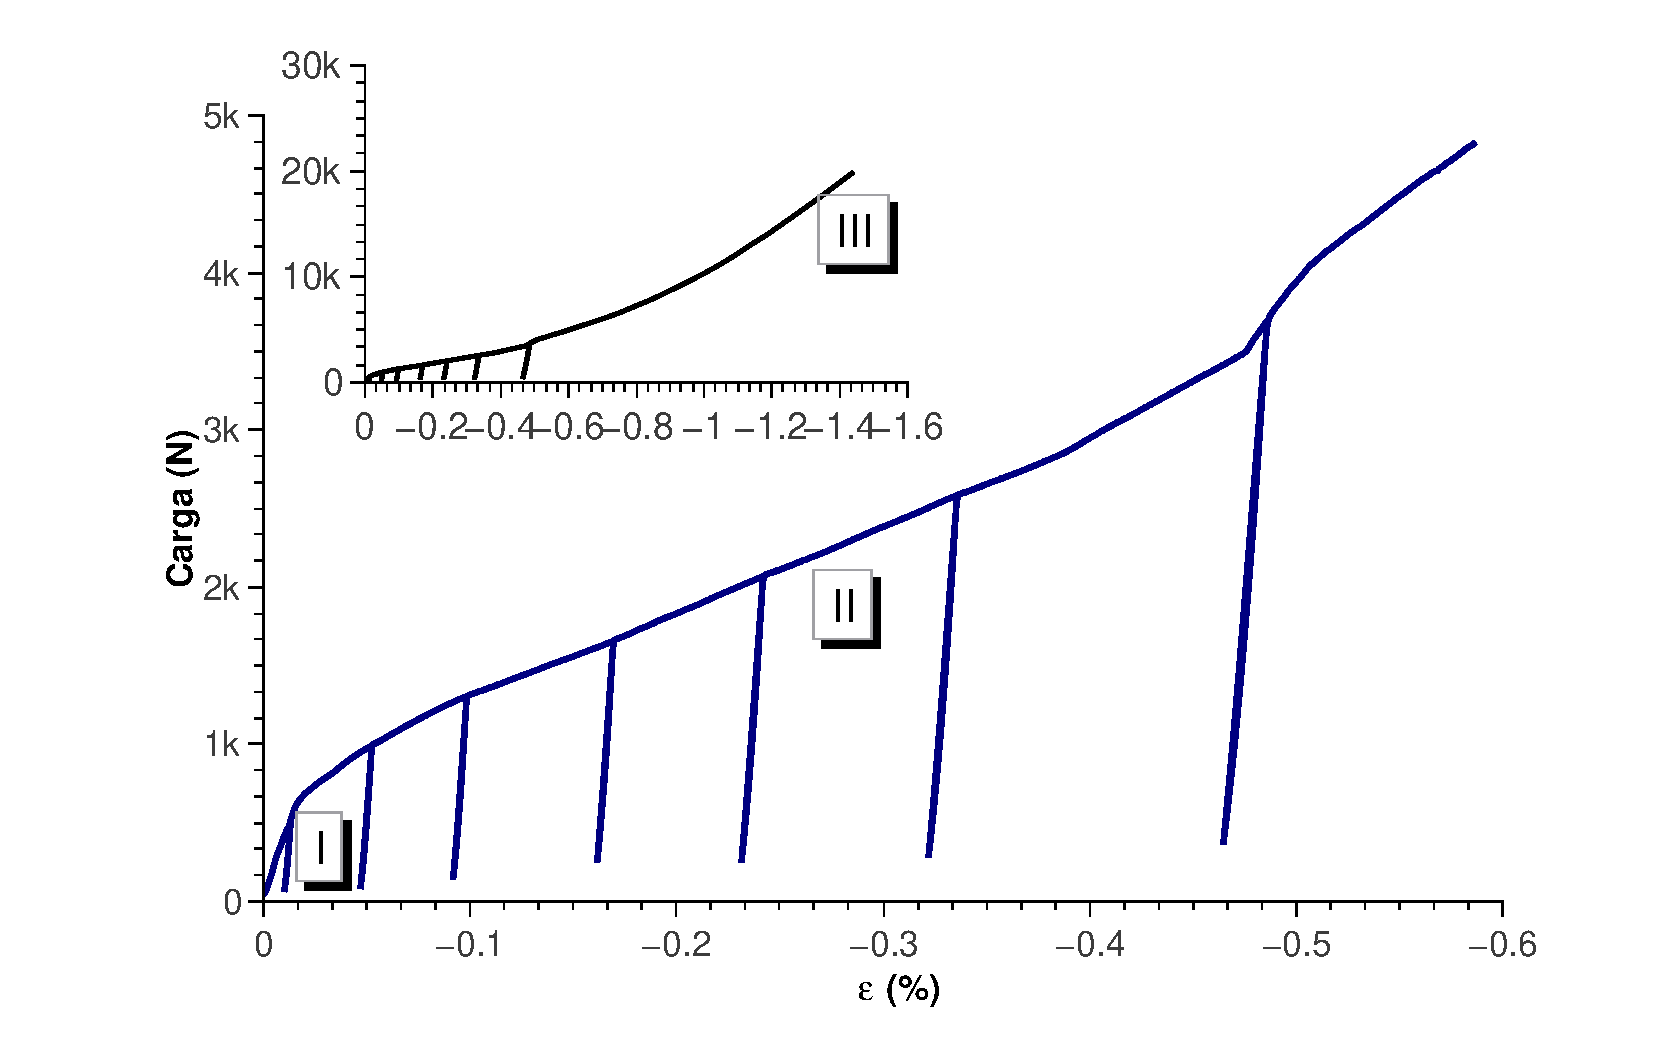
\includegraphics[width=0.9\textwidth]{Img/Introduccion/EspCu.eps}
 \caption{Gráfico de carga vs deformación de una esponja de cobre donde se distinguen las distintas secciones.}
 \label{fig:EspCu} 
\end{figure}

Al aplicar una carga a una esponja y realizar un gráfico tensión vs deformación se distinguen tres tramos, los cuales presentan un comportamiento 
distinto. Como se muestra en la figura \ref{fig:EspCu} Inicialmente se ve un segmento que pareciera ser recto, o sea comportamiento elástico. En el caso de esponjas con celdas abiertas, este tramo 
es más marcado, y la deformación elástica se debe a que las paredes de las celdas se flexionan. En las esponjas con estructuras cerradas el 
comportamiento es más complejo, y la deformación se debe a la flexión de las paredes y el estiramiento de las superficies de los poros. En esta primera 
instancia la pendiente es inferior al modulo de Young de la esponja (E) debido a que ocurre una microdeformación plástica en los puntos más débiles de la 
estructura. Para poder medir la rigidez de la estructura se realiza una carga y luego se mide la pendiente en una descarga.
En el segundo tramo de la curva tensión deformación, puede verse un plateau debido al colapso de la estructura, donde las paredes de las celdas 
comienzan a ceder por fluencia o fracturas. Este palteau se mantiene hasta llegar a una deformación de densificación, donde la estructura ya se encuentra 
comprimida y el módulo elástico aumenta abruptamente. Hay que tener en cuenta que la anisotropía en la forma de las celdas puede llevar a una gran diferencia 
en las propiedades de la esponja en distintas direcciones.

Hay distintas formas con las cuales pueden determinarse las propiedades mecánicas de las estructuras celulares. Una forma muy utilizada es por medio 
de elementos finitos. Otra forma
es a partir de un análisis micromecánico simplificando la estructura como un conjunto de columnas (celdas abiertas), o un conjunto de celdas de catorce caras formadas por cuadriláteros y hexágonos. Si bien esta segunda opción supone una gran simplificación de la estructura se llegan a resultados que concuerdan con los 
resultados obtenidos experimentalmente. Para las estructuras celulares abiertas las principales propiedades mecánicas se describen a partir de la densidad específica \cite{duering} según:

\begin{equation}
\frac{F^*}{F_s}=A \left(\frac{\rho^*}{\rho_s}\right)^n \label{props} 
\end{equation}
Donde $F^*$ es la propiedad de la esponja que se quiere caracterizar, $F_s$ es la característica del material sólido, $\rho^*$ y $\rho_s$ son las 
densidades de la esponja y del sólido respectivamente, $A$ es una constante relacionada a la geometría de la esponja y $n$ otra constante. De acuerdo 
a la ecuación \ref{props} el módulo de Young E \cite{duering} será:
\begin{equation}
\frac{E^*}{E_s}=C_1 \left(\frac{\rho^*}{\rho_s}\right)^2 \label{propsE}  
\end{equation}
%\begin{equation}
% \frac{G^*}{G_s}=C_2 \left(\frac{\rho^*}{\rho_s}\right)^2
%\end{equation}

Donde la constante $C_1$ depende de las características geométricas de la esponja. 
%Por otro lado el módulo de Poisson no depende de la 
%estructura, a partir de mediciones \cite{gibson} se concluyó que su valor está al rededor de $\frac{1}{3}$ para la mayoría de las esponjas. 
Además hay una diferencia entre el módulo E en tensión y compresión, siendo el primero levemente inferior. La ecuación \ref{props} también pude utilizarse 
para describir otras propiedades como la tensión de transformación y la energía disipada/absorbida en ciclos de compresión en el caso de esponjas 
compuestas por materiales con memoria de forma como veremos en la sección \ref{sec:SMF} de este capítulo. 


La tensión a la cual ocurre el colapso de la estructura $(\sigma^*_{pl})$ y la tensión de fluencia del material que la compone $(\sigma_{ys})$  
están relacionadas con la densidad relativa \cite{duering} según:
\begin{equation}
 \frac{\sigma^*_{pl}}{\sigma_{ys}}=C_3 \left(\frac{\rho^*}{\rho_s} \right)^{\frac{3}{2}}
\end{equation}
Donde nuevamente $C_3$ depende de las características geométricas de la estructura. A partir de varias mediciones se llegó a que $C_3 \sim 0.3$ para
la mayoría de las esponjas metálicas \cite{gibson}. 
Es muy importante conocer el valor de $\sigma^*_{pl}$ ya que es la carga a la cual la estructura comienza a colapsar.  Las esponjas metálicas tienen 
un poder de amortiguamiento de entre cinco y diez veces el del material sólido \cite{design} lo que las hace una muy buena opción para aplicaciones 
donde se busca amortiguar cargas. 

La deformación se produce en bandas a $45^\circ$ respecto de la tensión aplicada. Estas bandas suelen tener el espesor de una celda, 
y en ellas la tensión alcanza la tensión de fluencia mientras que en las zonas externas se mantiene en el rango elástico. Debido a esta deformación inhomogenea el material dentro de las bandas se endurece, con lo cual la tensión aplicada no es suficiente para seguir deformándolo, por lo que para poder acomodar la deformación las bandas se ensanchan, deformándose el material contiguo, o bien se generan nuevas bandas.     

% Las bandas donde se 
% concentra la deformación se endurecen, llegan a un punto en que ya no siguen deformándose, por lo tanto o aumentan su espesor o se forman nuevas bandas.

Al comprimir una probeta, las caras exteriores de la misma no sostendrán carga ya que son superficies con menos restricciones.
La carga es soportada por las partes en el interior de la estructura. Gibson \cite{gibson} realizó ensayos variando el tamaño de la muestra 
y concluyó que cuando la esponja tiene 
dimensiones infinitas (mucho mayores a las dimensiones de las celdas) el módulo de Young tiende al valor del módulo de la esponja. A medida que 
las dimensiones disminuyen y se acercan al tamaño de algunas celdas comienzan a actuar los efectos 
de borde, las superficies de la celda comienzan a actuar como concentradores de tensiones y el módulo de Young de la esponja disminuye respecto al del 
material sólido. Es por esto que todas las muestras de esponjas a ensayarse deben tener dimensiones de por lo menos seis a siete celdas, de esta 
forma se asegura que la performance de la esponja no se vea afectada por los efectos de borde.

%\newline %\newline
%\textbf{Modulo de young respecto del tamaño de la esponja respecto del tamaño de la celda}
%\newline %\newline

\begin{figure}[h]
 \centering
 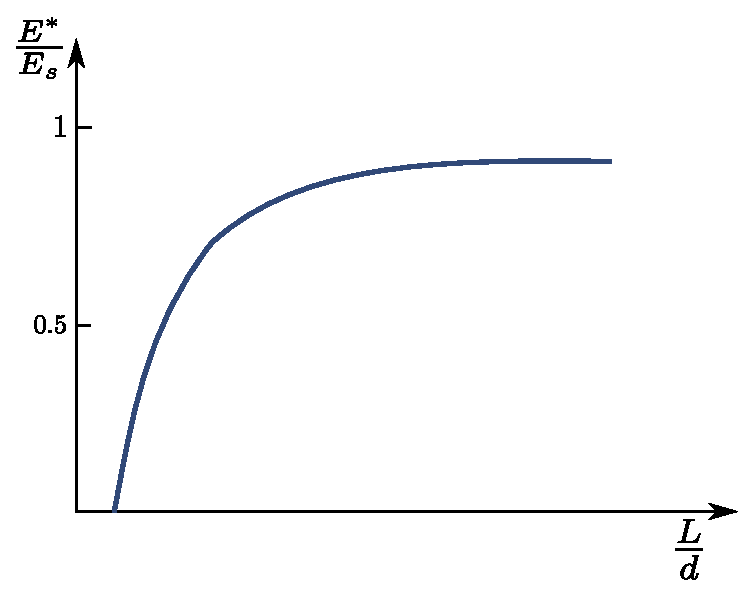
\includegraphics[width=0.5\textwidth]{Etam.eps}
 \caption{Esquema de como varía el Módulo de Young relativo de la esponja. $L$ es el largo de la esponja, $d$ es el tamaño de los poros de 
 la estructura celular, $E^*$ es la rigidez de la esponja y $E_s$ es la rigidez de la esponja con dimensiones infinitas.}
\end{figure}

%Además si las cargas se aplican de forma cíclica la esponja fallará por fatiga. La principal causa son pequeñas fisuras que nuclean y van creciendo a 
%medida que aumenta la cantidad de ciclos a la cual se somete la estructura. También ocurre otro mecanismo llamado creep por ciclado, donde la estructura 
%se va acortando por deformación plástica bajo un esfuerzo cíclico de compresión con un valor medio distinto de cero, y la formación de fisuras frágiles 
%en tensión.

% Fatiga es un fenómeno que ocurre cuando se somete una estructura a una tensión cíclica, la cual oscila entre dos valores determinados. Estos valores 
% pueden ser ambos positivos, ambos negativos o de distintos signos. Se utiliza un parámetro $R$ que relaciona ambas tensiones según:
% \begin{equation}
%  R=\frac{|\sigma_{min} |}{| \sigma_{max} |}
% \end{equation}
% Los ensayos de fatiga consisten en someter a una probeta a cargas cíclicas $(\Delta \sigma = \sigma_{max} - \sigma_{min})$ y evaluar su comportamiento. 
% La probeta puede no sufrir ningún daño, nuclear pequeñas fisuras, o romperse de forma frágil. En un ensayo de fatiga se evalúa para que cantidad de 
% ciclos $(N_f)$ comienzan a nuclearse estas fisuras. 
% %Es un resultado conocido que, a temperatura ambiente, la cantidad de ciclos donde falla la estructura no depende de la frecuencia a la cual se aplican las cargas, sino del valor 
% %máximo de tensiones aplicadas. 
% En ensayos con esfuerzos cíclicos en tensión se define el límite como el número de ciclos a la cual se producen fisuras en la estructura que la llevan a 
% la rotura con un determinado $\Delta\sigma$. En ensayos de compresión el límite se define como el número de ciclos para el cual comienza el colapso 
% de la estructura. 
%  
% Luego se realiza un gráfico $\Delta \sigma$  vs.  $N_f$. Este gráfico aporta información muy importante ya que para las aleaciones metálicas generalmente 
% se llega a una determinada tensión para la cual, utilizando valores inferiores, no ocurrirá la falla del material. Además, por convención, 
% se dice que el material tendrá vida infinita si no falla antes de los $1x10^7$ ciclos. Tanto en compresión como en tracción se obtienen curvas que 
% siguen las siguientes etapas. Una primera etapa donde aumenta la deformación progresivamente, hasta que alcanza una segunda etapa donde se mantiene 
% constante. Finalmente cuando se llega a un número de ciclos $N_T$ la deformación aumenta abruptamente. 
% 
% \begin{figure}[h]
%  \centering
%  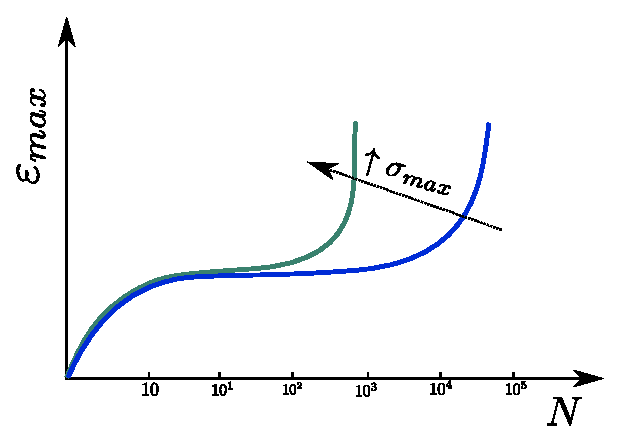
\includegraphics[width=0.6\textwidth]{fatiga.eps}
%  \caption{Esquema de un ensayo de fatiga de una estructura celular donde $N$ es el número de ciclos de deformación. También se muestra como con el aumento de la tensión máxima aplicada disminuye el 
%  número de ciclos para el cual se produce la falla de la estructura.} 
%  \label{fig:fatiga}
%  \end{figure}
% 
% Si se aplica una tensión cíclica con un valor medio positivo, en la etapa dos, las esponjas metálicas sufren un alargamiento debido a un efecto de 
% creep cíclico. Luego se nuclea una fisura en el punto más débil de la estructura, la cual continua creciendo con muy poca deformación plástica. 
% Por otro lado en un ensayo de compresión, luego de un período de incubación, ocurre una mayor cantidad de deformación plástica que en el caso 
% anterior. Se cree que el mecanismo que ocurre es una combinación de fracturas en las paredes de las celdas y en la estructura, sumado a un creep 
% cíclico. Ashby \cite{design} clasifica los distintos tipos de deformación que pueden ocurrir de la siguiente manera:
% \begin{itemize}
%  \item[$\circ$] Fisuras se producen en todo el material, y no se diferencia una banda de deformación acumulada. 
%  \item[$\circ$] La deformación se concentra en distintas bandas. Primero en el punto más débil de la estructura se deforma una banda, una vez que la deformación 
%  alcanza un cierto valor se forma una nueva banda en otro punto débil de la estructura. Los sitios donde se forman las bandas de deformación están relacionados 
%  con la estructura de la misma. 
%  Por ejemplo los sitios de la esponja con mayor densidad pueden mantenerse íntegros, sin deformación plástica.   
%  \item[$\circ$] Se forma una única banda de deformación la cual se engrosa al aumentar los ciclos.
%  \end{itemize}
% 
% Como regla general \cite{design} Al utilizar tensiones más altas, la cantidad de ciclos a la cual se produce la fisura disminuye. Al igual que para los 
% materiales sólidos la vida del material está más relacionado con la tensión máxima aplicada que con la diferencia de tensiones en cada ciclo. 
% 


%\subsection{creep}

%Para usos a alta temperatura es importante conocer el comportamiento de creep a alta temperatura. Se puede ver a partir de entender el pandeo de las paredes de la estructura que 
%forma la estructura abierta. Puede explicarse como :
%\begin{equation}
% \dot{\varepsilon}=\varepsilon \left( \frac{\sigma}{\sigma_0} \right) ^n
%\end{equation}

%$\dot{\varepsilon}$, $\sigma_0$ y n son constantes del material sólido que compone la esponja.

%\...\...\...\...\... sigue calculando los valores de creep para la esponja

%\subsection{fatiga}





\section{Esponjas con memoria de forma }
\label{sec:SMF}

\begin{figure}[h]
 \centering
    \begin{subfigure}{0.49\textwidth}
        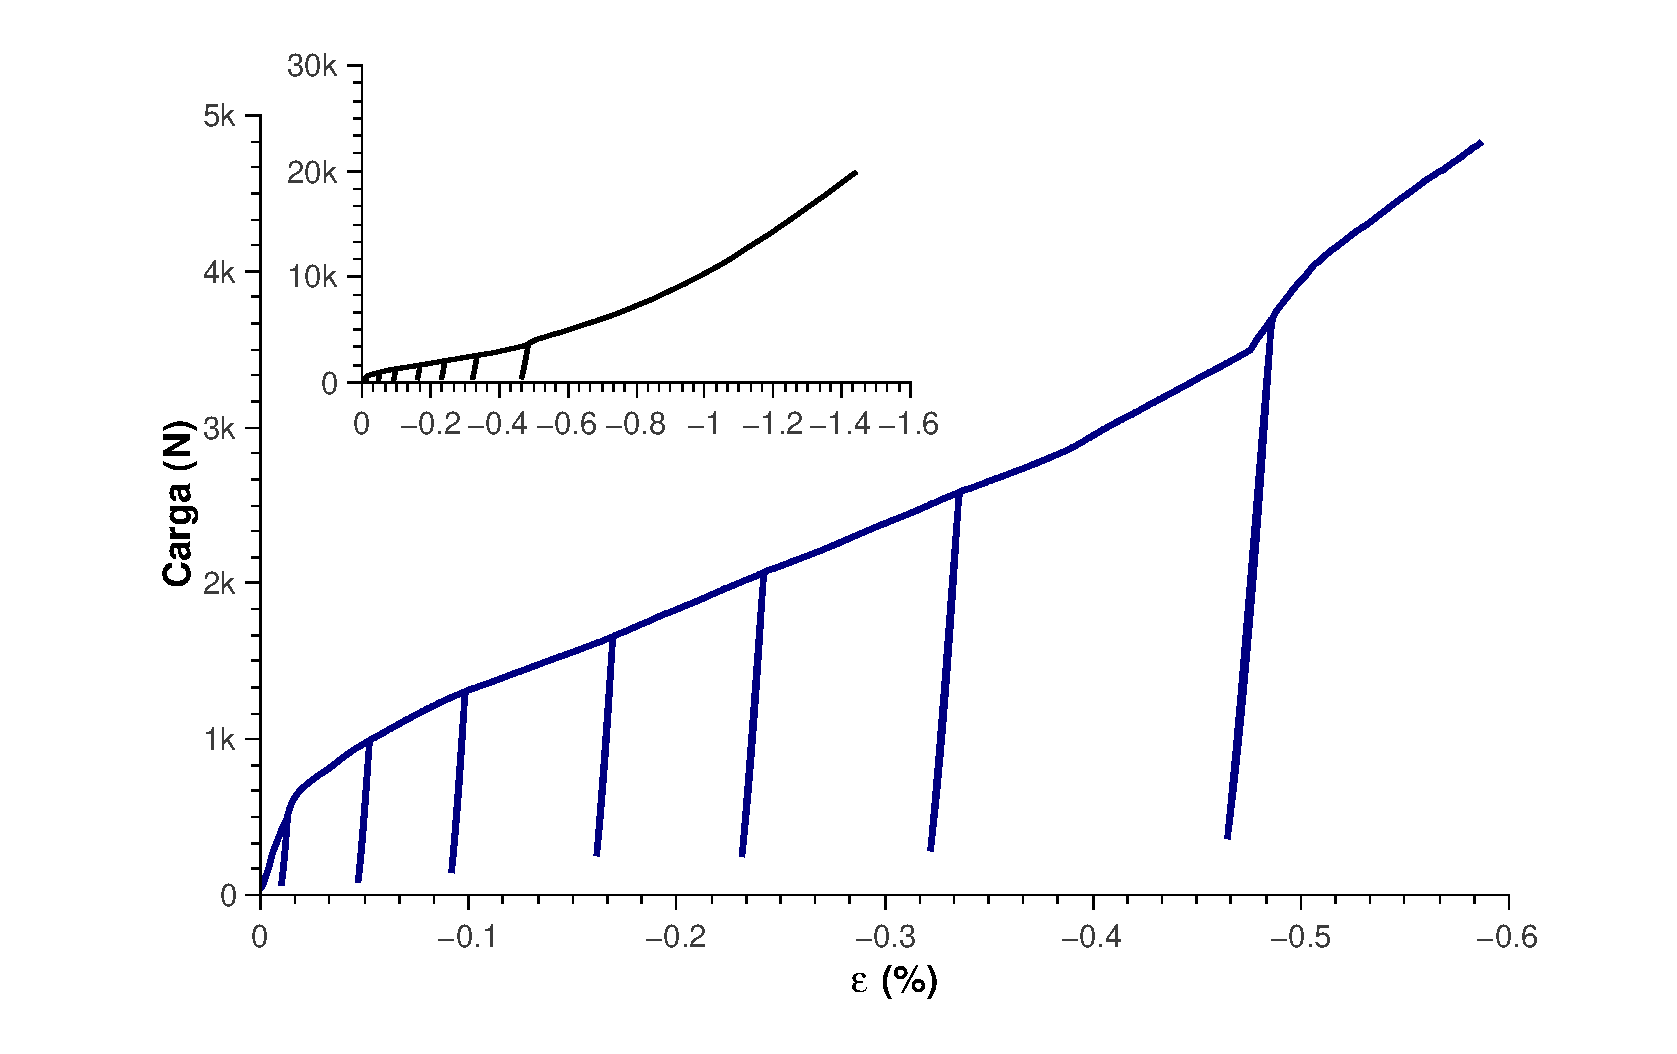
\includegraphics[width=\textwidth]{Img/Introduccion/Cucompararesponja.eps}
        \caption{EspCu2}
        \label{fig:}
    \end{subfigure}
    \begin{subfigure}{0.45\textwidth}
        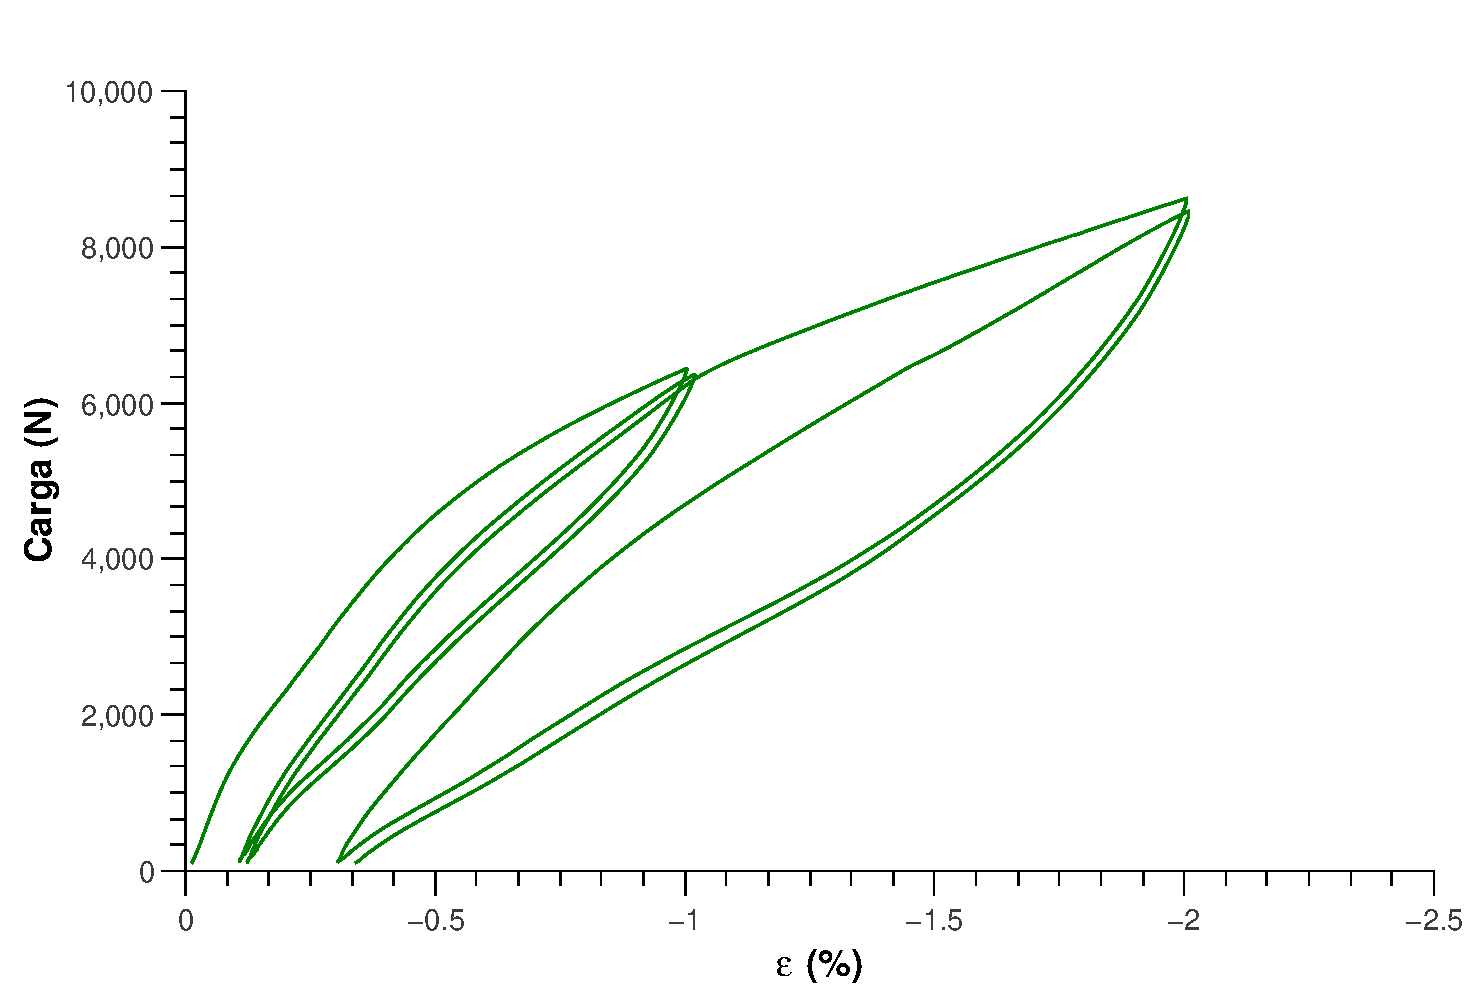
\includegraphics[width=\textwidth]{Img/Introduccion/EsponjacompararCu.eps}
        \caption{}
        \label{fig:EspA}
    \end{subfigure}

  \label{fig: proceso}
  \caption{Comparación de dos diagramas carga vs deformación de \textbf{(a)} una esponja de Cu y \textbf{(b)} una esponja con memoria de forma de Cu-Zn-Al.}
\end{figure}
%\textbf{Gráficos deformación esponja de Cu y Esponja Cu Zn Al}


Como dijimos las esponjas metálicas tienen una capacidad de absorción mucho mayor a la del mismo metal sólido. Si a esto se le suma la absorción en energía 
debido a la pseudoelasticidad generada por la transformación martensítica, tenemos una estructura con gran capacidad de amortiguamiento y muy bajo 
peso. En otras palabras, la energía que se utilizaba en una esponja no pseudoelástica para deformar plásticamente, se utiliza ahora para la transformación
martensítica. Como esta transformación es reversible una vez que se relaja la tensión aplicada la estructura vuelve a austenita recuperando su forma 
inicial. En una curva compresión-deformación (figura \ref{fig:EspA}) se identifican distintas regiones correspondientes a cada uno de estos comportamientos. Inicialmente un 
segmento lineal correspondiente a la deformación elástica de la estructura. Luego hay un cambio en la pendiente, donde comienza a ocurrir 
la transformación martensítica por la tensión aplicada. En este segmento el comportamiento también es prácticamente lineal. Si ahora se libera la carga 
aplicada, la estructura volverá a su forma original. Puede verse que la curva de deformación en un sentido y otro no “siguen un mismo camino”, esto es, 
la curva presenta una histéresis (comportamiento pseudoelástico). En la figura \ref{fig:FisurasEsponja} se muestran micrografías de una esponja donde se distinguen los granos y las placas de martensita formadas al aplicar una carga en la esponja.


 \begin{figure}[h]
 \centering
    \begin{subfigure}{0.45\textwidth}
        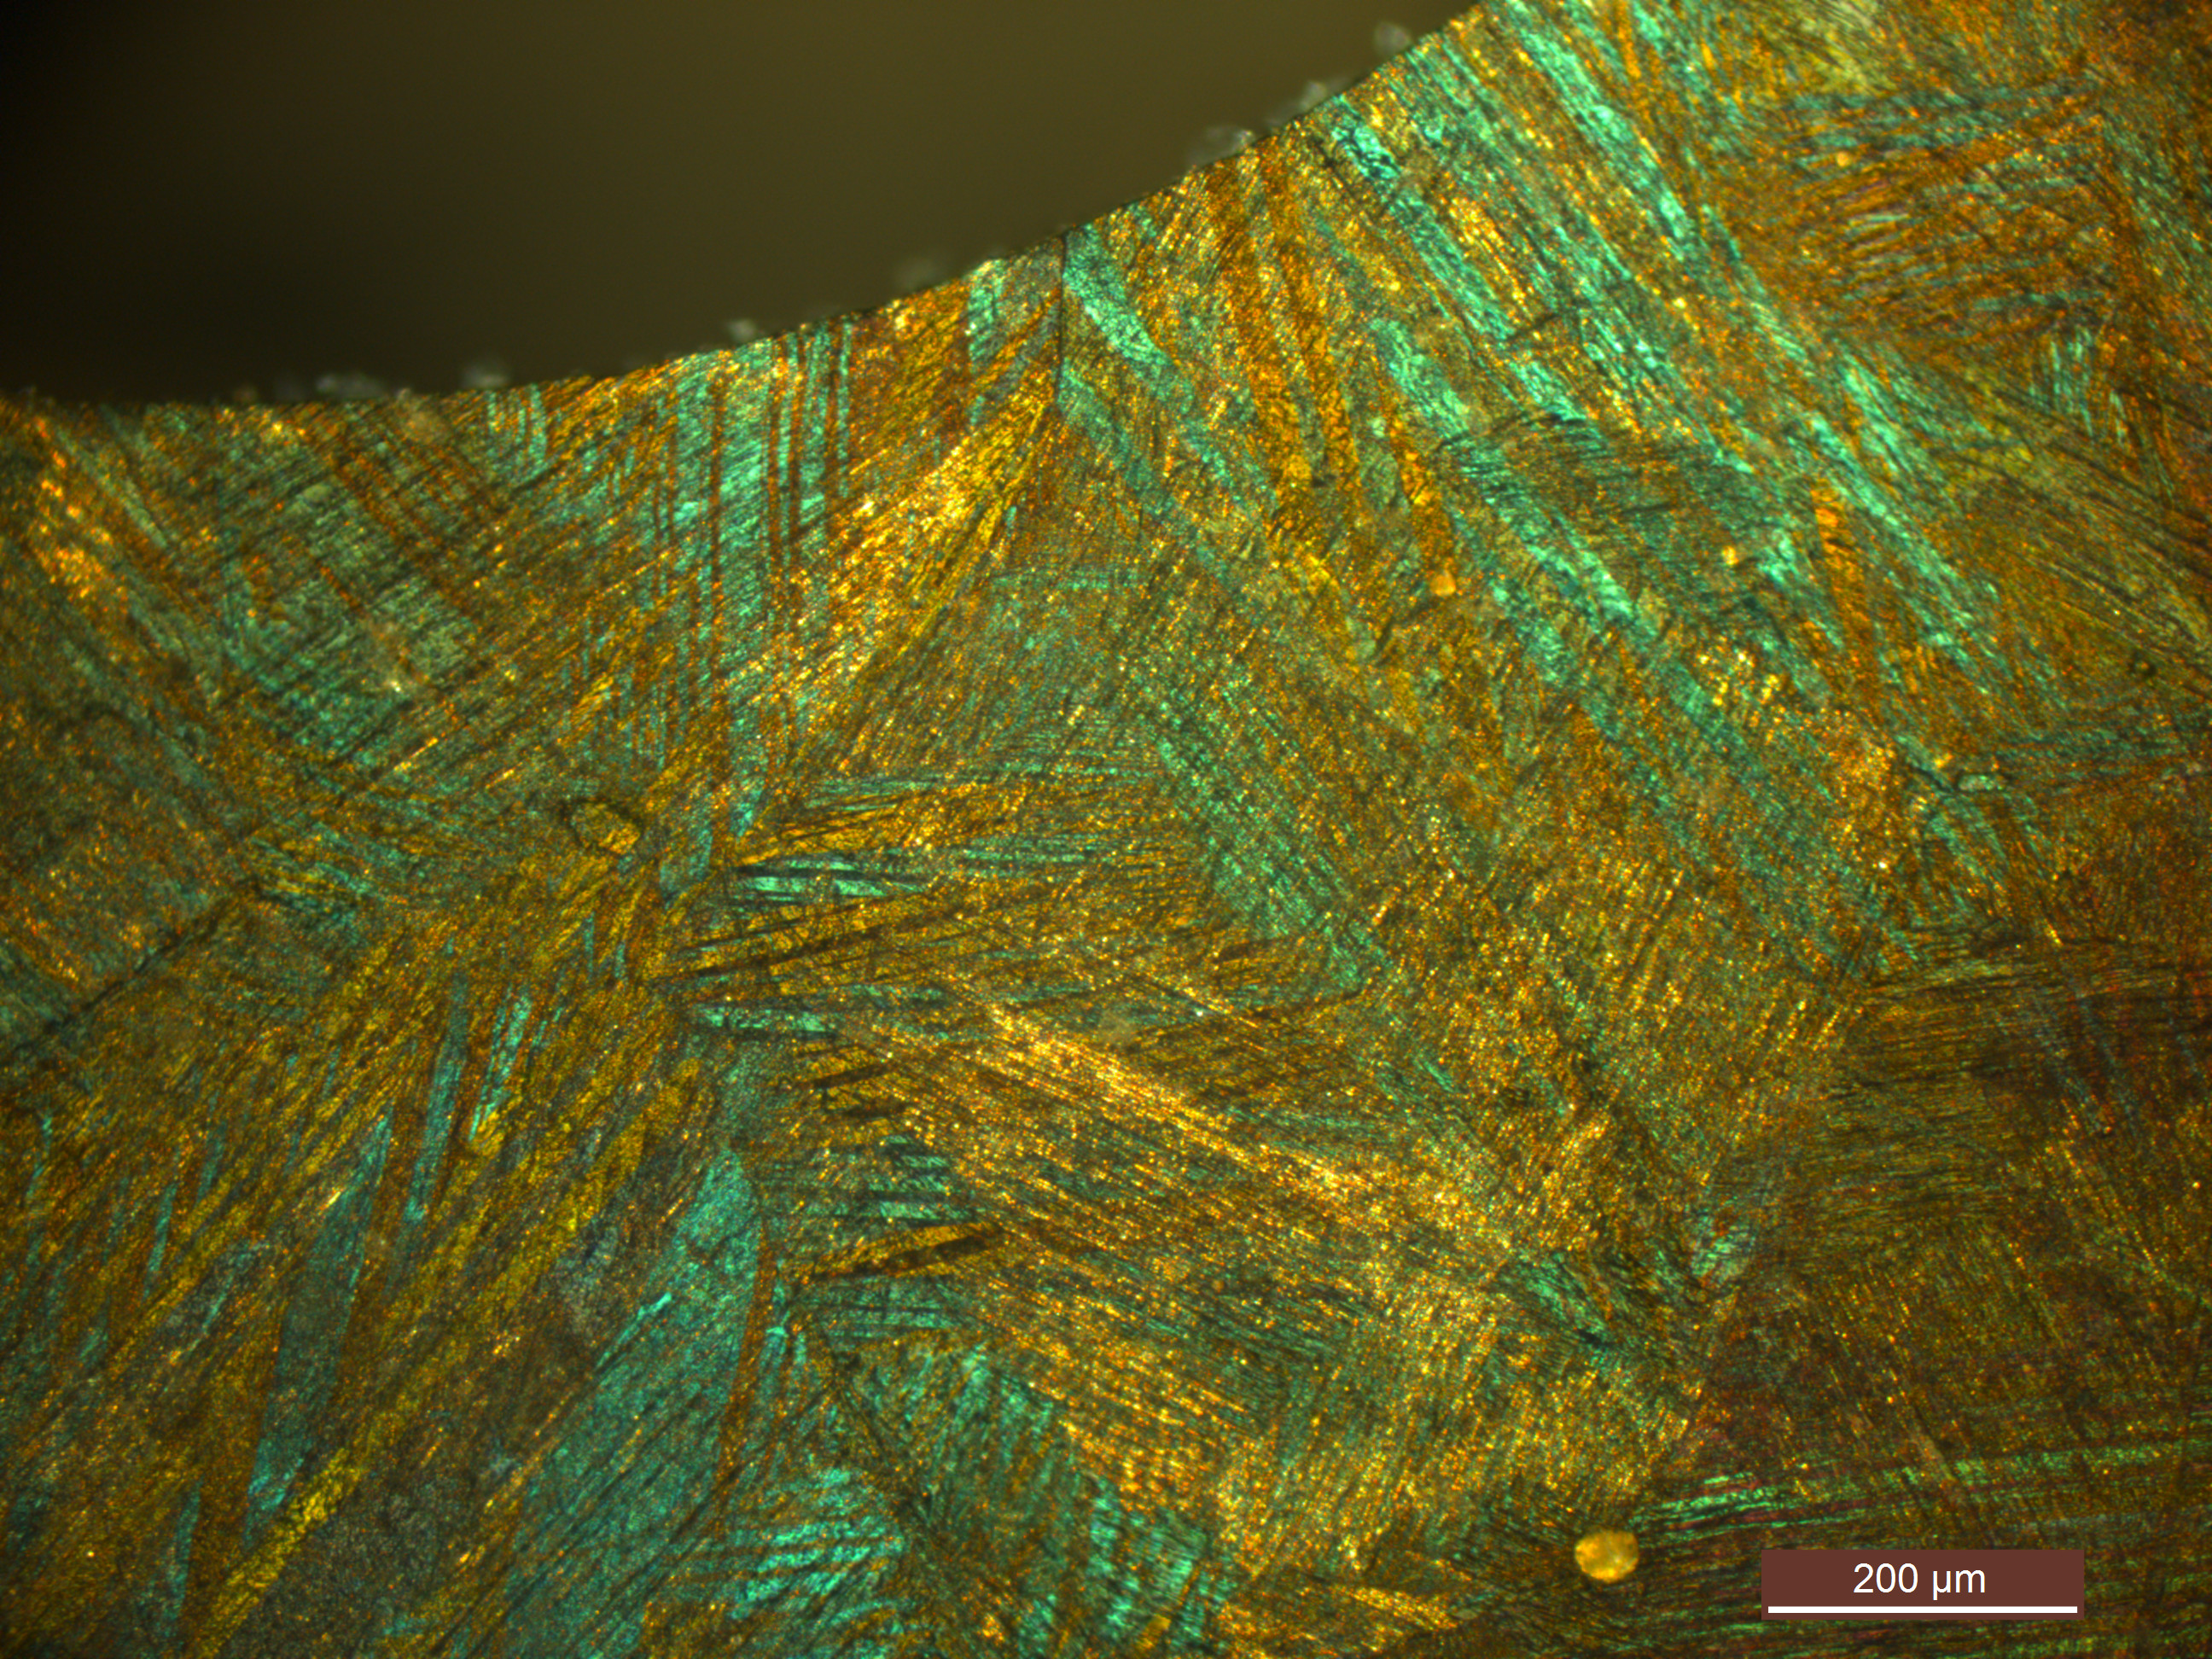
\includegraphics[width=\textwidth]{Img/Introduccion/EspAMicro5.jpg}
        \caption{}
        \label{fig:EspAMicro5}
    \end{subfigure}
 \begin{subfigure}{0.45\textwidth}
        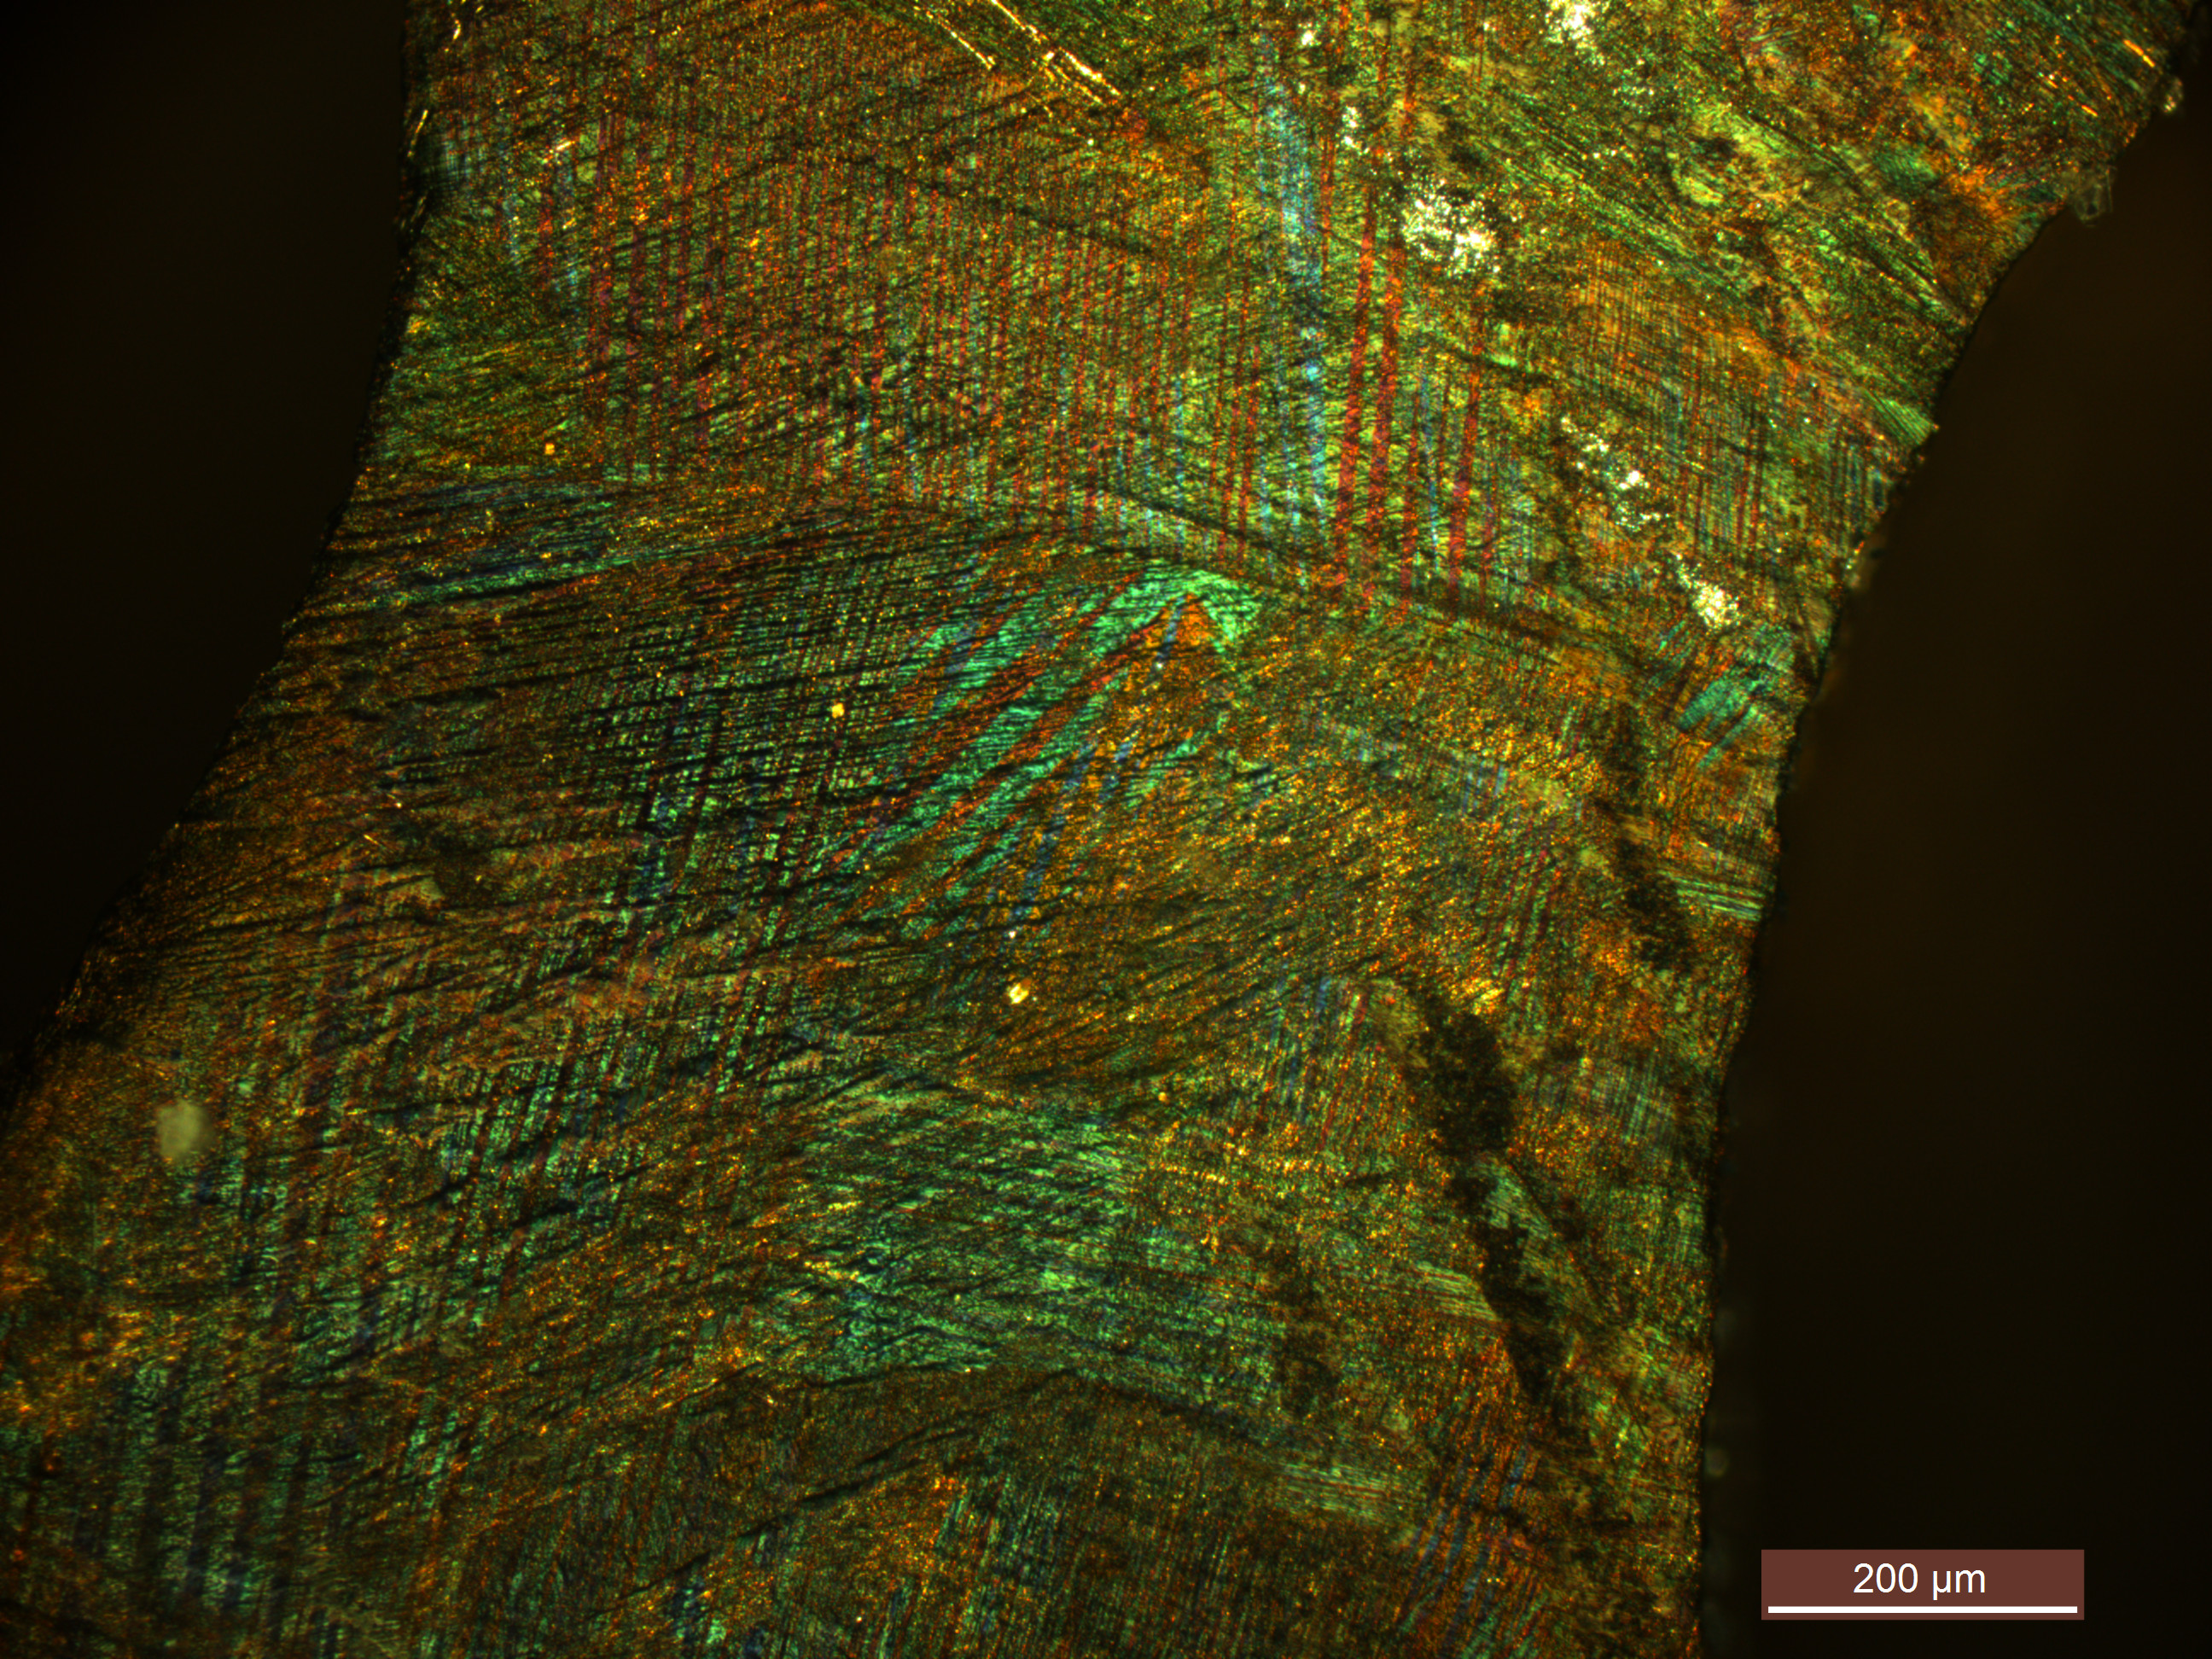
\includegraphics[width=\textwidth]{Img/Introduccion/EspAMicro1.jpg}
        \caption{}
        \label{fig:EspAMicro1}
    \end{subfigure}
    \begin{subfigure}{0.45\textwidth}
        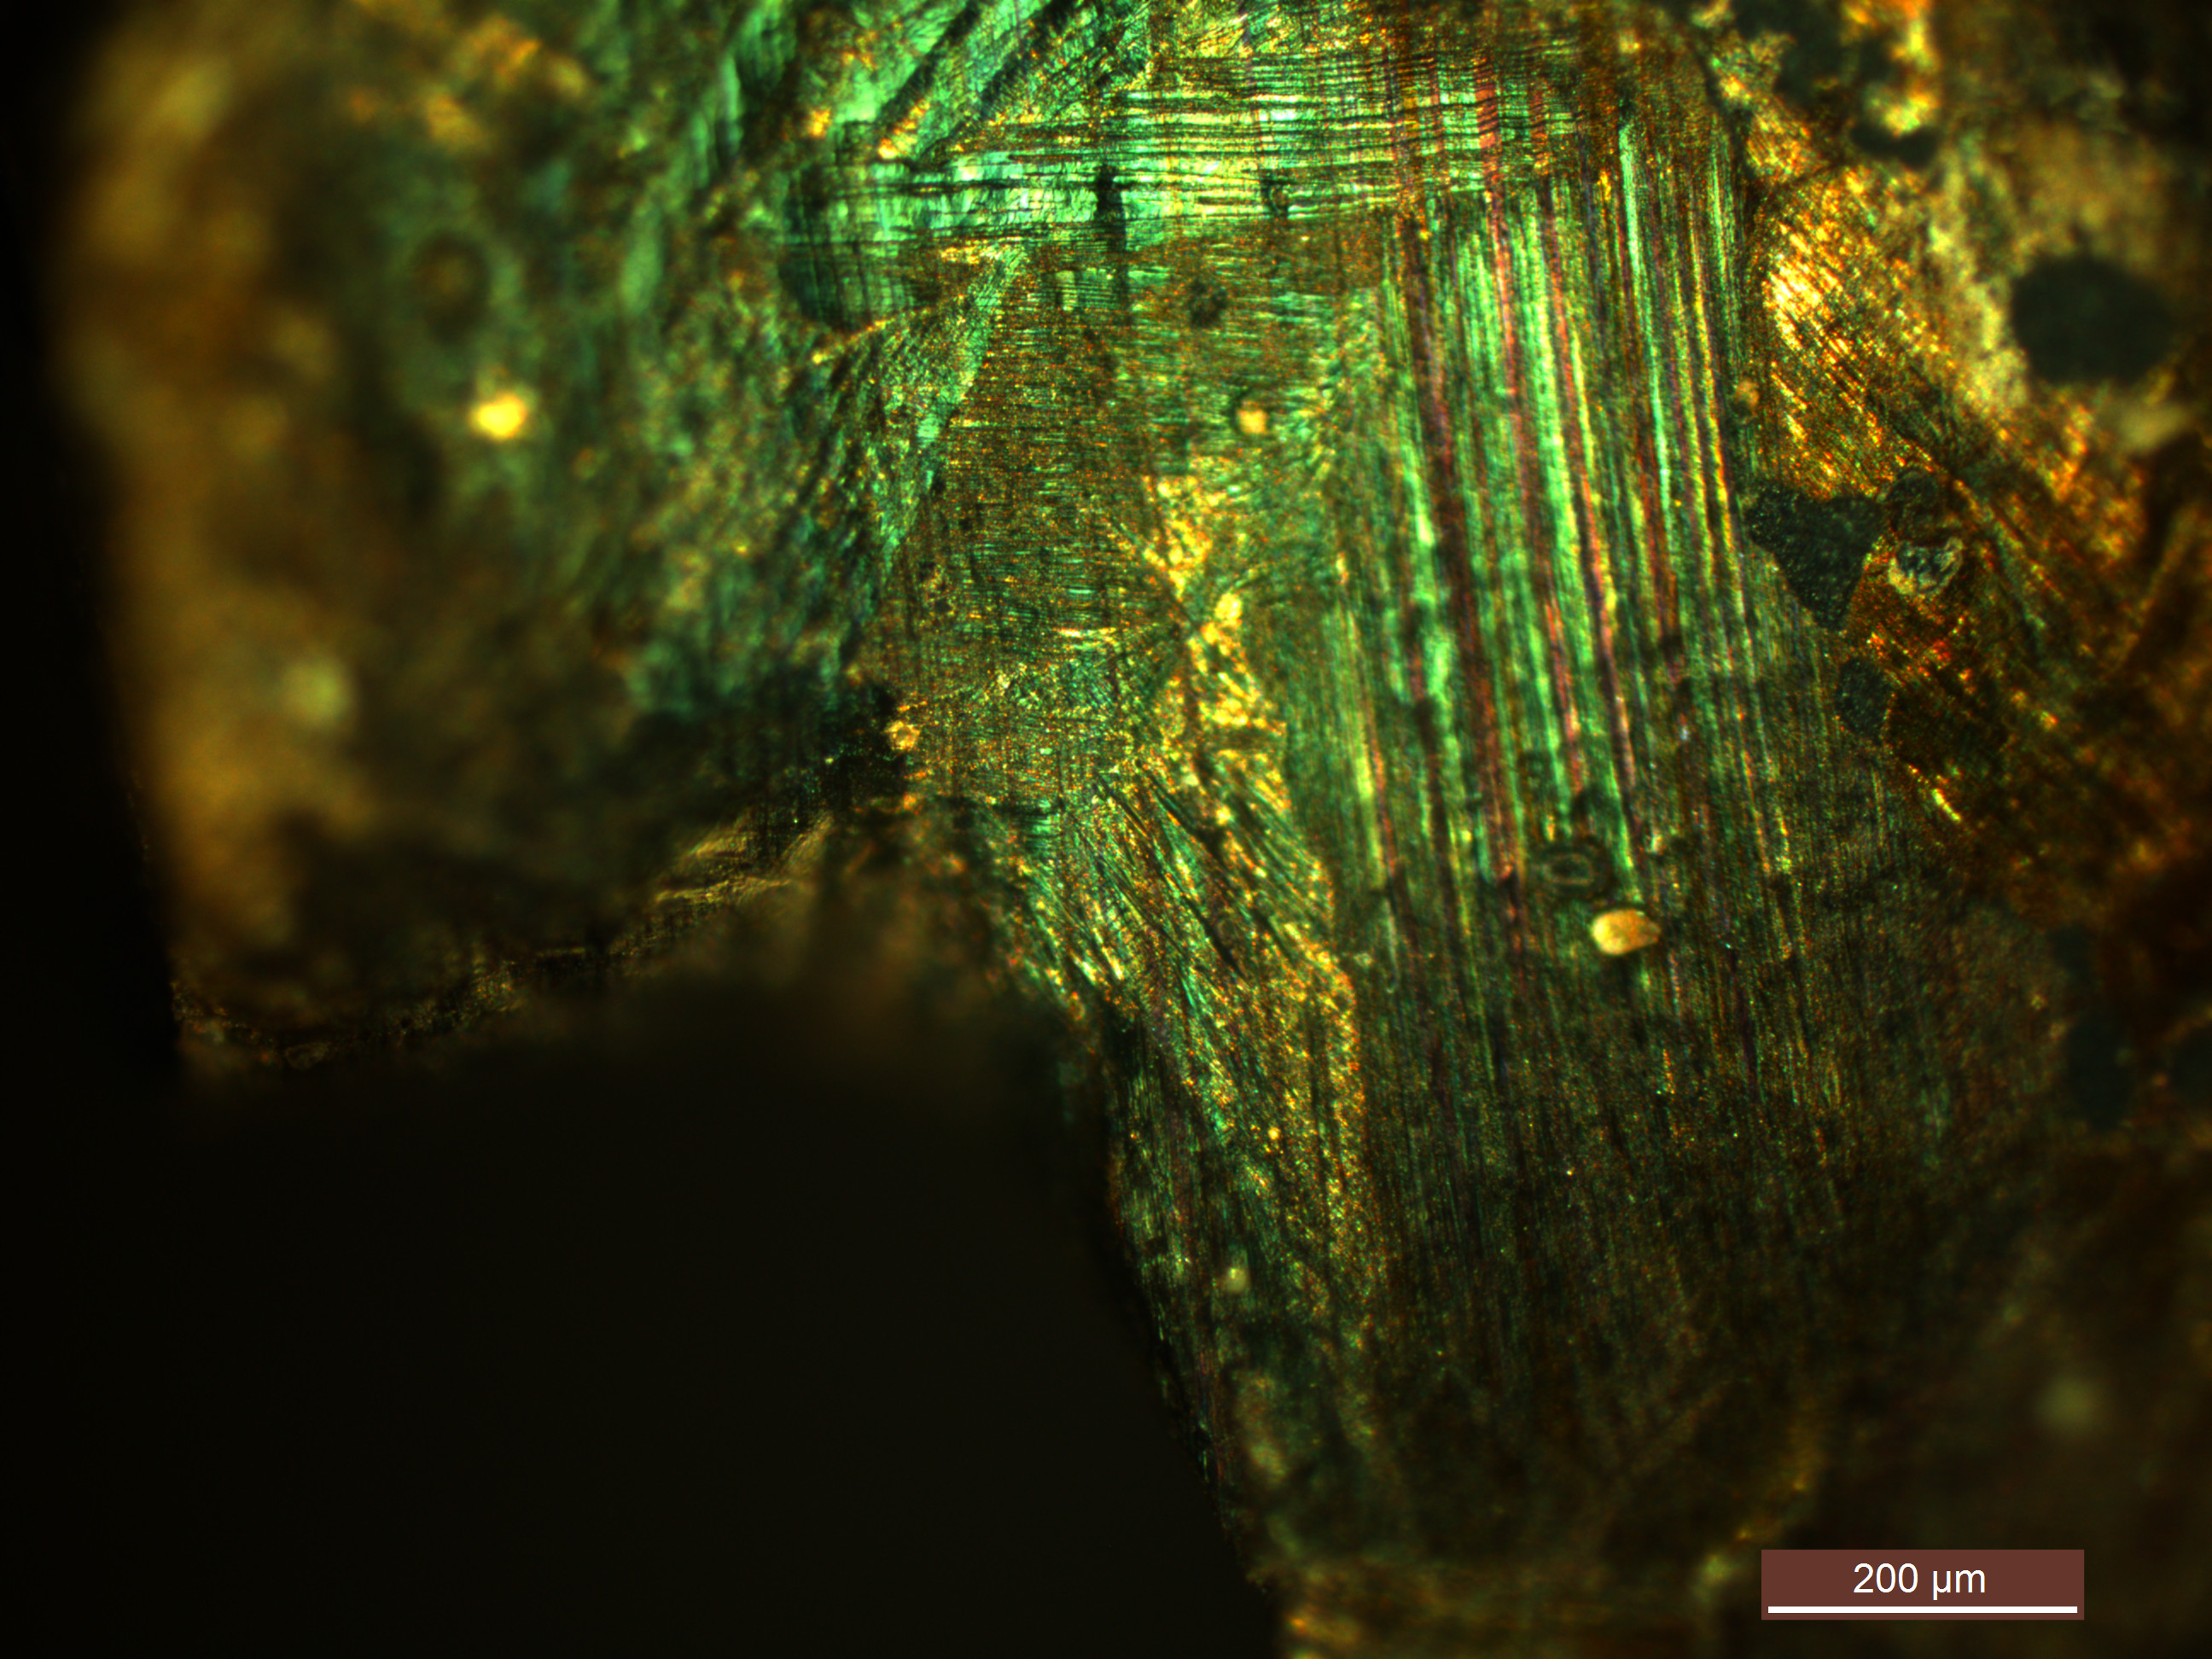
\includegraphics[width=\textwidth]{Img/Introduccion/EspAMicro2.jpg}
        \caption{}
        \label{fig:EspAMicro2}
    \end{subfigure}
     \begin{subfigure}{0.45\textwidth}
        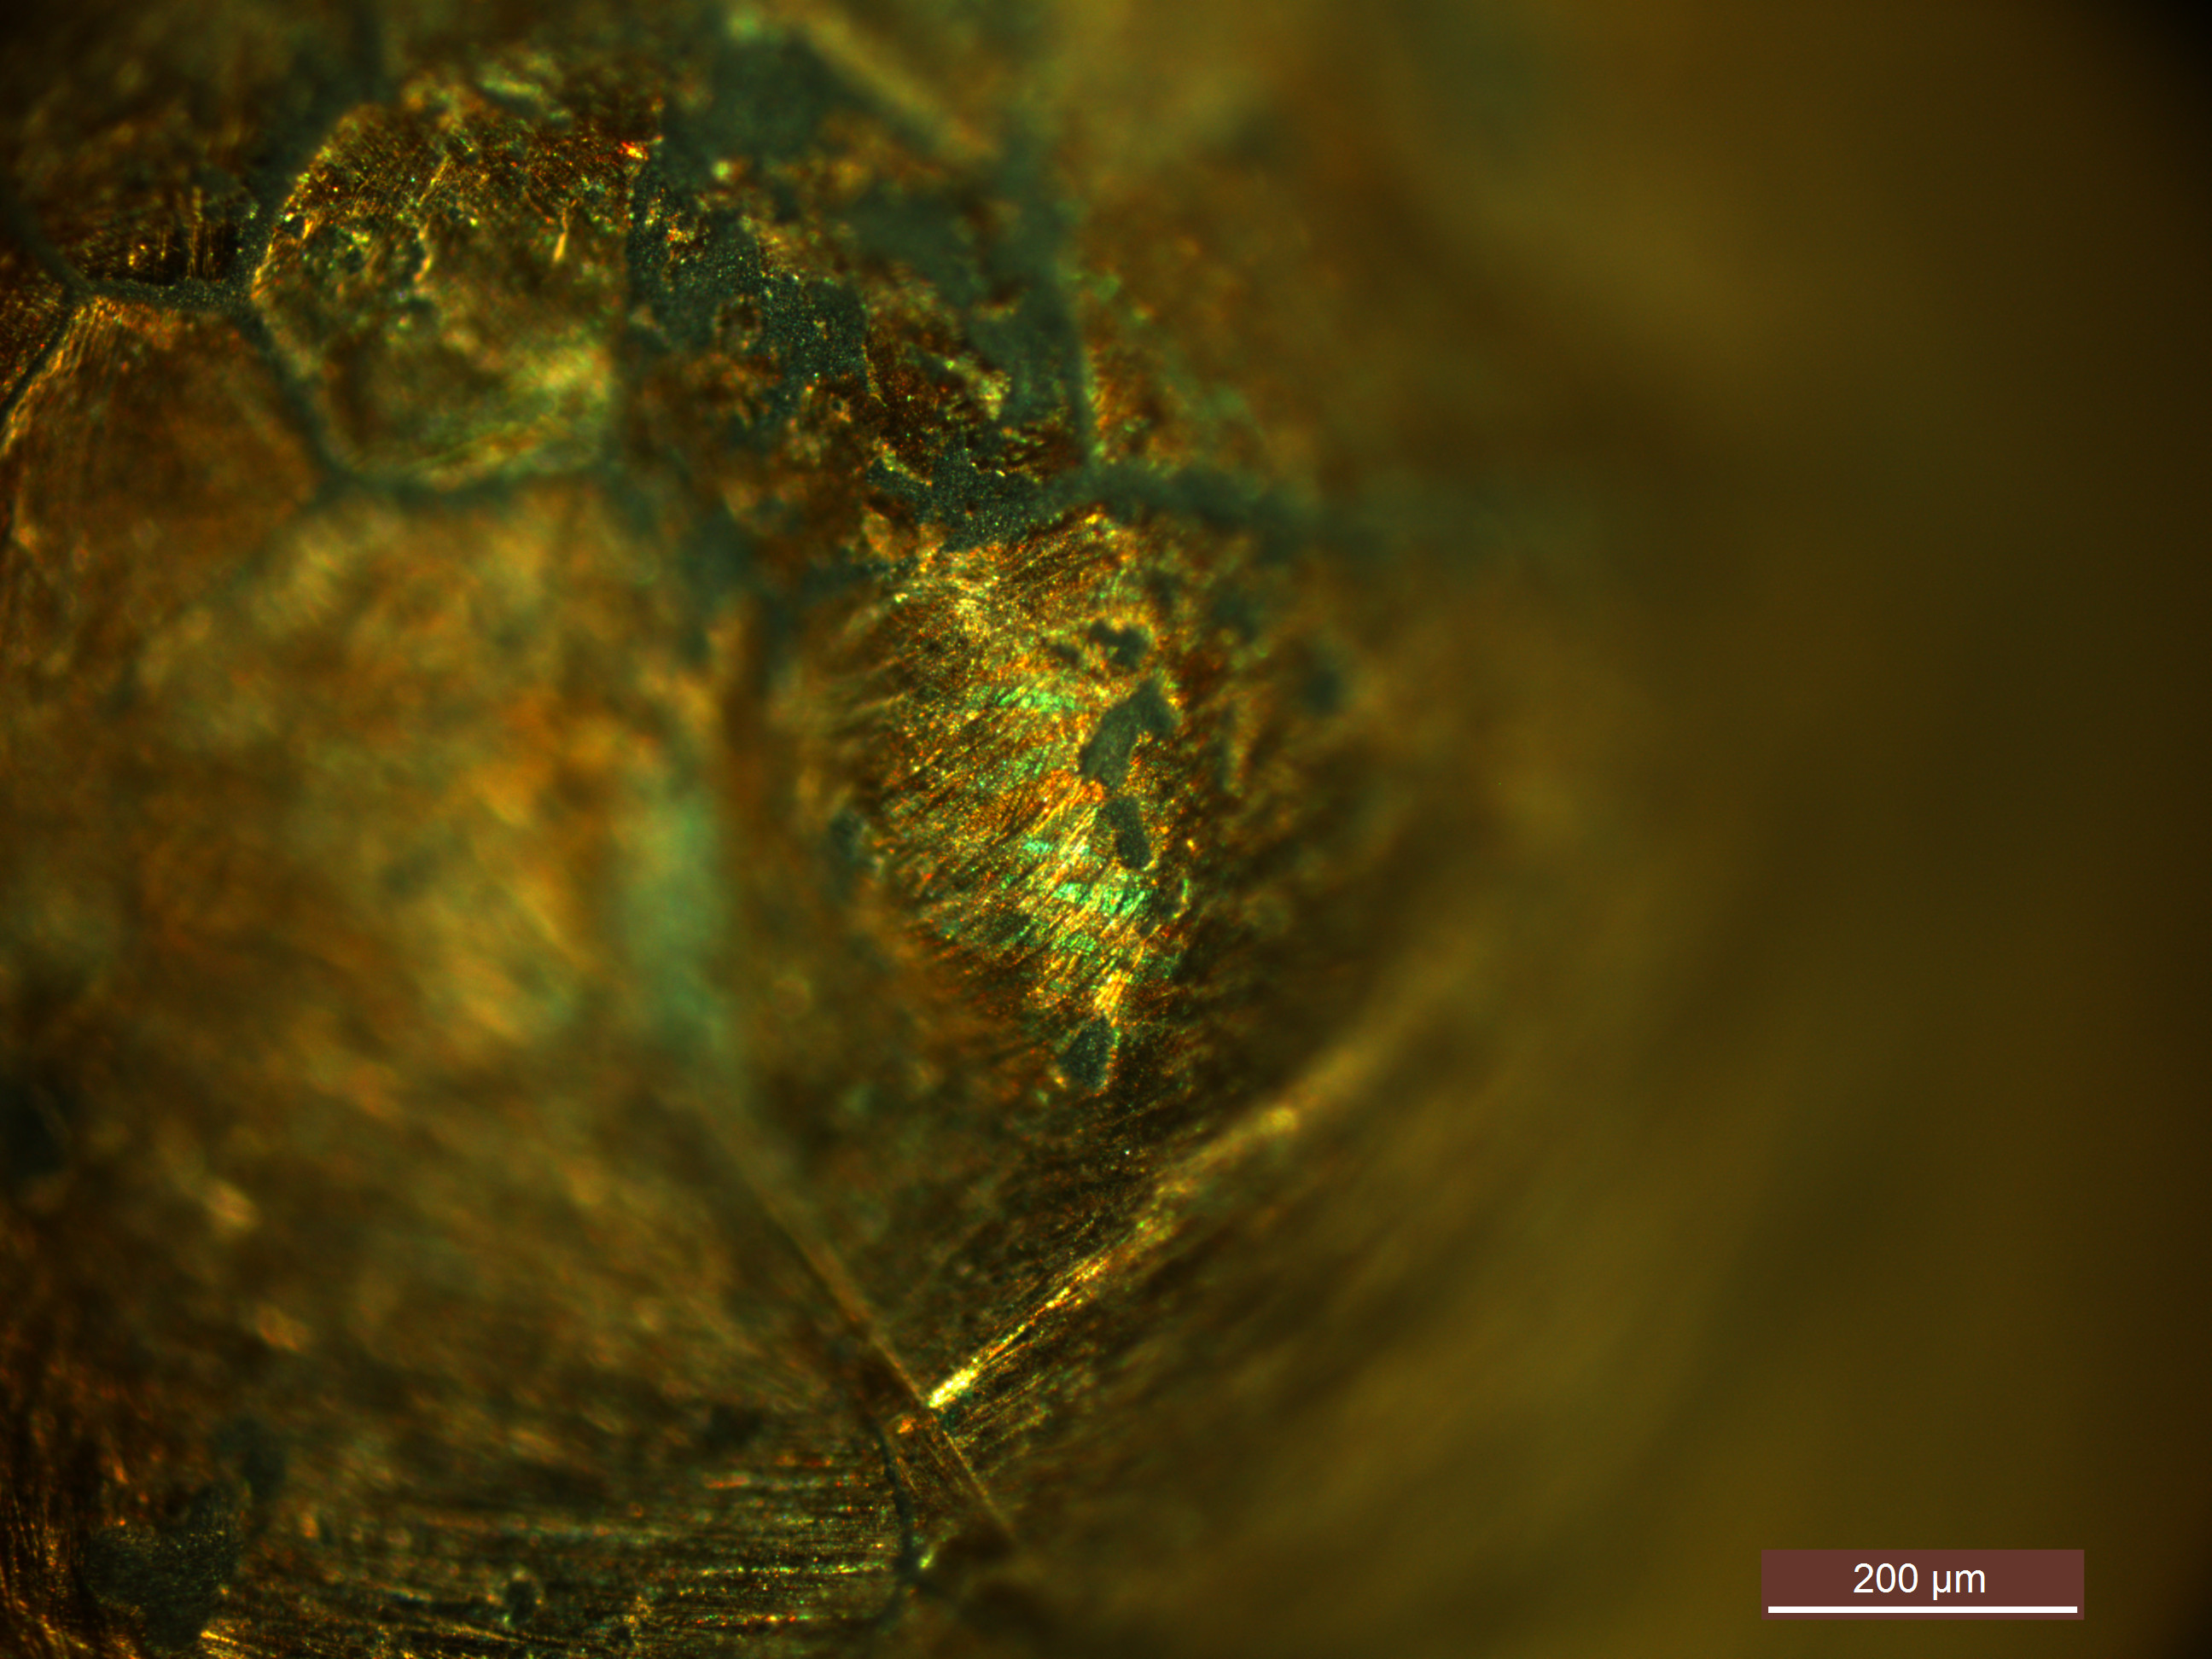
\includegraphics[width=\textwidth]{Img/Introduccion/EspAMicro3.jpg}
        \caption{}
        \label{fig:EspAMicro3}
    \end{subfigure}
 \caption{Micrografías obtenida por microscopía óptica de una esponja. En (a) y (b) se muestran placas de martensita en la cara superior de la esponja. En (c) y (d) se distinguen los granos con algunas placas de martensita en un poro de la esponja.}
  \label{fig:MicrografiasEsponja}
  \end{figure}

Al realizar un esfuerzo en un material macizo la tensión a la cual cambia la pendiente de la curva tensión deformación se llama tensión crítica. Esta 
tensión está relacionada con la tensión necesaria para la formación de martensita. Como vimos anteriormente esta tensión aumenta linealmente con la temperatura según la 
ecuación de Clausius Clapeyron. Cuando se alcanza un determinado valor de temperatura, la tensión crítica comienza a disminuir. Este descenso corresponde a que ahora la tensión crítica 
coincide con la tensión de fluencia del material. Esto puede corroborarse extrapolando la pendiente de este segmento hasta temperatura ambiente, y se encuentra que a esta 
temperatura la tensión crítica coincide con la tensión de fluencia del material. En este punto como la tensión crítica para formar martensita es mucho menor, el 
material formará martensita antes de deformarse. A temperaturas mucho más altas, el material se deformará y no transformará a martensita.

 \begin{figure}[h]
 \centering
    \begin{subfigure}{0.45\textwidth}
        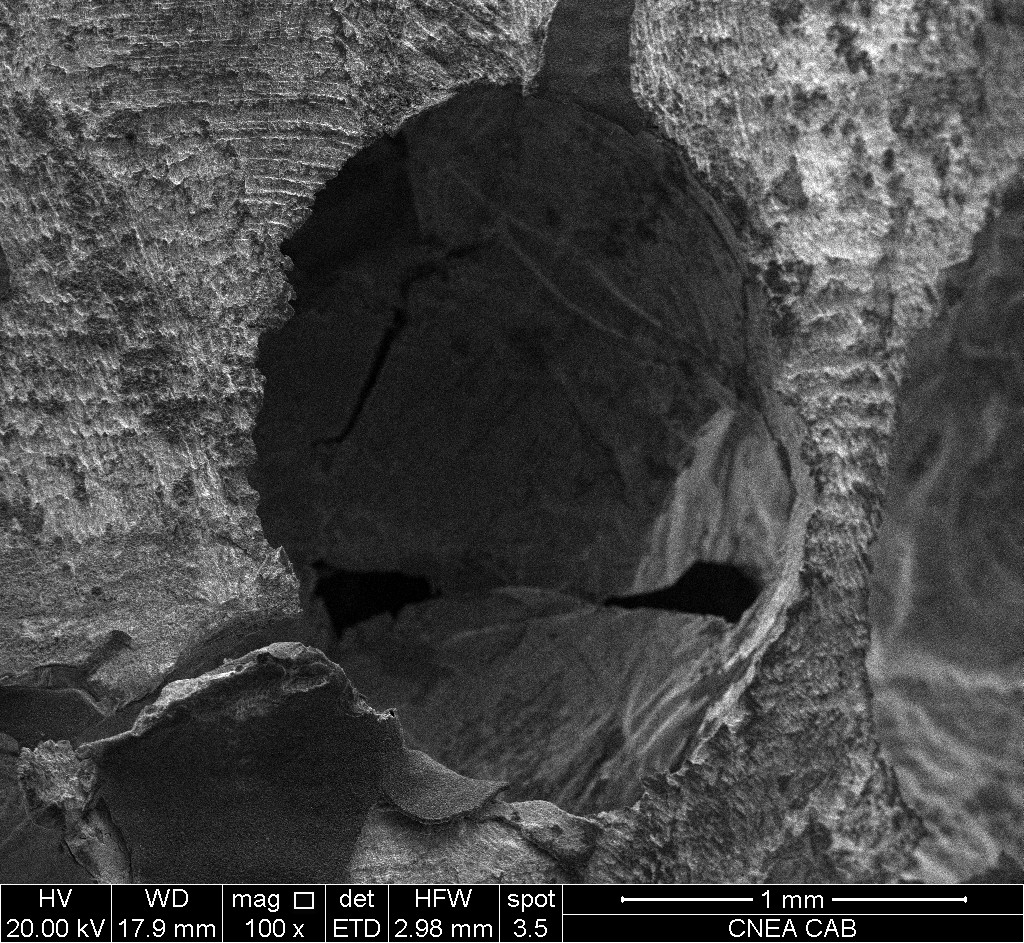
\includegraphics[width=\textwidth]{Img/Introduccion/EsponjaA_004.jpg}
        \caption{}
        \label{fig:}
    \end{subfigure}
    \begin{subfigure}{0.45\textwidth}
        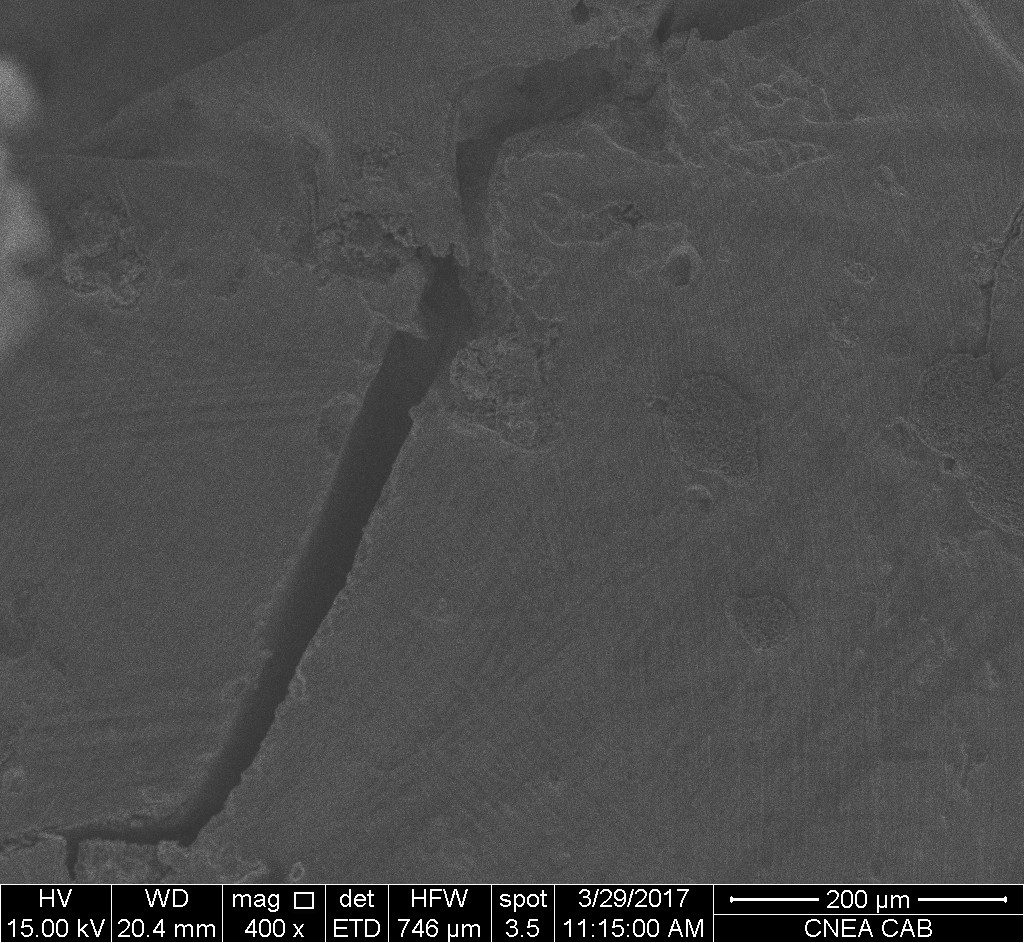
\includegraphics[width=\textwidth]{Img/Introduccion/EsponjaA_005.jpg}
        \caption{}
        \label{fig:EspAa}
    \end{subfigure}
  \caption{Micrografías obtenidas por microscopía SEM de una fisura intergranular en el fondo de un hueco de una esponja.}
  \label{fig:FisuraEsponja}
  \end{figure}

Cuando describimos el comportamiento de los materiales con memoria de forma vimos que en la curva tensión deformación hay un plateau durante el cual la tensión se 
mantiene constante a medida que avanza la transformación martensítica. Al ver el gráfico de deformación de una esponja con material pseudo elástico no aparece este plateau, 
sino que ocurre un cambio en la pendiente (a partir de la tensión crítica). Esto se debe a que el plateau aparece en el caso de deformarse una probeta monocristalina. 
La esponja está compuesta por distintos granos, cada uno con una orientación distinta, por lo que la tensión resuelta en cada uno es distinta. Así cada grano transformará 
a distintos niveles de tensión aplicada. En la figura \ref{fig:MicrografiasEsponja} se muestran micrografías donde se distinguen los granos y placas de martensita en la cara superior de la esponja y dentro un poro. Además la deformación comienza en puntos cercanos a los poros, ya que actúan como concentradores de tensiones. Resumiendo, 
aumentando la tensión aplicada se logran transformaciones en los granos con orientaciones menos favorables para transformar, y además la deformación llega a regiones ubicadas más lejos 
de los concentradores de tensiones.

La transformación de granos con direcciones preferenciales también colabora en la fractura del material de forma intergranular. Esto ocurre ya que los granos que no se encuentran
en direcciones favorables no se pueden acomodar al movimiento de los granos que sí transforman. En la figura \ref{fig:FisuraEsponja} se muestra una micrografía tomada por microscopía SEM de una fisura intergranular. Aunque estas fallas generan una disminución en la performance de las esponjas,
no es significativa ya que estas fisuras pueden tomarse como nuevos poros de la estructura \cite{bertolino2010}. Claramente este comportamiento se da mientras el tamaño de las fisuras no es muy 
grande.

Las propiedades de las esponjas con memoria de forma, como el módulo de Young E, tensión de transformación y la energía absorbida/disipada en un ciclo de 
transformación también pueden describirse según la ecuación \ref{props}. Por ejemplo Gibson \cite{gibson} calcula para esponjas metálicas, utilizando la 
ecuación \ref{propsE}, A=0.98 y n=2. Mientras que Bertolino \cite{bertolino2011} llega experimentalmente a que esta ecuación es aplicable a esponjas 
con memoria de forma, encontrando por ejemplo que para la ecuación \ref{propsE} $A=1$ y $n=2.31$, valores muy cercanos a los anteriores.



% ****************************************************************************************************************************************************
% **************************************************************************************************************************************************** 
% ****************************************************************************************************************************************************

\chapter{Procedimiento Experimental}



\section{Preparación de la aleación} \label{preparacion_aleacion}


Como material de partida para la aleación se utilizaron metales de pureza comercial y se fabricaron lingotes de 80 g con una composición electrónica de 
$e/a=1.48$. Como se mostró anteriormente las propiedades de la aleación pueden variar ampliamente 
con pequeños cambios en la composición, por lo que cada uno de los metales se pesaron con balanza de precisión (con una mínima resolución de $0,001g$). 
Luego se les realizó un pulido químico con las siguientes soluciones:
\begin{itemize}
 \item[$\circ$] Cu: $50 \%$ ácido nítrico (al $65 \%$) - $50 \%$ agua
 \item[$\circ$] Zn: $60 \%$ ácido nítrico (al $65 \%$) - $40 \%$ agua
 \item[$\circ$] Al: $60 \%$ agua - $30 \%$ ácido clorhídrico (al 37 \%) - $10 \%$ ácido fluorhídrico (al $48 \%$)
\end{itemize}

Una vez pesados y pulidos cada uno de los metales, se colocaron en una ampolla de cuarzo con una atmósfera de argón. Luego se colocó la ampolla en 
un horno resistivo a aproximadamente $1100^\circ C$, temperatura superior a la temperatura de fusión de cada uno de los metales. Por último se abrió la ampolla, y se extrajo un 
lingote de la aleación buscada la cual se pesó para cuantificar la cantidad de material que se perdió en el proceso.  

Antes de ser utilizada, la aleación ya fabricada se sumergió en una solución de $50 \%$ ácido nítrico (al $65 \%$) y 
$50 \%$ agua para quitar óxidos e impurezas que hayan quedado del proceso de fundición hasta que se observó una superficie más limpia y brillante.

\section{Reducción del tamaño de grano} \label{FabClavos}


Las propiedades mecánicas dependen en gran medida del tamaño de grano del material. Tanto en el material sólido como en las esponjas, para que las agujas de martensita no tengan tantos obstáculos que impidan su crecimiento, se busca un tamaño de grano relativamente grande. Por otro 
lado, al someter la estructura a esfuerzos de compresión, si el grano es muy grande se producen fisuras intergranulares. Esto genera 
una disminución en las propiedades mecánicas. El principal método para evitar las fracturas intergranulares debido a la anisotropía elástica es el refinamiento de la estructura por medio de trabajado mecánico. Como la estructura 
celular de las esponjas se obtiene en la solidificación del metal fundido, resulta evidente que no es posible utilizar este método, quedando como posible método el agregado de algún compuesto refinador. A partir de la bibliografía consultada se concluyó que el 
mejor compuesto a utilizar es el boro. Al fundir el material el boro reacciona con el aluminio formando $AlB_2$, por lo que se agregó directamente $AlB_2$ en forma de polvo. En la tabla \ref{tab:FabMuestras} se detallan las composiciones de cada una de las muestras fabricadas. 

\begin{table} %\label{tab:mstab}
\begin{center}
\begin{tabular}{@{}llllllll@{}}  \toprule
Muestra & $Cu-Zn-Al (g)$ & $Cu (g)$ & $Al (g)$ & $AlB_2$ & $\% pp$ $AlB_2$ & Método & Observaciones \\ \midrule
L1B1 & 18,866  & 0,1878 & 0,0495 & 0,0021 & 0,005 & I & Horno de inducción\\
L1B2 & 18,564  & 0,1878 & 0,0495 & 0,2099 & 0,5 & I &Horno Resistivo\\
L2B1 & 14,129  & - & -  & 0,1520 & 0,5 & II &Horno Resistivo \\
L2B2 & 18,383 & - & -  & 0,2052 & 0,5 &II & Horno Resistivo \\
Clavo 1 & 8 & - & - & 0,5 & 0,5 & III & Horno Resistivo \\
Clavo 2 & 8 & - & - & 0,05 & 0,05 &III & Horno Resistivo \\
Clavo 3 & 8 & - & - & - & - &  IV & Horno Resistivo \\
Clavo 4 & 8 & - & - & 0,005 & 0,005 &IV & Horno Resistivo \\
\bottomrule
\end{tabular}
\caption{En esta tabla se detallan las composiciones utilizadas en cada muestra, el método de fabricación utilizados, y el horno utilizado para la fundición}
\label{tab:FabMuestras}
\end{center}
\end{table}

A continuación se detalla el procedimiento que se llevó a cabo para fabricar cada una de las muestras.


\begin{description}
\item[Método I:] Se colocó dentro de una ampolla de cuarzo (figura \ref{fig:ampolla}) aproximadamente $25 g$ de la aleación, polvo de $AlB_2$ envuelvo en papel de aluminio y una porción de 
cobre para contrarrestar el cambio en la composición por el aluminio. La ampolla se cerró con una atmósfera de argón y se fundió en un horno de inducción obteniéndose un botón como muestra la figura \ref{fig:boton}.

\item[Método II:] Se prensaron pastillas de aproximadamente $4 mm$ de diámetro y $4 mm$ de alto de viruta de la aleación (fabricada con una escofina) y polvo de $AlB_2$ (figura \ref{fig:PastViruta}). Se 
colocaron todas las pastillas en una ampolla de cuarzo con una atmósfera de argón. Por último se fundió en un horno resistivo a $1100$ $^\circ C$. Se obtuvo un botón como el que se mostró en el \textsl{Método I}.

\item[Método III:] Para este tercer método se utilizó un molino de bolas. Este equipo posee una cámara de acero endurecido de aproximadamente $20 cm$ de diámetro y $2,9 cm$ de alto. Dentro de la cámara de molienda se colocó viruta de aleación (fabricada con un torno) y $5$ bolillas de acero de $22,5 mm$ de diámetro, quedando una relación volumen de bolillas y cantidad de material de aproximadamente $42$. Además dentro de la cámara se utilizó una atmósfera con sobre presión de argón de $5 atm$ para evitar que el polvo se oxide en la molienda.
Se molieron $8g$ de la aleación en forma de viruta con distintas cantidades de $AlB_2$ durante $28$ horas.  Una vez finalizada la molienda se retiró el argón, y 
como la aleación se pega a las paredes y bolillas fue necesario retirarla con una herramienta raspando los bordes.
Luego se retiró el polvo ya molido de la cámara y se prensaron pastillas de $4mm$ de diámetro y $4mm$ de alto (figura \ref{fig:PastMolienda}). Se colocaron las pastillas alineadas en un tubo de cuarzo de $6 mm$ de diámetro y se fundió en un horno resistivo para obtener un clavo de $6 mm$ de diámetro y $60 mm$ de largo.

\item[Método IV:] Se realizó el mismo procedimiento que en el \textsl{Método III}. Esta vez se colocó el polvo suelto en el tubo de cuarzo, como puede verse en la foto \ref{fig:ClavoPolvo} y se colocó una única pastilla en la parte superior para evitar la pérdida de polvo al hacerse vacío para luego llenar con argón. El conjunto se fundió en un horno resistivo y se obtuvo un clavo de $6 mm$ de diámetro y $60 mm$ de largo 
\end{description}

 \begin{figure}[h]
    \centering
    \begin{subfigure}{0.1\textwidth}
        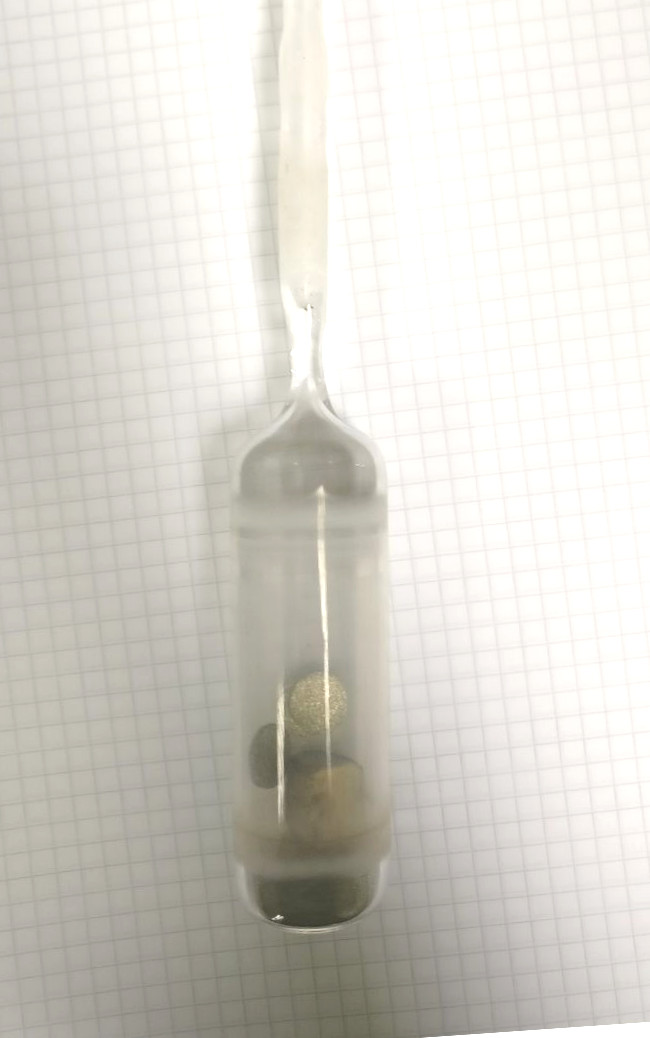
\includegraphics[width=\textwidth]{Img/Procedimiento/ampolla.jpg}
        \caption{}
        \label{fig:ampolla}
    \end{subfigure}
    \begin{subfigure}{0.2\textwidth}
        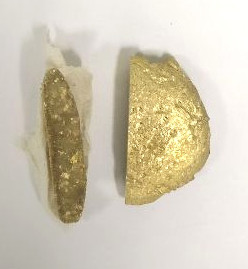
\includegraphics[width=\textwidth]{Img/Procedimiento/boton.jpg}
        \caption{}
        \label{fig:boton}
    \end{subfigure}
    \begin{subfigure}{0.2\textwidth}
        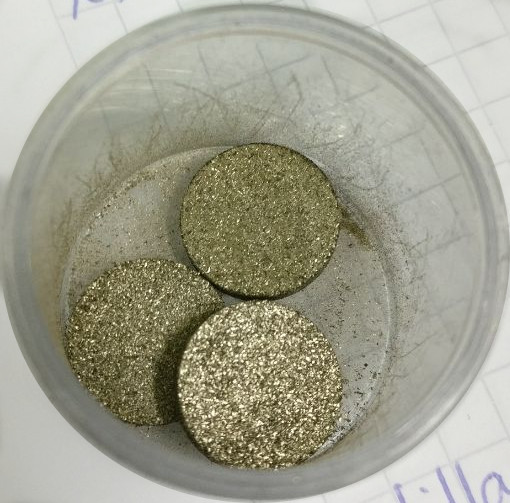
\includegraphics[width=\textwidth]{Img/Procedimiento/PastViruta.jpg}
	\caption{}. 
	\label{fig:PastViruta}
    \end{subfigure}
    ~ %add desired spacing between images, e. g. ~, \quad, \qquad, \hfill etc. 
      %(or a blank line to force the subfigure onto a new line)
    \begin{subfigure}{0.25\textwidth}
        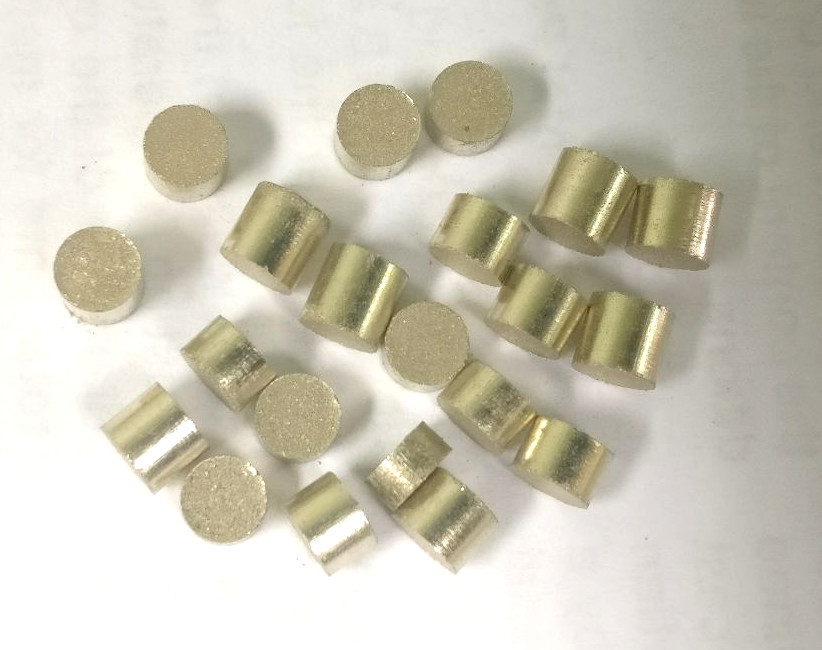
\includegraphics[width=\textwidth]{Img/Procedimiento/PastMolienda.jpg}
        \caption{}
        \label{fig:PastMolienda}
    \end{subfigure}
    \begin{subfigure}{0.1\textwidth}
        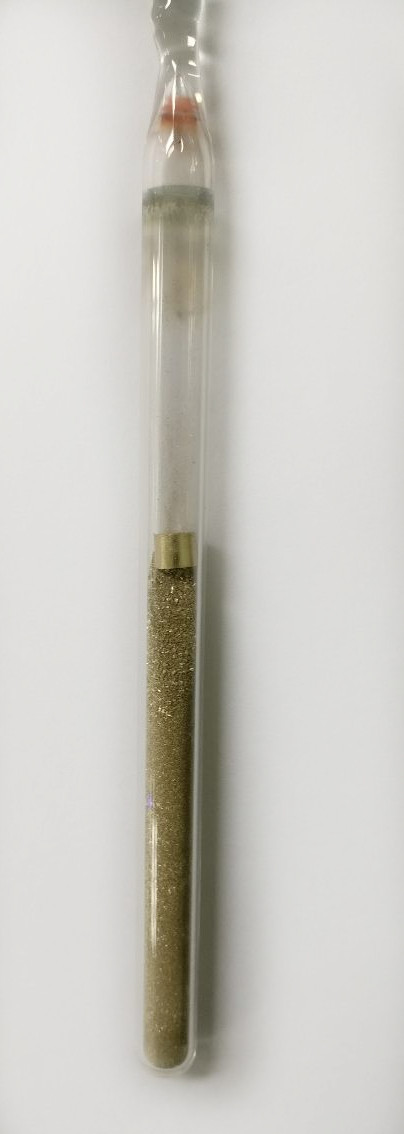
\includegraphics[width=\textwidth]{Img/Procedimiento/ClavoPolvo.jpg}
        \caption{}
        \label{fig:ClavoPolvo}
    \end{subfigure}
 \caption{Distintos métodos utilizados para refinar la estructura de la aleación de Cu-Zn-Al con polvo de $AlB_2$} 
    \end{figure}
    
    
    Una vez fabricados los distintos clavos, se emparejaron las superficies utilizando un equipo de electroerosión, obteniendo probetas cilíndricas que fueron ensayadas con distintos ciclos de compresión. La deformación se midió con un extensómetro marca Instrom y se siguió la misma metodología que se explica en la sección \ref{compresión}.
    

\section{Fabricación de esponjas} \label{FabricacionEsponjas}

A continuación se detalla el método utilizado para fabricar esponjas. El proceso puede verse en la figura \ref{fig:detalleproceso}. Se partió de un lingote de aleación de Cu-Zn-Al fabricado con el método descripto en la sección \ref{preparacion_aleacion}. Este lingote se colocó en un crisol de grafito, y se calentó hasta fundir en un horno de inducción. Una vez que la aleación se encontraba en estado líquido se colocaron encima las esferas de sílica gel previamente secadas en una estufa por varias horas para eliminar humedad que pueda haber absorbido del ambiente (figura \ref{fig:pro1}).

\begin{figure}[h]
 \centering
    \begin{subfigure}{0.2\textwidth}
        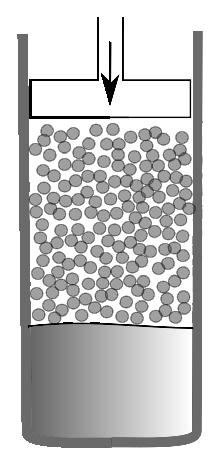
\includegraphics[width=\textwidth]{Img/Procedimiento/proceso1.eps}
        \caption{}
        \label{fig:pro1}
    \end{subfigure}
        \begin{subfigure}{0.05\textwidth}
        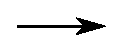
\includegraphics[width=\textwidth]{Img/Procedimiento/flecha.eps}
    \end{subfigure}
    \begin{subfigure}{0.2\textwidth}
        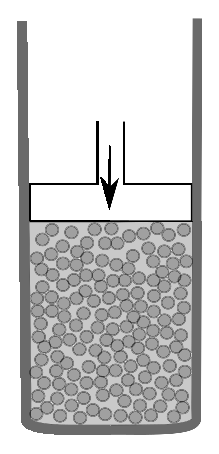
\includegraphics[width=\textwidth]{Img/Procedimiento/proceso2.eps}
        \caption{}
        \label{fig:pro2}
    \end{subfigure}
        \begin{subfigure}{0.05\textwidth}
        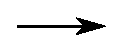
\includegraphics[width=\textwidth]{Img/Procedimiento/flecha.eps}
    \end{subfigure}
    \begin{subfigure}{0.2\textwidth}
        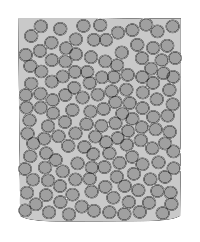
\includegraphics[width=\textwidth]{Img/Procedimiento/proceso3.eps}
        \caption{}
        \label{fig:pro3}
     \end{subfigure}
%             \begin{subfigure}{0.05\textwidth}
%         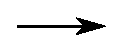
\includegraphics[width=\textwidth]{Img/Procedimiento/flecha.eps}
%     \end{subfigure}
%     \begin{subfigure}{0.1\textwidth}
%         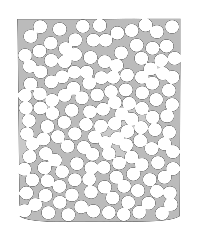
\includegraphics[width=\textwidth]{Img/Procedimiento/proceso4.eps}
%         \caption{}
%         \label{fig:pro3}
%     \end{subfigure}
  \caption{Distintas etapas en el proceso de fabricación de esponjas}
    \label{fig:detalleproceso}
\end{figure}

Estas esferas, que quedan flotando en la superficie del metal líquido, se presionaron con un pistón de manera que el metal líquido se infiltre entre las esferas (figura \ref{fig:pro2}). Como puede verse en la figura \ref{fig:proceso1} se obtuvo un lingote cilíndrico compuesto por las esferas de sílica gel y una matriz metálica.

Una vez enfriado, se torneó la muestra para retirar una fina capa superficial y se obtuvo una pieza como la que se ve en la la figura \ref{fig:proceso2}. Luego se colocó este cilindro en una solución de ácido fluorhídrico al $50\%$ (la cual ataca únicamente la sílica y no la aleación) y se dejó reposar durante tres días. Como las esferas de sílica gel generan una estructura celular abierta, las celdas se encuentran interconectadas, y el ácido puede penetrar en toda la estructura.  Para acelerar el proceso se puede renovar la solución de ácido ya que la misma se va neutralizando a medida que la reacción avanza. También se puede utilizar un agitador magnético que mantenga la solución fluyendo. Una vez que se observó que no había más sílica, se enjuagó con agua para quitar toda la solución de ácido que pueda quedar en el interior de la estructura.

Por último se cortaron los extremos y se desbastaron para asegurar que sean dos superficies perfectamente paralelas para luego poder realizar los
ensayos mecánicos correctamente. Si se desean obtener micrografías ópticas o con SEM, se puede atacar la esponja con ácido nítrico al $50\%$ para que la superficie quede libre de cualquier óxido o impurezas superficiales que puedan quedar de todo el proceso. Se obtuvo entonces la esponja como la que se muestra en la figura \ref{fig:proceso3}.


\begin{figure}[h]
 \centering
    \begin{subfigure}{0.30\textwidth}
        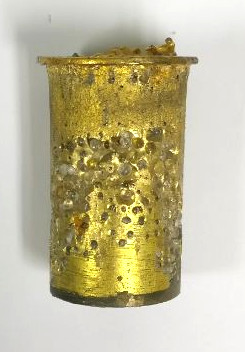
\includegraphics[width=\textwidth]{Img/Procedimiento/proceso1.jpg}
        \caption{Etapa I}
        \label{fig:proceso1}
    \end{subfigure}
    \begin{subfigure}{0.35\textwidth}
        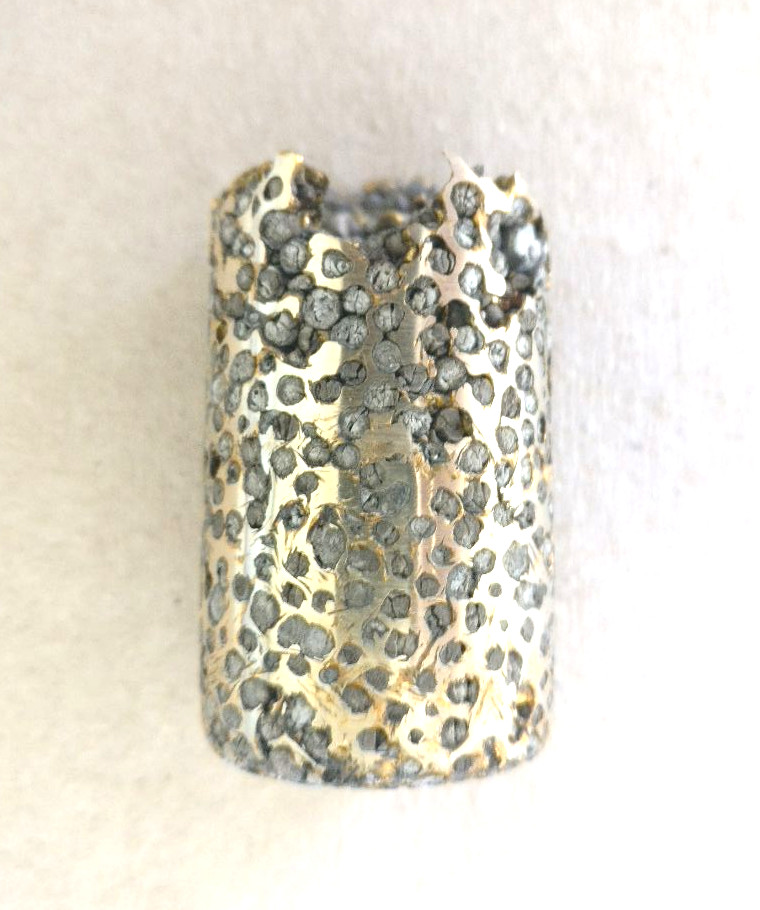
\includegraphics[width=\textwidth]{Img/Procedimiento/proceso2.jpg}
        \caption{Etapa II}
        \label{fig:proceso2}
    \end{subfigure}
    \begin{subfigure}{0.28\textwidth}
        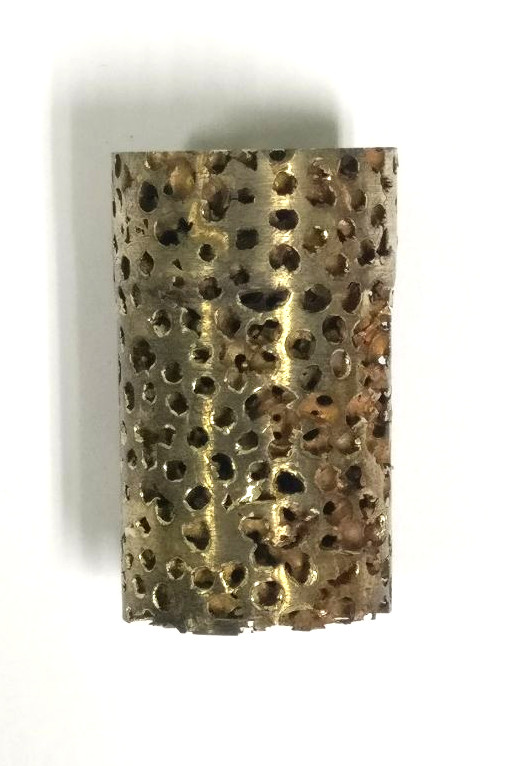
\includegraphics[width=\textwidth]{Img/Procedimiento/proceso3.jpg}
        \caption{Etapa III}
        \label{fig:proceso3}
    \end{subfigure}
  \label{fig: proceso}
  \caption{Distintas etapas en el proceso de fabricación de esponjas}
\end{figure}


\section{Caracterización y Ensayos}



\subsection{Medición de temperatura de transformación martensítica}

Para que la transformación martensítica avance y retroceda al aplicar y retirar cargas respectivamente,  se debe trabajar entre las temperaturas $M_s$ y $M_d$. Si se trabaja con una temperatura inferior a $M_s$, la aleación formará martensita estable al enfriarse. Por otro lado si se utilizan temperaturas muy altas, la martensita formada  por las tensiones mecánicas se estabilizará por un proceso de envejecimiento, y no ocurrirá una retransformación a austenita al retirar las cargas. Estos dos factores van en detrimento de las propiedades de memoria de forma, por lo que conocer la $M_s$ de la aleación es muy importante.

Debido a esto, previo a cada ensayo se realizó una medición de la temperatura de transformación martensítica del material de la muestra.
Para llevar a cabo las mediciones se soldó a la muestra una termocupla tipo K. La termocupla se conectó a una punta fría, y esta a su vez a un voltímetro que registraba las mediciones en una computadora. Con un termo con nitrógeno líquido y un calentador de laboratorio a 150 $^\circ C$  se realizaron rampas de calentamiento y enfriamiento. 
Como se muestra en el gráfico \ref{fig:Ms}, si se gráfica la velocidad de calentamiento o enfriamiento en función de la temperatura, se verá un pico a la temperatura que ocurra la transformación martensítica. Lo mismo sucederá en la transformación inversa de martensita a austenita. De esta forma se puede medir tanto la $M_s$ como la $A_s$.



\begin{figure}[h]
 \centering
 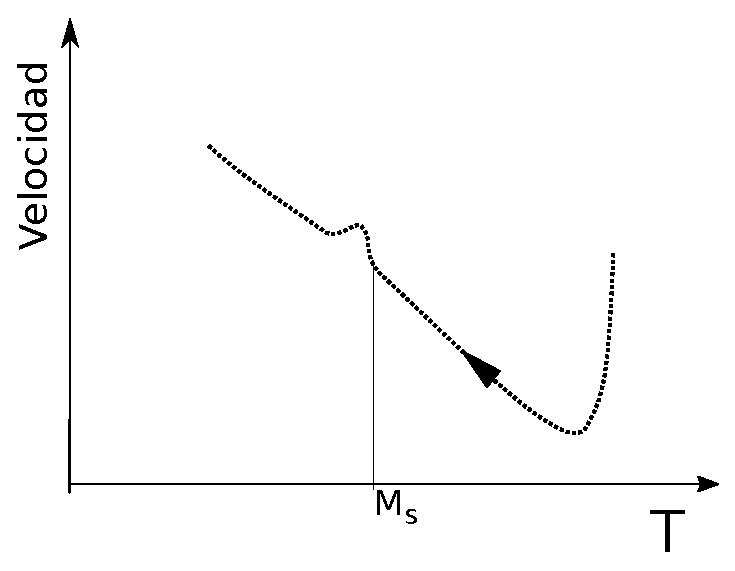
\includegraphics[width=0.5\textwidth]{Img/Procedimiento/Ms.eps}
 \caption{Esquema del gráfico obtenido en la medición de la $M_s$}. 
 \label{fig:Ms}
 \end{figure}


\subsection{Metalografía}

Al preparar las muestras para análisis metalográfico hay que tener en cuenta que la aleación transformará a martensita tanto por temperatura como por deformación. Por este motivo los cortes de muestras se realizaron utilizando una cortadora de precisión IsoMet, que genera deformación reducida ya que utiliza discos diamantados. También debe realizarse el desbaste y pulido con suavidad para que este no produzca una transformación 
martensítica en la superficie. Por otro lado hay que controlar que el agua utilizada para lavar las muestras no sea muy fría en el caso 
que la $M_s$ del material esté cercana a la temperatura ambiente. 

Generalmente se inicia el desbaste con una lija de carburo de silicio, empezando desde un granulado tamaño 400 y se va subiendo hasta un número 1000. 
Luego se realiza un pulido con alúmina de 1 $\mu m$. Finalmente se ataca durante unos $5$ segundos con una solución de $50 \% $ de ácido nítrico para revelar bordes de grano y la microestructura. 

Para las muestras que se analizaron en SEM, fue necesario un ataque con ácido nítrico durante una mayor cantidad de tiempo que el utilizado en las micrografías para que pueda distinguirse la rugosidad de la superficie generada por la microestructura.

\subsection{Respuesta mecánica a compresión} \label{compresión}

% Deformacion real e ingenieril

% https://books.google.com.ar/books?id=gilYI9_KKAoC&pg=PA60&lpg=PA60&dq=deformacion+real+e+ingenieril&source=bl&ots=mocOuVvrLx&sig=-0en3S3S9Pv8Ty2yMc08LHGR7zs&hl=en&sa=X&ved=0ahUKEwix953zr-DTAhUBgpAKHRsoAaMQ6AEIXjAK#v=onepage&q=deformacion%20real%20e%20ingenieril&f=false

Para ensayar esponjas, tanto de Cu-Zn-Al como de Cu puro, se procedió de la siguiente forma. Una vez fabricadas las esponjas como se explicó en la sección  \ref{FabricacionEsponjas}, se cortaron los bordes con una cortadora de precisión IsoMet y luego se desbastaron para que ambos extremos sean perfectamente planos y paralelos. Esto es muy importante para que al comprimir la deformación sea homogénea en toda la muestra y no se concentre, por ejemplo, en un costado. Previo al ensayo se realizó un recocido a 800 $^\circ C$ durante media hora y un enfriamiento al aire durante media hora más con el fin de reiniciar el estado termomecánico del material, esto es, para borrar cualquier rastro de martensita anterior y asegurar que todas las muestras empiecen con la misma estructura. 

Los ensayos se realizaron en una máquina de ensayos mecánicos Instron 1123. Se utilizó una jaula inversora que transforma el movimiento de tracción de las mordazas del equipo en compresión de la probeta, ya que con este equipo no puede realizarse ensayos de compresión directamente entre discos debido a la rótula que une la celda de carga con el resto de los elementos de la cadena cinemática. El equipo utilizado puede verse en la figura \ref{fig:jaula}. La 
temperatura de los ensayos se controló con una cámara ambiental Instron 
%TODO numero de la camara ambiental y del extensómetro
perteneciente a la máquina de tracción, la cual puede enfriar y calentar.
La deformación de la muestra se registró con un extensómetro marca Instron de $12,5 mm$ de longitud calibrada y una deformación de $\pm 12\%$ el cual se fija a la muestra utilizando combinaciones de 
resortes de distinta longitud dependiendo del diámetro de la muestra a ensayar. En el caso de la esponja de Cu, como se deformó hasta comprimirse 
completamente no fue posible utilizar el extensómetro, por lo que se registró la deformación a partir del movimiento de los cabezales de la máquina, y luego 
se graficó la deformación real de la muestra dada por la expresión \ref{defreal}

\begin{equation}
d \varepsilon = \frac{dl}{l}  \longrightarrow  \varepsilon =ln \left(\frac{l}{l_0}\right) \label{defreal} 
\end{equation}



Si bien el horno posee un controlador de temperatura, para tener una medición
más precisa de la temperatura de la muestra se utilizó una termocupla tipo K adherida a la superficie de la jaula de compresión.

\begin{figure}[h]
 \centering
 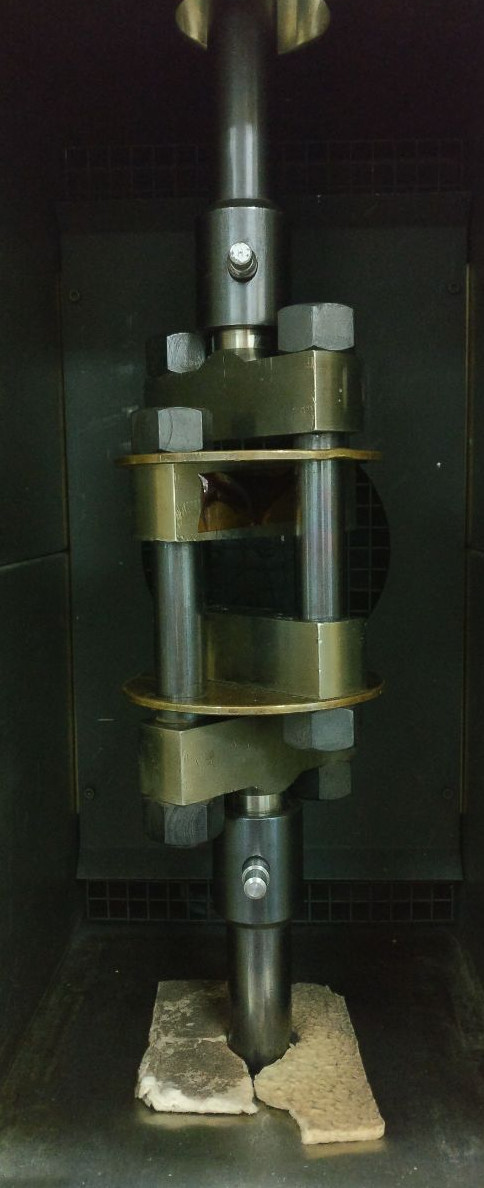
\includegraphics[width=0.2\textwidth]{Img/Procedimiento/jaula.jpg}
 \caption{Dispositivo de compresión utilizado en los ensayos} 
 \label{fig:jaula}
 \end{figure}

%  \begin{figure}[h]
%  \centering
%     \begin{subfigure}{0.70\textwidth}
%     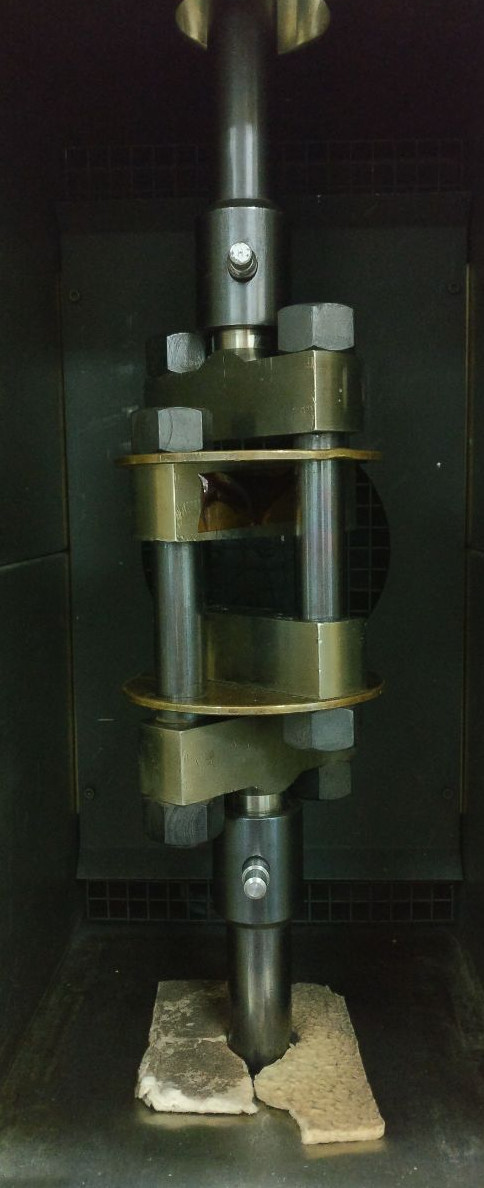
\includegraphics[width=0.2\textwidth]{Img/Procedimiento/jaula.jpg}
% % \caption{} 
%     \end{subfigure}
%     \begin{subfigure}{0.25\textwidth}
%         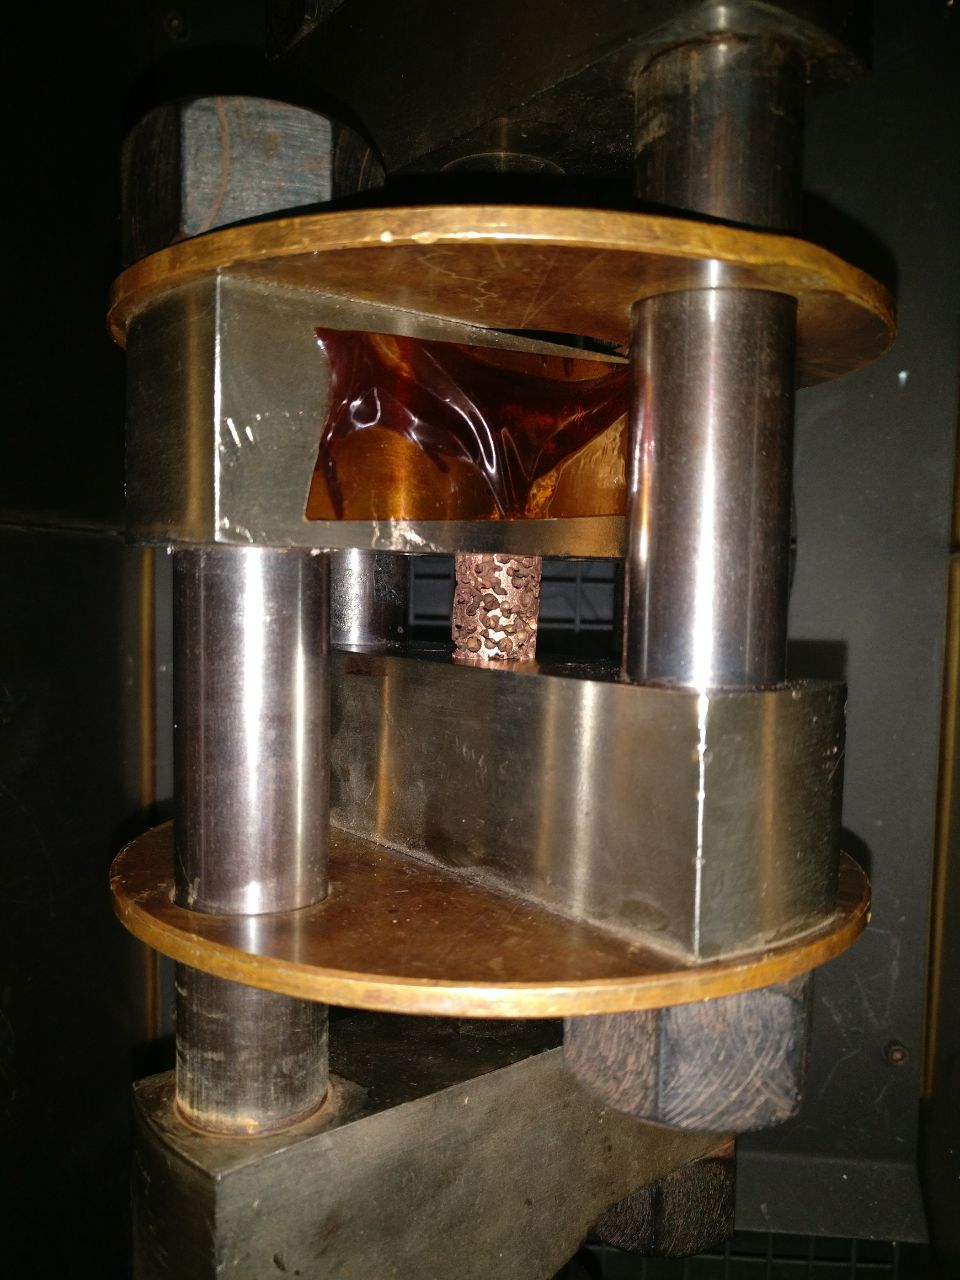
\includegraphics[width=\textwidth]{Img/Procedimiento/jaula2.jpg}
% %        \caption{}
%     \end{subfigure}
%   \caption{Dispositivo de compresión utilizado en los ensayos}
% \end{figure}
 

Para ensayar los clavos con distintos tamaños de grano, se procedió de manera muy similar. Primero se tornean los bordes con una cortadora por electro erosión. Esta máquina erosiona la superficie sin generar deformación en el material, y permite obtener cilindros con superficies muy parejas. Luego de emparejar las superficies, se cortaron las probetas de aproximadamente $25 mm$ de largo y se emparejaron las puntas para que queden perfectamente paralelas. 
Los ensayos de compresión se llevaron a cabo de la misma forma que las esponjas. 
 

\subsection{Resistencia} \label{CuatroPuntas}

% http://users.df.uba.ar/sgil/labo3_uba/guias/cuatro_punta2k6_l3.pdf

Para medir la resistencia de las muestras se utilizó el método de las cuatro puntas, también conocido como método de Kelvin. En la figura 
\ref{fig:CuatroPuntas} puede 
verse el dispositivo utilizado. A la muestra se le soldaron cuatro cables alineados, con los dos exteriores se le inyecta una corriente conocida y con los 
otros dos cables se mide la tensión en la muestra. Este método permite realizar mediciones de resistencias muy pequeños, ya que como varía
el sentido de la corriente permite eliminar los potenciales y resistencias que se generan en las soldaduras de los cables a la muestra.
Como el voltímetro que lee la tensión con los cables interiores posee una resistencia muy alta, podemos considerar que por este cable no circula una corriente
y entonces la medición de tensión será precisa. 

Si la corriente circula en un sentido, la tensión leída por el voltímetro será:
\begin{equation}
 V^+= V_A +I^+ . R - V_B 
\end{equation}
Donde $V_A$ y $V_B$ son los potenciales que se generan en las soldaduras de los cables a la muestra. Si ahora la corriente circula en sentido contrario la tensión leída será:
\begin{equation}
 V^-= V_A +I^- . R - V_B 
\end{equation}

El equipo registra entonces las tensiones con la corriente circulando en un sentido y en el otro. Si estas tensiones se restan, se cancelarán los potenciales 
de las soldaduras, quedando:  
\begin{equation}
 V^+ - V^-= [I^+ + I^-] R \longrightarrow R=\frac{V^+ - V^-}{(I^+ + I^-)}
\end{equation}

Sabiendo que la corriente aplicada es siempre 200 mA, y conociendo las dimensiones de las probetas utilizadas, se llega a la resistividad dada por la 
ecuación \ref{resist} la cual permite comparar los resultados de los distintos ensayos de distintas muestras, ya que normaliza los parámetros geométricos.

\begin{equation}
 \rho = R . \frac{A}{l} \label{resist} 
\end{equation}
Donde $\rho$ es la resistividad, $R$ es la resistencia medida de la probeta, $A$ es la sección y $l$ la longitud entre los cables que miden la tensión.

 
 
 \begin{figure}
    \centering
    \begin{subfigure}{0.4\textwidth}
        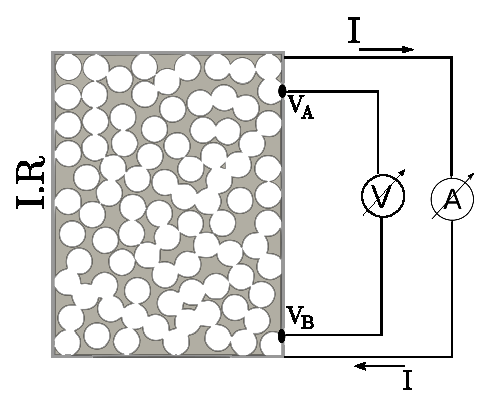
\includegraphics[width=\textwidth]{Img/Procedimiento/CuatroPuntas1.eps}
	\caption{Esquema del dispositivo}. 
	\label{fig:CuatroPuntas}
    \end{subfigure}
    ~ %add desired spacing between images, e. g. ~, \quad, \qquad, \hfill etc. 
      %(or a blank line to force the subfigure onto a new line)
    \begin{subfigure}{0.4\textwidth}
        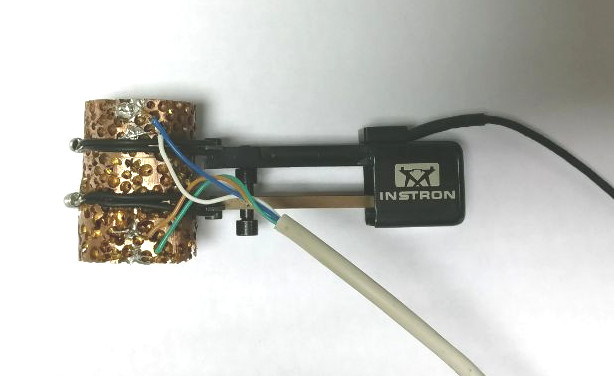
\includegraphics[width=\textwidth]{Img/Procedimiento/cpfoto.jpg}
        \caption{Foto del dispositivo utilizado}
        \label{fig:cuatropuntasyextensometro}
    \end{subfigure}
    \caption{Esquema y fotografía de la disposición de los cables en la muestra para medir la resistencia por el método de las cuatro puntas. }
\end{figure}


\begin{figure}[h]
 \centering
 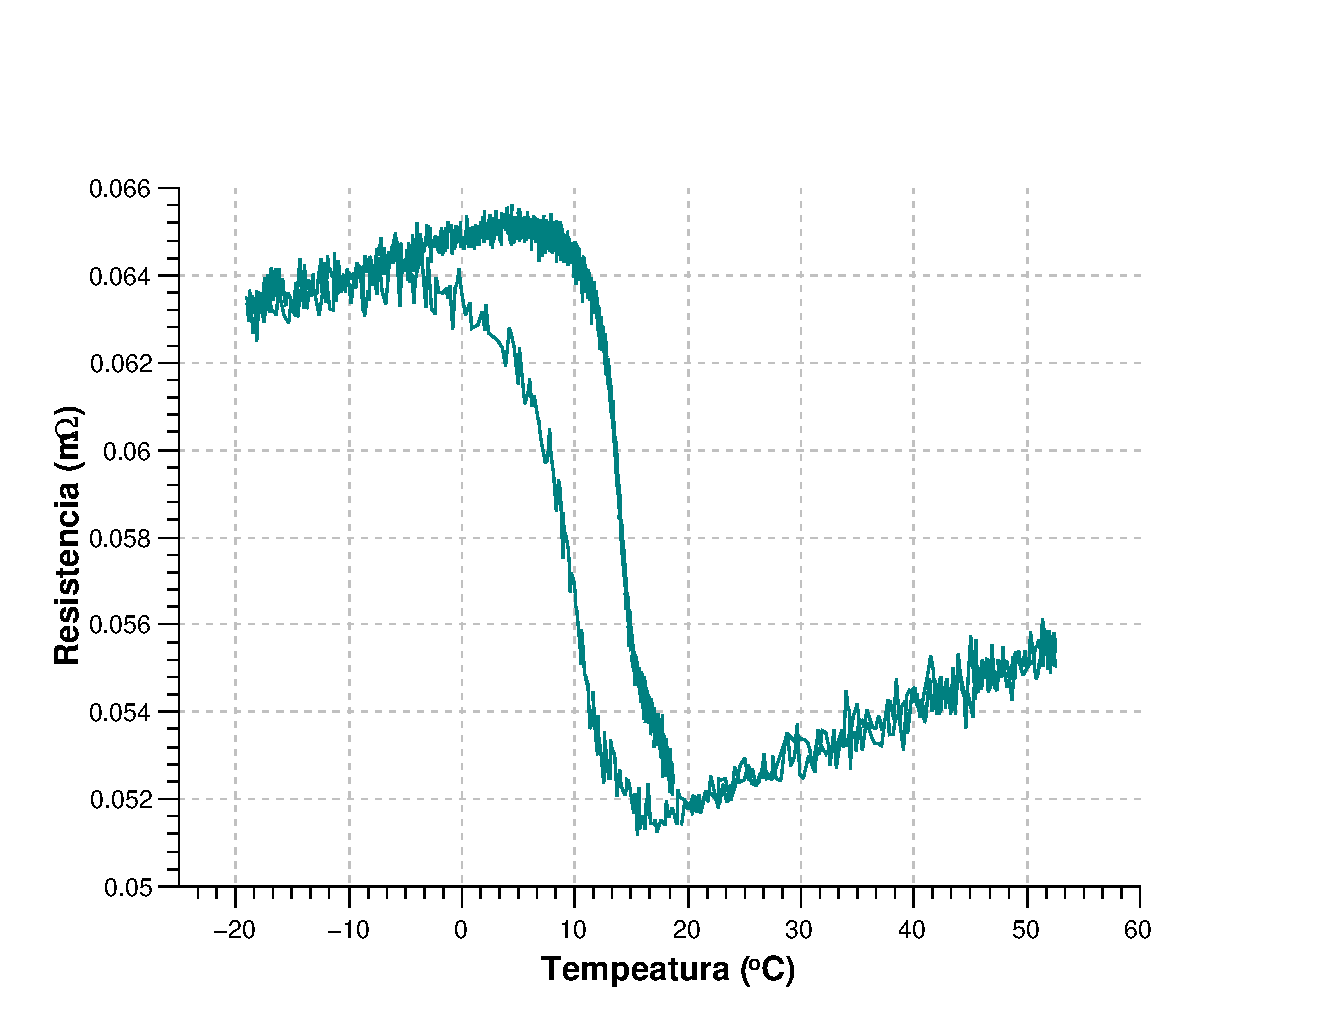
\includegraphics[width=0.5\textwidth]{Img/Resultados/RvsTClavo5.eps}
 \caption{Ejemplo de la variación de la resistencia en función de la temperatura al transformar en un ciclo de enfriamiento y calentamiento.} 
 \label{fig:RvsTClavo5}
 \end{figure}

En el gráfico \ref{fig:RvsTClavo5} puede verse la variación de la resistencia en un ciclo de enfriamiento y calentamiento, cuando transforma a martensita y austenita respectivamente. Puede verse que la martensita presenta una resistencia mucho mayor a la austenita. La medición de la resistencia a medida que transforma la aleación es muy útil, ya que permite seguir 
de manera detallada el avance de transformación. Si se conoce la resistencia inicial en estado austenítico, y el valor de la resistencia cuando la 
muestra se encuentra en estado completamente martensítico, puntos intermedios entre estos dos extremos darán información acerca de la fracción transformada.
También puede verse que cuando la aleación se encuentra en estado austenítico o martensítico la resistencia varía linealmente con la temperatura, como es 
de esperarse para cualquier aleación metálica. 

% 
% Se calcularon las variaciones en la resistencia debido al cambio de volumen al comprimir, y a la dilatación o compresión térmica. En ambos casos estas 
% variaciones son despreciables por lo que no se tomarán en cuenta. También se graficó la variación en la medición del extensómetro por cambios de 
% temperatura y también resultó despreciable por lo que tampoco serán utilizados. 


% ****************************************************************************************************************************************************
% ****************************************************************************************************************************************************
% ****************************************************************************************************************************************************

\chapter{Resultados y discusión}
\label{sec:resultados}


\section{Tamaño de grano}

En este capítulo se presentan los resultados obtenidos al aplicar distintos métodos para modificar el tamaño de grano. En la sección \ref{reduccion} se detallan las muestras fabricadas y los resultados obtenidos al intentar reducir el tamaño de grano. En la sección \ref{aumento} se presentan los resultados obtenidos al intentar generar un aumento el tamaño de grano de la aleación. Finalmente en la sección \ref{TamañosConclusion} se presentan las conclusiones a las que se llegaron en este capítulo y el trabajo que debe continuarse a futuro. 


\subsection{Reducción del tamaño de grano} \label{reduccion}

Como se explicó en la sección \ref{FabClavos}, se encontró en la bibliografía que el método más efectivo para refinar el tamaño de grano es la utilización de $B$ como refinador. En el trabajo realizado por Rit Elst \textit{et al.} \cite{ritelst} se obtuvo para unas concentraciones de boro entre $0.04$ y $0.06$ $\% pp$ un tamaño de grano entre $50$ y $100$ $\mu m$, y para $0.01$ $\%pp$ tamaños entre $1$ y $2$ $mm$. Estos tamaños se obtuvieron luego de fundir la aleación con el agregado de boro y un recocido a $750$ $^\circ C$ durante quince minutos seguido de un temple en agua. El boro reacciona con el aluminio de la aleación formando $AlB_2$ que es el compuesto responsable del efecto refinador. Como en el laboratorio se contaba con $AlB_2$ en forma de polvo se utilizó este compuesto directamente. 


\begin{table} 
\begin{center} 
\begin{tabular}{@{}lllll@{}} \toprule
Muestra & $wt \% AlB_2$ & Método de fabricación & $\bar{tg} (mm)$ & $\sigma$ \\ \midrule
 Clavo 5 &  -     & -   & 0.59  & 0.30   \\
 L1B1    &  0,005 & I   & 0.31 & 0.22  \\
 Clavo 1 &  0,5   & III & 0.16 & 0.08   \\
 Clavo 2 &  0,05  & III & 0.10 & 0.05   \\
 Clavo 3 &  -     & IV  & 0.11 & 0.05   \\
 Clavo 4 &  0,005 & IV  & 0.07 & 0.03   \\
\bottomrule
\end{tabular}
\caption{Porcentaje de polvo refinador, método de fabricación, valor medio del tamaño de grano ($\bar{tg}$) y desviación media de las distribuciones ($\sigma$) de las distintas muestras fabricadas.}
\label{tab:ResClavos}
\end{center}
\end{table}


En el cuadro \ref{tab:ResClavos} se muestra el valor medio de los tamaños de granos ($\bar{tg}$) que se obtuvieron en cada una de las muestras. El método de fabricación de cada muestra se detalló en la sección \ref{FabClavos}. También se muestra la desviación media de la distribución de tamaño de grano ($\sigma$). En el gráfico \ref{fig:tamaños} se esquematizan estos mismos resultados.

 \begin{figure}[h]
 \centering
 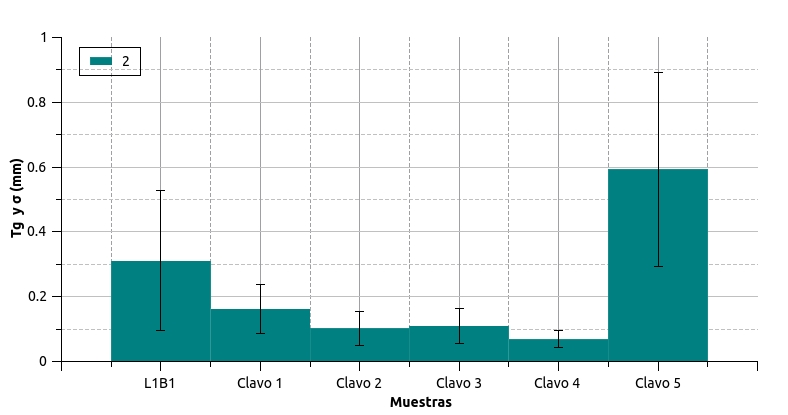
\includegraphics[width=0.9\textwidth]{Img/Resultados/clavos/TamGranos.jpg}
 \caption{Valor medio de tamaño de grano ($\bar{tg}$) y desviación media de la distribución ($\sigma$) de cada una de las muestras fabricadas} 
 \label{fig:tamaños}
 \end{figure}

A continuación se detallan los resultados obtenidos con cada una de las muestras. La nomenclatura utilizada corresponde a \textbf{L} para el lingote de aleación utilizado para fabricar la muestra y \textbf{B} cuando la muestra obtenida tiene geometría de botón. Los \textbf{Clavos} corresponden a muestras cilíndricas de $6$ mm de diámetro aproximadamente y una longitud que puede variar entre $30$ y $100$ mm.
 
 Las muestras \textbf{ L1B1} y \textbf{L1B2}, para las cuales se mezcló el polvo refinador y una porción de aleación, no incorporaron correctamente el $AlB_2$. Como resultado quedó un botón de la aleación rodeado por el polvo refinador suelto. Luego de realizar un corte transversal y el pulido de la superficie no se observó una disminución significativa del tamaño de grano. Además el tamaño de grano resultó con granos de hasta medio milímetro de diámetro en las dos muestras. En la figura \ref{fig:MicroL1B1} se muestran micrografías de la muestra L1B1 tomadas por microscopía SEM.  

%***************************************************** graficos
  \begin{figure}% \label{fig:Clavo1}
    \centering
    
    ~ %add desired spacing between images, e. g. ~, \quad, \qquad, \hfill etc. 
      %(or a blank line to force the subfigure onto a new line)
    \begin{subfigure}{0.4\textwidth}
        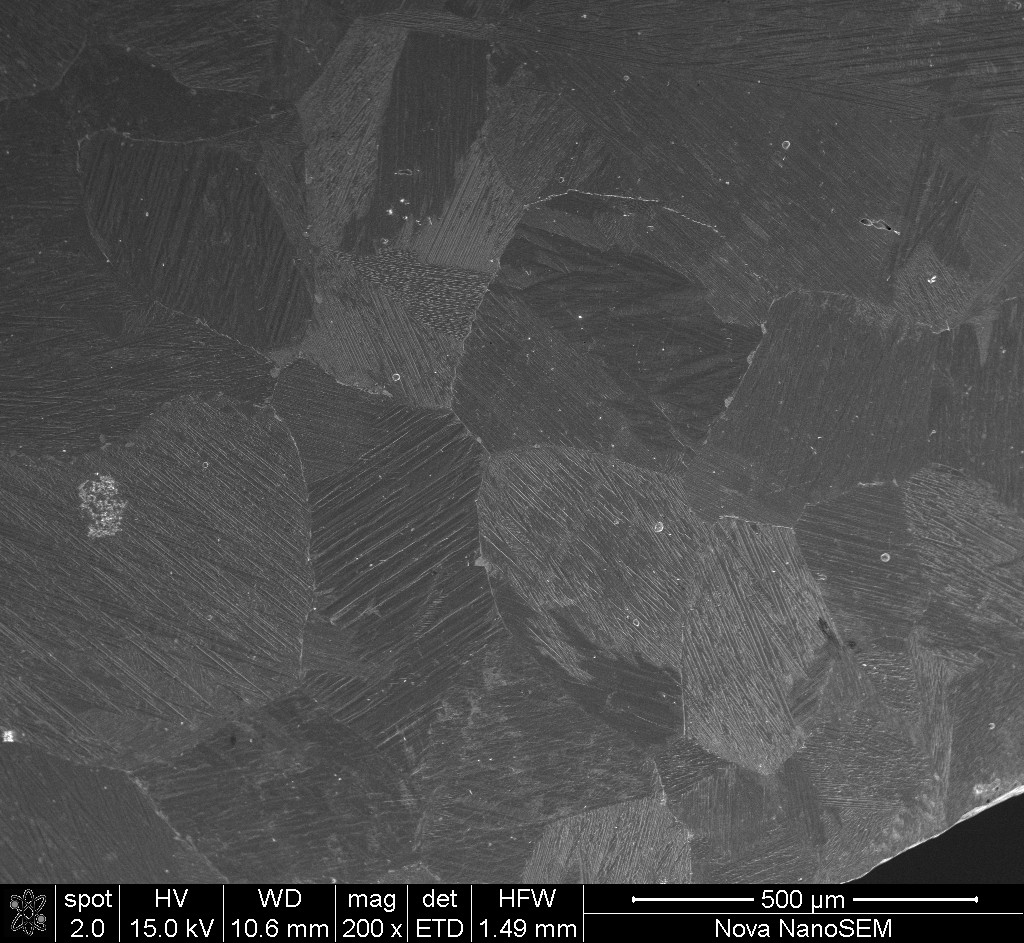
\includegraphics[width=\textwidth]{Img/Resultados/clavos/L1B1_016.jpg}
        \caption{}
        \label{fig:ExpRes}
    \end{subfigure}
    \begin{subfigure}{0.4\textwidth}
        \includegraphics[width=\textwidth]{Img/Resultados/clavos/L1B1_014.jpg}
        \caption{}
        \label{fig:ExpStrain}
    \end{subfigure}
    \caption{Micrografías tomadas por microscopía SEM del botón L1B1. En (a) se distinguen los granos de la aleación y placas de martensita, en (b) se muestra un aumento de las placas. El tamaño de grano es bastante grande y no se observan en la aleación partículas de $AlB_2$.}
    \label{fig:MicroL1B1}
    \end{figure}
 
 El botón \textbf{L2B1} se fabricó fundiendo pastillas de viruta de aleación y polvo de $AlB_2$ prensado. Además, se utilizó cien veces más cantidad de polvo refinador para intentar incorporarlo más fácilmente. Se observó que la aleación escurrió, formando un botón como los citados anteriormente, y junto al botón quedaron las pastillas conteniendo todo el polvo refinador y prácticamente nada de la viruta de aleación. El botón presentó el mismo tamaño de grano que las muestras \textbf{ L1B1} y \textbf{L1B2}.

El botón \textbf{L2B2} se fabricó de la misma manera que el botón \textbf{L2B1}. La única diferencia en el procedimiento fue que la temperatura utilizada para fundir se controló para no llegar a la transformación $AlB_2 \rightarrow AlB_{12}$, en caso de que esta transformación tuviera algún efecto en la incorporación del refinador. Nuevamente el refinador no fue incorporado y no se vio una reducción significativa del tamaño de grano. También se realizó un corte del botón y se analizó con microscopía SEM para ver si se encontraba alguna partícula de $AlB_2$. No se encontró refinador en las micrografías por lo que se corroboró que el polvo refinador no fue incorporado por la aleación. Las únicas partículas que se encontraron fueron pequeños precipitados que seguramente corresponden a una fase rica en zinc.


Viendo estos resultados se concluyó que el refinador no puede incorporarse de manera sencilla a la aleación. Por este motivo se realizó la molienda en un molino de bolas de la aleación junto al polvo refinador para favorecer la incorporación por la mezcla, y además un refinamiento del $AlB_2$. Se analizó el polvo obtenido en la molienda con microscopia SEM y EDS. Se realizaron análisis de topografía y de composición con electrones retrodispersados pero no fue posible identificar partículas del polvo refinador. 



Luego se fabricó el \textbf{Clavo 1}. Se prensaron pastillas con el polvo obtenido de la molienda (Figura \ref{fig:PastMolienda}). Como se muestra en la figura \ref{fig: Clavo1}, al fundirlas se observó nuevamente que la aleación escurrió, quedando las pastillas con el polvo refinador y el metal escurrido en la superficie. Se hizo un corte transversal al clavo, y en la zona donde había escurrido la aleación se observaron los granos, los cuales presentaron el primer refinamiento marcado del tamaño de grano (Figura \ref{fig: MicroClavo1}). Además, si bien hay tamaños de grano variados, el ancho de la distribución también disminuyó.  Se distinguen las pastillas con refinador y la aleación que escurrió envolviendo las pastillas. En la figura \ref{fig: MicroClavo1} se ve un corte transversal del \textbf{Clavo 1}. En la parte izquierda se observa la geometría de la pastilla compuesta principalmente por el polvo refinador y muy pocos granos pequeños de la aleación. A la derecha se distingue claramente la aleación que quedó envolviendo las pastillas. En la figura \ref{fig: SEM1Clavo1} se muestra una imagen tomada con un microscopio electrónico de barrido (SEM) usando electrones retrodispersados donde se distingue la diferencia en la composición de la aleación y la zona donde quedó acumulado el polvo refinador. Los granos de aleación se ven más claros ya que poseen mayor cantidad de Cu y Zn, elementos de mayor número atómico. Por otro lado la zona con el polvo refinador se ve más oscura ya que posee una mayor concentración de Al y B, elementos de menor número atómico. También se realizó un análisis de Espectroscopia dispersiva en energía (EDS) para corroborar las composiciones en cada zona. En la figura \ref{fig: Sem2Clavo1} se ven los granos de la aleación y se distinguen partículas del polvo refinador que quedaron distribuidos en la aleación (pequeños puntos negros). Los círculos más grandes son pequeños poros que luego aumentaron su tamaño al realizar el pulido químico con ácido nítrico al $50 \%$.



 \begin{figure}[h]
 \centering
 \includegraphics[width=0.5\textwidth]{Img/Resultados/clavos/Clavo1_Foto2.jpg}
 \caption{Foto del \textbf{Clavo 1} luego de fundir las pastillas de aleación y refinador compactado} 
 \label{fig: Clavo1}
 \end{figure}




  \begin{figure}% \label{fig:Clavo1}
    \centering
    
    ~ %add desired spacing between images, e. g. ~, \quad, \qquad, \hfill etc. 
      %(or a blank line to force the subfigure onto a new line)
    \begin{subfigure}{0.35\textwidth}
        \includegraphics[width=\textwidth]{Img/Resultados/clavos/Clavo1.jpg}
        \caption{}%Corte transversal del Clavo 1}
        \label{fig: MicroClavo1}
    \end{subfigure}
        \begin{subfigure}{0.3\textwidth}
        \includegraphics[width=\textwidth]{Img/Resultados/clavos/Clavo1Retro.jpg}
        \caption{}%Corte transversal del Clavo 1}
        \label{fig: SEM1Clavo1}
    \end{subfigure}
        \begin{subfigure}{0.3\textwidth}
        \includegraphics[width=\textwidth]{Img/Resultados/clavos/Clavo1Retro2.jpg}
        \caption{}%Corte transversal del Clavo 1}
        \label{fig: Sem2Clavo1}
    \end{subfigure}
    \caption{Micrografías de un corte del Clavo 1: (a) Micrografía obtenida por microscopia óptica, En la figura $(b)$ y $(c)$ se muestran dos imágenes tomadas con un microscopio SEM con electrones retrodispersados donde se distingue la diferencia en la composición de la aleación (zonas grises) y la zona donde quedó acumulado el polvo refinador (en negro). En la figura $(c)$ se ven los granos de la aleación y se distinguen partículas del polvo refinador que quedaron distribuidas en la aleación. Los círculos más grandes son pequeños poros que luego aumentaron su tamaño al realizar el pulido químico.}
    \end{figure}

Luego de los resultados obtenidos con el \textbf{Clavo 1}, se fabricó el \textbf{Clavo 2} siguiendo la misma metodología, pero esta vez se utilizó una cantidad diez veces menor de polvo refinador ($0.05\%$ en peso). Luego de fundir, nuevamente quedaron las pastillas (esta vez con menos polvo) y el metal escurrió hacia el exterior. Además de perder la aleación, las superficies en las que hacen contacto las pastillas no se adhirieron correctamente, quedando como un punto muy débil en la estructura muy propenso a fisuras. Nuevamente se observó un refinamiento de la estructura en los lugares donde la aleación escurrió (Figura \ref{fig: MClavo2}).

A partir de los resultados obtenidos hasta esta instancia se concluyó que no es favorable realizar el prensado del polvo de la molienda en pastillas. 
%Como el \textbf{Clavo 2}, el cual tiene diez veces menos refinador que el \textbf{Clavo 1}, pero presenta un menor tamaño de grano, 
Luego se fabricó el \textbf{Clavo 3} de la siguiente forma. Esta muestra consistió únicamente en la molienda de la aleación, sin el agregado de polvo refinador. Además el polvo obtenido de la molienda se colocó suelto en el tubo de cuarzo. Se obtuvo un clavo como los anteriores, y también presentó un tamaño de grano pequeño similar a los \textbf{Clavos 1} y \textbf{2} (Figura \ref{fig: MClavo3}). Se concluyó que este refinamiento se debe a la formación de óxidos en la fabricación de la viruta de la aleación y posterior molienda en el molino de bolas. El único defecto que se encontró en esta muestra es la presencia de porosidad, que puede deberse a la baja densidad del polvo en el tubo de cuarzo, que no se compacta adecuadamente al fundirse. Además se ven en algunas zonas manchas de un tono un poco más oscuras al tono que presenta el resto de la muestra, que se deben a la aglomeración de óxidos. Estas manchas pueden actuar como una zona con tendencia a fisurarse cuando se someta la muestra a ensayos mecánicos. 

Por último, se fabricó el  \textbf{Clavo 4}, con $0.005 \%$ en peso de refinador (la menor cantidad de refinador utilizada hasta el momento). Además el polvo refinador se colocó suelto en el tubo de cuarzo al igual que en el \textbf{Clavo 3}. Se obtuvo el menor tamaño de grano y también la distribución mas estrecha (Figura \ref{fig: MClavo4}). Al igual que en el \textbf{Clavo 3}, la muestra presentaba porosidad y algunas manchas que pueden deberse a la aglomeración de óxido y también partículas de $AlB_2$.
 


Todas estas muestras se compararon con un clavo fabricado anteriormente por el grupo de investigación. Esta muestra, que llamamos \textbf{Clavo 5}, fue fabricada únicamente fundiendo la aleación, sin un proceso de molienda ni el agregado de $AlB_2$. Como se ve en el Cuadro \ref{tab:ResClavos} es la muestra con el mayor tamaño de grano y el mayor ancho de distribución. De esta forma puede verse que en las muestras \textbf{Clavo 3} y \textbf{Clavo 4} se obtuvo una considerable mejora.   



  \begin{figure}% \label{fig:Clavo1}
    \centering
    
    ~ %add desired spacing between images, e. g. ~, \quad, \qquad, \hfill etc. 
      %(or a blank line to force the subfigure onto a new line)
    \begin{subfigure}{0.3\textwidth}
        \includegraphics[width=\textwidth]{Img/Resultados/clavos/tg/Clavo1.jpg}
        \caption{Corte transversal del Clavo 1}%Corte transversal del Clavo 1}
        \label{fig: MClavo1}
    \end{subfigure}
        \begin{subfigure}{0.3\textwidth}
        \includegraphics[width=\textwidth]{Img/Resultados/clavos/tg/Clavo2.jpg}
        \caption{Corte transversal del Clavo 2}%Corte transversal del Clavo 1}
        \label{fig: MClavo2}
    \end{subfigure}
    \newline
    \centering
        \begin{subfigure}{0.3\textwidth}
        \includegraphics[width=\textwidth]{Img/Resultados/clavos/tg/Clavo3.jpg}
        \caption{Corte transversal del Clavo 3}%Corte transversal del Clavo 1}
        \label{fig: MClavo3}
    \end{subfigure}
        \begin{subfigure}{0.3\textwidth}
        \includegraphics[width=\textwidth]{Img/Resultados/clavos/tg/Clavo4.jpg}
        \caption{Corte transversal del Clavo 4}%Corte transversal del Clavo 1}
        \label{fig: MClavo4}
    \end{subfigure}    
    \caption{Corte transversal de los distintos clavos fabricados }
    \end{figure}

 \begin{figure}[h]
 \centering
 \includegraphics[width=0.9\textwidth]{Img/Resultados/clavos/Clavos_3_4_5.eps}
 \caption{Ciclos de compresión hasta distintos porcentajes de deformación de las diferentes muestras  } 
 \label{fig: Clavos3y4}
 \end{figure}







A partir de los clavos fabricados se cortaron probetas cilíndricas por electroerosión siguiendo el procedimiento descripto en la sección \ref{compresión}. Con estas probetas se realizaron distintos ciclos de compresión para analizar la incidencia de la estructura en el comportamiento mecánico. En los \textbf{Clavos 1} y \textbf{2}, la unión entre pastillas es muy débil, lo que provocó que las probetas se pandearan y quebraran. Por este motivo no fue posible realizar los ensayos de compresión. En el gráfico \ref{fig: Clavos3y4} se muestran los ciclos de deformación de los \textbf{Clavos 3}, \textbf{4} y \textbf{5}. Puede verse que el \textbf{Clavo 5} presenta una mayor recuperación de deformación en los ciclos que llegan a $1$ y $2 \%$. En los ciclos de mayor deformación el comportamiento se va igualando entre los \textbf{Clavos 3} y \textbf{4}.

Todos los ensayos se realizaron a una temperatura $40$ $^\circ C$ por encima de la $M_s$ de cada muestra, con excepción del clavo 4 que se utilizó $46$ $^\circ C$ por encima de su $M_s$. A partir de la ecuación de Clausius Clapeyron las tensiones de transformación deberían ser iguales en los casos en que el $\Delta T$ es el mismo (\textbf{Clavo 3} y \textbf{5}). Puede verse que el \textbf{Clavo 5} transforma a menores tensiones y la pendiente de la zona de transformación es la menor. Esto se debe a que la estructura contiene granos grandes y pocos defectos, lo que facilita la formación y crecimiento de las agujas de martensita. Al comparar los \textbf{Clavos 3} y \textbf{4} puede verse que el \textbf{Clavo 3} transforma a mayores tensiones, lo cual puede deberse a una mayor cantidad de partículas de óxido que también actúan como barrera para el avance de la transformación.  

   




\subsection{Aumento del tamaño de grano} \label{aumento}


Para comparar los resultados de una esponja con un tamaño de grano reducido, también se intentó obtener una esponja con un tamaño de grano mayor al que se obtiene al finalizar el proceso de fabricación. Para esto se tomó una esponja ya fabricada con las esferas de sílica gel en su estructura (figura \ref{fig:proceso2}). Se colocó en una ampolla de cuarzo con atmósfera de argón de un diámetro  $1 mm$ mayor al de la esponja. Luego se fue fundiendo la esponja con el método utilizado para crecer monocristales, llamado método de Bridgman. El método consiste en colocar una semilla, que le dará a la muestra la orientación cristalina deseada. Se produce en una muestra ya solidificada un gradiente térmico que recorre de una punta a la otra, fundiendo localmente, lo que provoca que la aleación fundida vaya solidificando a medida que se enfría con la orientación de la estructura de la semilla. Cuando la zona fundida recorrió toda la muestra, la probeta habrá solidificado con la misma orientación cristalográfica.

 \begin{figure}[h]
 \centering
 \includegraphics[width=0.5\textwidth]{Img/Resultados/EspRota.jpg}
 \caption{Foto del interior de una esponja que se rompió luego de intentar aumentar su tamaño de grano utilizando el método para solidificar monocristales de Bridgman.} 
 \label{fig: EspRota}
 \end{figure}

Para generar un aumento en el tamaño de grano se utilizó este mismo método. Aunque la presencia de las esferas de sílica gel actúa como puntos de nucleación, y además la geometría de la muestra no permite que solidifique como un único cristal, al utilizar este método se buscaba que el material que se iba fundiendo localmente solidifique con un tamaño de grano mayor al que se obtiene en la fabricación convencional de esponjas.

Una vez finalizado con el proceso se abrió la ampolla de cuarto y se encontró la presencia de una gran cantidad de vapor de ácido sulfhídrico. Se analizó el proceso de fabricación de las esferas de sílica gel para intentar determinar su procedencia. Las esferas de sílica gel están compuestas por una estructura porosa de óxido de silicio y su alta porosidad es lo que le da la capacidad de absorber la humedad. En algunos casos se le agrega cloruro de cobalto para obtener el efecto de cambio de color entre las esferas secas y con humedad en su interior. Se llegó a la conclusión que el azufre puede provenir de dos fuentes. La sílica gel se fabrica a partir de la neutralización de ácido sulfúrico y silicato de sodio. Si la reacción es incompleta pueden quedar rastros de azufre en las esferas. Por otro lado un subproducto de la reacción es el sulfato de sodio, que a altas temperaturas puede reaccionar con el cobre de la aleación, y a través de una reacción redox también  forma ácido sulfúrico. 

Luego se intentaron tornear las caras con un torno mecánico, pero al hacerlo la esponja se rompió como se muestra en la figura \ref{fig: EspRota}. En el interior se vio que la estructura estaba muy deteriorada y ya no tenía integridad suficiente para seguir utilizándola. Como la sílica que se utiliza en este método de fabricación de esponjas es comercial y no se puede tener certeza del grado de pureza en la composición de las esferas de sílica gel utilizadas, se concluyó que no es posible utilizar un método en la que se caliente las esferas a tan alta temperatura en una ampolla cerrada. 




% 
% A partir de este resultado se molieron $50 g$ de aleación con un $0.005\%$ en peso de $AlB_2$, en tandas de $8 g $. Una vez obtenidos $50 g$ de polvo, se fundió en una ampolla de cuarzo y atmósfera de argón, obteniéndose un pequeño lingote. Se realizó un corte transversal y se pulió para analizar el tamaño de grano.




% 
% 
% \section{Variación de Resistencia por deformación en Cu}
% 
% En el gráfico \ref{fig:ResDefCu} puede verse en rojo la variación teórica de la resistencia a medida que la probeta de Cu se comprime y varía su volumen (por el módulo de Poisson).
% En azul la medición de la resistencia al comprimir la probeta. Puede verse que la pendiente de la curva teórica es mayor. Esta diferencia puede deberse 
% al aumento de la resistencia debido a la deformación plástica lo que genera una pendiente bastante menor.
% 
% De todas formas las pendientes de estas curvas es muy chica, y despreciable al compararlas con la variación de la resistencia con la temperatura tanto en Austenita 
% como en Martensita. Por este motivo lo despreciamos al trabajar en ciclos térmicos.
% 
% \begin{figure}[h]
%  \centering
%  \includegraphics[width=0.8\textwidth]{Img/Resultados/ResDefCu.eps}
%  \caption{Variación de la resistencia de una probeta de Cu en función de la deformación a temperatura ambiente. En rojo el valor teórico correspondiente únicamente a la resistencia por cambio de volumen. 
%  En azul el valor medido de resistencia para cada porcentaje de deformación}. 
%  \label{fig:ResDefCu}
%  \end{figure}

\subsection{Discusión} \label{TamañosConclusion}

Respecto del método de fabricación, se comprobó que las concentraciones de refinador utilizadas en el trabajo de Rit Elst \textit{et al.} \cite{ritelst} son efectivas para obtener una disminución importante del tamaño de grano. Además queda en evidencia que la incorporación del refinador no es sencilla. Hay que aclarar que en el trabajo Rit Elst presenta los tamaños de grano que obtuvo, pero no indica si el polvo refinador fue incorporado totalmente o si se encontró con la misma dificultad. Además se concluyó que la molienda mecánica de la aleación con el refinador es efectiva para la incorporación, aunque no así el prensado de pastillas antes de realizar la fundición. También se demostró el efecto refinador observado por la presencia de óxido formado en las distintas etapas del proceso. Este óxido es el responsable de que en este trabajo se hay obtenido un tamaño de grano igual al de Rit Elst habiendo usado una cantidad de refinador mucho menor. Este óxido es prácticamente imposible de evitar a menos que se trabaje con atmósfera de argón desde los primeros cortes de la aleación, la molienda y posterior fundición. También queda por resolver la porosidad encontrada al fundir el polvo suelto en el tubo de cuarzo. Seguramente se necesitará alguna compactación para evitar esta porosidad, pero mucho menor a la compactación utilizada en la fabricación de las pastillas.

Para el aumento de tamaño de grano se demostró que los procesos que se realicen a alta temperatura en ampollas cerradas, deben realizarse cuando se tenga cierta precisión en la composición de las esferas de sílica gel. El hecho de que sea un material comercial, que no garantice cierto nivel de pureza y que por ejemplo contenga contaminación del proceso de fabricación, hace que se formen gases dentro de la ampolla, lo cual puede llevar a la degradación de la estructura. 

Respecto de las características de las aleaciones obtenidas, el \textbf{Clavo 5},que presenta el mayor tamaño de grano, es el que posee las mejores propiedades de memoria de forma. Luego de cada ciclo de deformación, el porcentaje de deformación recuperado es mayor que en los otros clavos con menor tamaño de grano. Además las tensiones de transformación son menores. Este resultado era esperado, ya que tener un mayor tamaño de grano permite el movimiento más libre de las interfases entre las placas de martensita y la austenita, ya que es una estructura con menor cantidad de bordes de grano y menos barreras como el polvo refinador y las partículas de óxido. Igualmente los requerimientos mecánicos de las esponja hacen que este refinamiento de grano sea necesario. En la figura \ref{fig: Fisuras} se muestra una macrografía donde se muestras varias fisuras intergranulares en una esponja que se sometió a distintos ciclos de deformación.

%  \begin{figure}[h]
%  \centering
%  \includegraphics[width=0.7\textwidth]{Img/Fisuras.eps}
%  \caption{Macrografía donde se señalan distintas fisuras intergranulares que se produjeron en una esponja que se sometió a numerosos ciclos de defomación.} 
%  \label{fig: Fisuras}
%  \end{figure}
 
    \begin{figure}% \label{fig:Clavo1}
    \centering
    
    ~ %add desired spacing between images, e. g. ~, \quad, \qquad, \hfill etc. 
      %(or a blank line to force the subfigure onto a new line)
     \begin{subfigure}{0.35\textwidth}
        \includegraphics[width=\textwidth]{Img/Esponjacompleta1.eps}
        \caption{}
        \label{fig:EsponjaCompleta1}
    \end{subfigure}
 \begin{subfigure}{0.45\textwidth}
        \includegraphics[width=\textwidth]{Img/Fisuras.eps}
        \caption{}
        \label{fig:Ciclos}
    \end{subfigure}
    \caption{Macrografías donde se señalan distintas fisuras intergranulares que se produjeron en una esponja que se sometió a numerosos ciclos de defomación.}
    \label{fig:Fisuras}
    \end{figure}
 

A partir de los resultados obtenidos se concluyó que el método óptimo para refinar el tamaño de grano es la utilización de una pequeña cantidad de $AlB_2$ como refinador ($0.005 \%$ pp es suficiente), el cual debe ser incorporado a través de una molienda mecánica. Si bien se obtuvo un tamaño de grano similar al utilizar únicamente la molienda mecánica de la aleación sin el agregado de polvo refinador, se recomienda utilizar una pequeña fracción de $AlB_2$ ya que el proceso de fabricación de las esponjas requerirá varias fundiciones, y la utilización de una pequeña cantidad de refinador ayudará a garantizar que no se produzca un aumento del tamaño de grano con cada aumento de la temperatura.


\section{Evaluación por resistividad de la integridad estructural}


Una aplicación donde se utilizan aleaciones con memoria de forma son los amortiguadores, ya que se aprovechan las propiedades pseudoelásticas de estos materiales. Por ejemplo, se podría colocar una esponja debajo de una mesa para que esta absorba las vibraciones. Cada vibración actuará como un ciclo de carga y descarga en la esponja. 
La carga oscilará entre el peso del equipo que se encuentra sobre la mesa y las cargas mayores generadas por las vibraciones.
Con cada ciclo de carga, la histéresis en la curva estará relacionada a la energía absorbida.  

Con las cargas más bajas la esponja tendrá una cantidad determinada de martensita y aumentará en cada nuevo ciclo de carga. Idealmente con cada ciclo de descarga la martensita retransformará a austenita volviendo al estado inicial. En la realidad esto no ocurre, ya que en cada ciclo se irá acumulando una pequeña cantidad de martensita retenida que se haya estabilizado, o por defectos en la estructura que dificultan el movimiento de las placas. Por otro lado, cada grano de la aleación tiene orientaciones cristalográficas distintas. La tensión resuelta es distinta en cada grano, por lo que cuando comienzan a transformar los primeros granos, los granos que aún no han transformado y no puedan acomodarse a la deformación del grano contiguo podrían provocar fisuras intergranulares. Sin mencionar que las mismas cargas pueden producir fisuras en los puntos más débiles de la estructura. 

Un posible método para analizar la integridad de una esponja es por tomografía, ya que permite ver en detalle el interior de la estructura. Pero es un método  que no puede realizarse in situ, sin sacar de funcionamiento el dispositivo, y requiere el uso de equipos complejos y costosos. Sería de gran utilidad poder monitorear la integridad mientras el dispositivo se encuentra en servicio. Por otro lado, la cantidad de variables asociadas a la deformación de las esponjas y transformación de la aleación es muy amplia, lo que hace que la transformación de estas estructuras sea un proceso complejo de entender. Además de poder entender su comportamiento, el gran potencial de aplicaciones motivó la búsqueda de algún método del seguimiento de los procesos que ocurren y la integridad estructural de la esponja.


 \begin{figure}[h]
 \centering
 \includegraphics[width=0.95\textwidth]{Img/Resultados/Resistencia/Ciclos.eps}
 \caption{Gráficos obtenidos al realizar ciclos de compresión de una esponja de Cu-Zn-Al hasta $-2\%$ de deformación. Abajo se muestra gráfico tensión en función del tiempo y arriba los correspondientes valores de resistencia. } 
 \label{fig:CiclosResistencia}
 \end{figure}


 
 
 
 
 Un método muy conocido de seguimiento de las transformaciones martensíticas es la medición de la resistencia eléctrica. Este método solo requiere el uso de cuatro cables soldados a la muestra, se mide la resistencia con el método de las cuatro puntas y solo se necesita un equipo que pueda medir la resistencia con buena precisión. Como un acercamiento a este método, se midió la resistencia de una esponja la cual se sometió a muchos ciclos de deformación para ver cual era la respuesta de la estructura. Como puede verse en la figura \ref{fig:CiclosResistencia} se ve que la resistencia aumenta con cada ciclo de compresión, esto es cuando la esponja comienza a transformar a martensita y luego disminuye cuando se retira la carga y la muestra vuelve a estado austenítico. Pero además puede verse que la resistencia aunque va aumentando, no presenta una forma sencilla de analizar. Por este motivo se buscó obtener parámetros que brinden información sobre los procesos que ocurren y la integridad estructural de la esponja. Se inició el estudio analizando un monocristal de Cu-Zn-Al ya que es la estructura más sencilla que se encuentra en un material. Luego se realizó el mismo análisis con un policristal y finalmente se aplicaron los resultados obtenidos a una esponja de Cu-Zn-Al.

% Ver si va
% Una forma sencilla de medir el avance de las transformaciones martensíticas es por medio de la medición de la resistencia. Se utilizó el método de las cuatro puntas \ref{CuatroPuntas} que permite realizar mediciones de variaciones con una muy buena definición. 


%_________________________________________________________________________________________________________________________________________________________________________________________________________________________-
%_________________________________________________________________________________________________________________________________________________________________________________________________________________________-

\subsection{Ensayos realizados con un monocristal y un policristal sólidos} \label{PoilicMonocrist}

% TODO explicar los dos gráficos
% TODO en algún lugar hay que poner composiciones del clavo de graciela y del paper



 
Se comenzó estudiando el trabajo realizado por Bertolino \cite{resistencia} en el cual se realizaron mediciones de la variación de resistencia en monocristales de Cu-Zn-Al en distintos ciclos de transformación. En este trabajo se muestra que durante la transformación martensítica el aumento en la resistencia de la aleación es mucho mayor  cuando transforma con una carga de tracción aplicada que cuando la probeta transforma libre de carga. Cuando la probeta transforma térmicamente libre de cargas, formará placas en distintas direcciones (muchas variantes de martensita). Mientras que al mantener aplicada una carga constante, las placas se formarán con una determinada orientación (una única variante o pocas variantes bien orientadas), que dependerá de la orientación cristalina y la carga aplicada. Transformar bajo carga a una única variante de martensita provoca una mayor deformación de la probeta. El hecho de que ocurra una variación tan marcada en el aumento de la resistencia motivó a analizar la incidencia del cambio geométrico en la variación de resistencia, y si adicionalmente las mismas cargas también la afectan. 

\begin{figure}% \label{fig:Clavo1}
    \centering
    ~ %add desired spacing between images, e. g. ~, \quad, \qquad, \hfill etc. 
      %(or a blank line to force the subfigure onto a new line)
         \begin{subfigure}{0.4\textwidth}
        \includegraphics[width=\textwidth]{Img/Resultados/Resistencia/EjTensionDef.eps}
        \caption{}%Corte transversal del Clavo 1}
        \label{fig: EjTensionDef}
    \end{subfigure}
        \begin{subfigure}{0.4\textwidth}
        \includegraphics[width=\textwidth]{Img/Resultados/Resistencia/Ejblanco.jpg}
 %       \caption{}%Corte transversal del Clavo 1}
        \label{fig:EjTensionDef}
    \end{subfigure}    
 \begin{subfigure}{0.4\textwidth}
        \includegraphics[width=\textwidth]{Img/Resultados/Resistencia/EjTempDef.eps}
        \caption{}%Corte transversal del Clavo 1}
        \label{fig:EjTempDef}
    \end{subfigure}
        \begin{subfigure}{0.4\textwidth}
        \includegraphics[width=\textwidth]{Img/Resultados/Resistencia/EjTempRes.eps}
        \caption{}%Corte transversal del Clavo 1}
        \label{fig:EjTempRes}
    \end{subfigure}    
    \caption{Gráficos obtenidos al realizar un ensayo con una probeta policristalina manteniendo una tensión de $32$ $MPa$ constante y transformando térmicamente. En \textbf{(a)} los valores obtenidos por el extensómetro en función de la tensión aplicada, en \textbf{(b)} la histéresis de deformación en función de la temperatura y en \textbf{(c)} la correspondiente histéresis de resistencia.}
    \label{fig: Ejemplos6b}
    \end{figure}


Si se realiza un análisis puramente geométrico, sin que ocurra un cambio de fases, por ejemplo la muestra se encuentra siempre en estado austenítico, la resistencia inicial de una muestra de geometría cilíndrica estará dada por:
\begin{equation}
 R_0= \rho \frac{l_0}{A_0}
\end{equation}
donde $R_0$ ($\Omega$) es la resistencia inicial, $\rho$ ($\Omega m$) es la resistividad, $l_0$ es el largo inicial y $A_0$ la sección inicial. En este análisis consideraremos que el volumen se mantiene constante ya que en los casos como este, con deformación plástica o por ejemplo en las transformaciones martensíticas termoelásticas el cambio de volumen es despreciable. Por lo tanto si la probeta se solicitó con una deformación $\varepsilon$,considerando que el volumen se mantiene constante, las dimensiones de la misma serán: 
% TODO quizas no consideremos volumen constante
\begin{equation*}
 l=l_0 * (1+ \varepsilon)
% \end{equation*}
% \begin{equation*}
  \quad \quad y \quad \quad  
 A=\frac{A_0}{(1+ \varepsilon)} \quad 
\end{equation*}
Por lo tanto, 
\begin{equation}
R= \rho \frac{l}{A} = \rho (1+\varepsilon)^2 \frac{l_0}{A_0} = (1+\varepsilon)^2 R_0 %= \rho f^2 \frac{l_0}{A_0}
\end{equation}

De esta manera, $(1+\varepsilon)^2$ es un factor que relaciona el cambio de la resistencia con los cambios geométricos de la muestra. 


%***************************************************** graficos
  \begin{figure}% \label{fig:Clavo1}
    \centering
    
    ~ %add desired spacing between images, e. g. ~, \quad, \qquad, \hfill etc. 
      %(or a blank line to force the subfigure onto a new line)
    \begin{subfigure}{0.35\textwidth}
        \includegraphics[width=\textwidth]{Img/Resultados/Resistencia/ExpRes.eps}
        \caption{}
        \label{fig:ExpRes}
    \end{subfigure}
    \begin{subfigure}{0.47\textwidth}
        \includegraphics[width=\textwidth]{Img/Resultados/Resistencia/ExpStrain.eps}
        \caption{}
        \label{fig:ExpStrain}
    \end{subfigure}
    \caption{Descripción de cómo se realizaron las mediciones de la resistencia en estado austenítico y martensítico. En el gráfico \textbf{(a)} se muestra un gráfico de la resistencia en función de la temperatura. Se dibujó una tangente a la curva de resistencia de la austenita (recta 1) y una tangente a la curva de transformación (recta 2). En el punto donde se intersectan estas rectas se midió la resistencia correspondiente al estado austenítico ($R_A$). Luego se dibujó una recta vertical por este punto (recta 3), y se realizó una recta con la misma pendiente a la recta 1 sobre el segmento correspondiente al estado martensítico (recta 4). La intersección entre esta recta  y la vertical (recta 3 y 4) será el valor correspondiente a la resistencia en estado martensítico ($R_M$). En \textbf{(b)} se muestra el gráfico obtenido con el extensómetro.}
    \label{fig:ExpStrainRes}
    \end{figure}


A continuación consideramos los cambios de resistencia debidos a la transformación martensítica. Si inicialmente la muestra se encuentra en estado austenítico, tendrá una resistencia $R_A$. Al disminuir la temperatura, si no se considera un cambio de forma, transformará a martensita y la resistencia aumentará al valor $R_M ^0 $ siguiendo la relación: 
\begin{equation}
  \rho_M =f \rho_A
\end{equation}
En este caso no se está tomando en cuenta la compresión que sufre la muestra al transformar, que generará una disminución en la resistencia, que entonces llegará al valor ${R_M}$. Por lo tanto tendremos:
\begin{equation}
 R_M^0 =fR_A   \longrightarrow    \rho_M=f\rho_A 
\end{equation}
\begin{equation}
 {R_M}=f'R_A 
\end{equation}
Como $R_M=R_M^0 (1+\varepsilon)^2 = f' R_A$ se llega a:
\begin{equation}
 R_M^0 (1+\varepsilon)^2 = f'R_A
\end{equation}
\begin{equation}
f' = f (1+\varepsilon)^2  \label{fprima}
\end{equation}
Esta ecuación relaciona los valores de resistencia al transformar, tomando en cuenta los cambios geométricos en la muestra. 

%Al graficar los valores de $f'$ en función de $(1+\varepsilon)^2$ , se llega a una recta de pendiente $f$. 
  


       % *****************************************Grafico donde se obtiene f
 \begin{figure}[h]
 \centering
 \includegraphics[width=0.6\textwidth]{Img/Resultados/Resistencia/PoliMono2.eps}
 \caption{Gráfico de los resultados obtenidos al ensayar un monocristal (puntos negros) y un policristal (puntos rojos). Estos mismos valores se presentan en las tablas \ref{tab:TablaMonocristal} para el monocristal y \ref{tab:TablaPolicristal} para el policristal. La linea punteada negra corresponde a la recta de pendiente $f$ para el monocristal y en rojo la recta correspondiente al policristal.} 
 \label{fig:PoliMono}
 \end{figure}

%   \begin{figure}% \label{fig:Clavo1}
%     \centering
%     
%     ~ %add desired spacing between images, e. g. ~, \quad, \qquad, \hfill etc. 
%       %(or a blank line to force the subfigure onto a new line)
%     \begin{subfigure}{0.47\textwidth}
%         \includegraphics[width=\textwidth]{Img/Resultados/Resistencia/strain6b.eps}
%         \caption{}%Corte transversal del Clavo 1}
%         \label{fig: strain6b}
%     \end{subfigure}
%     \begin{subfigure}{0.47\textwidth}
%         \includegraphics[width=\textwidth]{Img/Resultados/Resistencia/Res6b.eps}
%         \caption{}%Corte transversal del Clavo 1}
%         \label{fig: res6b}
%     \end{subfigure}
%     \caption{Gráficos obtenidos al realizar un ensayo con una probeta policristalina manteniendo una tensión de $32$ $MPa$ constante y transformando térmicamente. En \textbf{(a)} los valores obtenidos por el extensómetro en función de la temperatura y en \textbf{(b)} la correspondiente histéresis de resistencia.}
%     \label{resultados6b}
%     \end{figure}

Se comenzó estudiando un monocristal de Cu-Zn-Al que fue fabricado anteriormente por el grupo de investigación con una composición electrónica de $e/a=1.48$ y una $M_s$ de aproximadamente $0$ $^\circ C$. La muestra, que tenía una forma inicial cilíndrica, se preparó siguiendo el procedimiento explicado en la sección \ref{compresión}. Antes de comenzar el ensayo se realizó un recocido a $800$ $ ^\circ C$ durante media hora y luego un enfriamiento al aire para asegurar que la aleación se encuentre en estado asutenítico al comenzar el ensayo. A continuación se soldaron los cuatro cables utilizados para medir la resistencia del material por el método de las cuatro puntas y una termocupla para registrar la temperatura de la muestra durante todo el proceso. Seguidamente se realizaron ciclos de transformación térmica de la muestra, variando la temperatura de la cámara ambiental, y con un extensómetro se registró la dilatación/contracción de la muestra en cada ciclo de transformación. Cada uno de los ciclos de transformación se realizó manteniendo distintas cargas constantes. 

La figura \ref{fig: Ejemplos6b} muestra los gráficos obtenidos con una de las muestras ensayadas. En la figura \ref{fig: EjTensionDef} se graficó la curva tensión vs deformación, donde inicialmente se aumentó la carga hasta el valor correspondiente al ensayo, $32.7$ $MPa$, y luego se mantuvo constante durante todo el ciclo térmico de transformación. Para que al aplicar la carga la estructura no comience a transformar, en ensayo se realizó a $60$ $^\circ C$ (aproximadamente $55$ $^\circ C$ por encima de la $M_s$ de la aleación).  

%La tensión se mantuvo constante variando la velocidad y dirección de carga de la jaula de compresión de la máquina de ensayos mecánicos. 

Al enfriar, la muestra transformó a variantes de martensita, buscando relajar la tensión a la cual estaba sometida (variantes compresivas). Como puede verse en el gráfico \ref{fig: EjTensionDef} la muestra redujo su longitud aproximadamente un $2.6\%$. Al aumentar la temperatura transformó a austenita, la longitud volvió al valor inicial, y finalmente la carga se retiró. En la figura \ref{fig:EjTempDef} se grafica la deformación en función de la temperatura, y en la figura \ref{fig:EjTempRes} se presenta la histéresis que se obtuvo al graficar la resistencia de la muestra en el ciclo de transformación. 

% \vspace{5mm} %5mm vertical space
% \textbf{$*****$No estoy segura si estas descripciones deberían ir en la sección de procedimientos...$*****$}
% \vspace{5mm} %5mm vertical space


Si se toman los valores de resistencia en estado austenítico y martensítico a distintas temperaturas no se podrán comparar, por lo tanto deben medirse a la misma temperatura. Como no es posible tener $100 \%$ de ambas fases simultáneamente, los valores de resistencia se tomaron como se muestra en la figura \ref{fig:ExpRes}. Además la figura \ref{fig:ExpStrain} muestra como se tomó el valor de deformación máxima en la transformación. La deformación no varía en gran medida con la temperatura en el rango de temperaturas que se trabajó, por lo que este dato puede tomarse directamente del gráfico.



%  \begin{figure}[h]
%  \centering
%  \includegraphics[width=0.5\textwidth]{Img/Resultados/Resistencia/ExpRes.eps}
%  \caption{Descripción de como se realizaron las mediciones de la tensión en estado austenítico y martensítico. Se dibujó una tangente a la curva de resistencia de la austenita (recta 1) y una tangente a la curva de transformación (recta 2). En el punto donde se intersectan estas rectas se midió la tensión correspondiente al estado austenítico ($V_A$). Luego se dibujó una recta vertical por este punto (recta 3), y se realizó una recta con la misma pendiente a la recta 1 sobre el segmento correspondiente al estado martensítico (recta 4). La intersección entre esta recta  y la vertical (recta 3 y 4) será el valor correspondiente a la tensión en estado martensítico ($V_M$).} 
%  \label{fig:MonocristalMediciones}
%  \end{figure}
 
 %TODO agregar grafico que explica como tomamos el valor del extensómetro
    

    
    
En la tabla \ref{tab:TablaMonocristal} se detallan los valores obtenidos al realizar distintos ensayos con un monocristal.


\begin{table} 
\begin{center} 
\begin{tabular}{@{}llllll@{}} \toprule
Tensión ($MPa$) & $\varepsilon$ ($\%$) &  $f'=\frac{R_M}{R_A}$\\ \midrule
 0        &  0.76   & 1.27\\
 1.93       &  0.37   & 1.28\\
 17.4      &  -7.60  & 1.15\\
 31.0      &  -7.90  & 1.17\\
 46.5     &  -8.00  & 1.17  \\
 Referencia \cite{resistencia}    & 8.00  &  1.73   \\
 \bottomrule
\end{tabular}
\caption{Resultados obtenidos al realizar ciclos térmicos de transformación con distintas cargas aplicadas con un monocristal de Cu-Zn-Al. En la primera columna se muestran las cargas aplicadas que se mantuvieron constantes durante cada ciclo de transformación, $\varepsilon$ es la deformación máxima registrada por el extensómetro al transformar completamente a martensita, $f'=\frac{R_M}{R_A}$ es el cociente entre la resistencia en estado martensítico y el estado austenítico.}
\label{tab:TablaMonocristal}
\end{center}
\end{table}


A continuación se aplicó el mismo análisis a las mediciones realizadas con una muestra policristalina (\textbf{Clavo 5} de la sección anterior). Se efectuaron nuevamente ciclos térmicos de transformación, manteniendo constantes distintas cargas. En la tabla \ref{tab:TablaPolicristal} se muestran las distintas cargas aplicadas, las deformaciones obtenidas, y los valores de $f^i$ que relacionan la resistencia en estado martensítico y austenítico. 
% TODO justificacion

\begin{table} 
\begin{center} 
\begin{tabular}{@{}llllll@{}} \toprule
Tensión (Mpa) & $\varepsilon$ ($\%$) &  $f'=\frac{R_M}{R_A}$\\ \midrule
 0        &  -0.1   & 1.30\\
 0       &  -0.6   & 1.27 \\
 0      &  -0.50   & 1.28 \\
 2.04      &  -0.90  & 1.27\\
 18.4    &  -1.60  & 1.24 \\
32.7      &  -2.60 & 1.21\\
 49.1     &  -2.5  & 1.23   \\
 \bottomrule
\end{tabular}
\caption{Resultados obtenidos al realizar ciclos térmicos de transformación con distintas cargas aplicadas con un policristal de Cu-Zn-Al. En la primera columna se muestran las cargas aplicadas que se mantuvieron constantes durante cada ciclo de transformación, $\varepsilon$ es la deformación máxima registrada por el extensómetro al transformar completamente a martensita, $\frac{R_M}{R_A}$ es el cociente entre la resistencia en estado martensítico y el estado austenítico. También se esquematiza que $f$ corresponde a la pendiente de la recta.}
\label{tab:TablaPolicristal}
\end{center}
\end{table}
% TODO MPa

En el gráfico \ref{fig:PoliMono} se presentan todos los resultados que se obtuvieron al ensayar la muestra monocristalina y una policristalina, correspondientes a las tablas \ref{tab:TablaMonocristal} y \ref{tab:TablaPolicristal}. Puede verse que hay una tendencia lineal en el aumento de la resistencia por las variaciones geométricas, cuya pendiente corresponde al valor de $f$ según la ecuación \ref{fprima}. A partir de esta ecuación se obtuvieron valores de $f$ igual a $1.32\pm0.03$ y $1.30 \pm 0.01$ para el monocristal y el policristal respectivamente.  Se concluyó a partir de este resultado que la variación en el aumento de la resistencia al transformar de austenita a martensita se da por una variación geométrica, y no se observa ningún efecto adicional de la carga aplicada.
En el gráfico \ref{fig:PoliMono} puede verse que los puntos obtenidos para el monocristal no ajustan tan bien a la recta correspondiente de pendiente $f$ como los puntos obtenidos para el policristal. Esto puede deberse a la suposición de que el volumen se mantiene constante, o incluso alguna otra causa desconocida, que se acentúa en el monocristal debido a que toda su estructura posee la misma orientación mientras que en el policristal este efecto se ``promedia''. Como las esponjas son policristalinas podemos considerar que el buen ajuste que se obtuvo para el policristal avala la aplicación de los resultados obtenidos a una esponja.

% 
% \rule{160mm}{0.1mm}
% \textbf{ver qué poner respecto del mono en tracción y la desviación menor del mono en compresión}
% \rule{160mm}{0.1mm}
% 


%Si se considera el punto correspondiente a la ref. la desviación es más notable (ver qué poner como justificación).} 
% 
% A partir de los datos obtenidos se graficaron estos valores y se obtuvieron para las muestras ensayadas valores aproximados a $f=1.3$.   

 
%  
%  \vspace{5mm} %5mm vertical space
%  \textbf{$******$Hasta acá encontramos $f~1.3$ $*****$}
% \vspace{5mm} %5mm vertical space
  
  
\subsection{Ensayos realizados con esponjas}
 
 \begin{figure}[h]
 \centering
 \includegraphics[width=0.6\textwidth]{Img/Resultados/Resistencia/HistExplicacion.eps}
 \caption{Esquema del gráfico obtenido al realizar un ciclo térmico de transformación de una esponja de Cu-Zn-Al. El punto 1 corresponde a la resistencia en estado austenítico. El punto 2 corresponde a la resistencia en estado martensítico luego de enfriar la muestra. El punto 3 corresponde a la resistencia en estado austenítico luego de calentar y retransformar a austenita. Finalmente el punto 4 corresponde a la resistencia al enfriar y transformar nuevamente a martensita.} 
 \label{fig:HistExplicacion}
 \end{figure}

 
 En la figura \ref{fig:HistExplicacion} se muestra el gráfico de resistencia en función de la temperatura obtenido en un ciclo de transformación térmica de una esponja de Cu-Zn-Al. Inicialmente se le realizó un recocido a 800 $^\circ C$ y un enfriamiento al aire para asegurar que la muestra se encontraba en estado austenítico al iniciar el ensayo. Luego se le soldaron los cuatro cables utilizados para el método de las cuatro puntas (sección \ref{CuatroPuntas}) y una termocupla tipo K para tener un registro preciso de la temperatura del material. Los números en el gráfico indican la secuencia que sigue la resistencia durante el ensayo. 
 
 A partir de aquí estaremos haciendo dos suposiciones. En primer lugar que la resistividad de las fases martensita y austenita únicamente varían con la temperatura, y no por ejemplo, por las distintas variantes que se forman. En segundo lugar asumimos que la transformación a martensita es completa, mientras que al retransformar a austenita puede una cierta cantidad de martensita retenida. También seguiremos asumiendo que el volumen se mantiene constante, ya que los ciclos de transformación se realizaron sin carga, por lo que no deberían haber grandes deformaciones. Hay que tomar en cuenta que si bien puede medirse la deformación de la esponja con el extensómetro no es posible saber como se deforman localmente los diferentes puntos de la estructura.
 
 %que el volumen se mantiene constante, ya que tenemos en este caso deformación plastica y una transformación martensítica termoelástica.
 
 Inicialmente, en el punto \textit{1}, la muestra se encontraba en estado totalmente austenítico. Se disminuyó la temperatura utilizando una cámara ambiental $numero de la camara$, con una velocidad de $5$ $^\circ C/minuto$. En esta etapa la resistencia variaba linealmente con la temperatura.
 Una vez que se alcanzaron los $10$ $^\circ C$, la austenita comenzó a transformar a martensita ($M_s$) por lo que aumentó la resistividad del material. A partir de los $-20^\circ C$ aproximadamente la resistencia volvió a estabilizarse ($M_f$) y disminuyó únicamente por el descenso de la temperatura (punto \textit{2}).     
 %TODO datos camara ambiental
 Al alcanzar una temperatura de $-40$ $^\circ C$ se comenzó a aumentar la temperatura nuevamente, a una velocidad de $5$ $^\circ C/minuto$. Ahora la resistividad del material comenzó a aumentar linealmente con la temperatura, hasta llegar a aproximadamente $-10$ $^\circ C$. A esta temperatura ($A_s$), comenzó a transformar a austenita nuevamente, y la resistencia del material disminuyó. Idealmente, la resistencia en estado austenítico debería haber vuelto al punto \textit{1}, cerrando la histéresis, pero como se ve en el gráfico volvió al punto \textit{4}, el cual posee un valor superior al inicial. Esto se debe a dos causas principales, la presencia de martensita retenida y la rotura de la estructura. La martensita retenida se debe a la estabilización de una fracción de martensita que se formó al llegar al punto \textit{2}. Por otro lado la transformación de la estructura genera tensiones entre los granos que transforman, y los granos contiguos que no pueden acomodarse a la deformación de los mismos, por lo que la estructura se rompe formando fisuras intergranulares. En los puntos donde los granos son muy grandes, o las paredes de la estructura son muy finas, este efecto se acentúa. Al romperse distintos puntos de la estructura, disminuye la sección efectiva de la esponja, aumentando así la resistencia.

 Luego de llegar al punto \textit{3} se realizó un nuevo ciclo de enfriamiento. Esta vez, al transformar, la resistencia subió hasta el punto \textit{4}. Si se comparan el punto \textbf{3} y el \textbf{4}, ambos poseen una estructura totalmente martensítica, por lo que podemos concluir que la diferencia que existe en la resistencia entre estas dos curvas se debe a la rotura de la estructura. La diferencia de resistencia entre los segmentos \textbf{2} y \textit{4} es mucho menor a la diferencia entre los segmentos \textit{1} y \textit{3}. 
%  
%  Se llegó a la conclusión de que en este primer ciclo, el aumento de resistencia entre los segmentos \textit{1} y \textit{3} se debe principalmente a la rotura de la esponja por las tensiones generadas en este primer ciclo de transformación. 
%  
 %TODO Ver valores para justificar esto
 % ¿esto era porque el f entre 3 y 4 te da bien?
 
 \begin{figure}[h]
 \centering
 \includegraphics[width=0.8\textwidth]{Img/Resultados/Resistencia/Histeresis2.eps}
 \caption{Esquema de las distintas fases que se obtienen al realizar un ciclo de transformación térmico y su respectiva curva de resistencia en función de la temperatura.} 
 \label{fig:HistEsquema}
 \end{figure}

 A parir de la figura \ref{fig:HistEsquema}, comparando la resistencia de la esponja en estado austenítico inicial y luego de distintos ciclos de transformación, se puede obtener el parámetro:
 \begin{equation}
  a_i = \frac{A_0}{Ai}
 \end{equation}
donde $A_0$ corresponde a la sección inicial y $A_i$ corresponde a la sección luego de realizarse el ciclo de transformación $i$. Este parámetro está relacionado a la integridad estructural de la esponja, pero como la estructura es irregular es imposible medir una sección. Sabemos que en los puntos donde se producen fisuras, serán puntos por donde la corriente ya no podrá pasar produciendo un aumento en la resistencia de la esponja. El parámetro $a_i$ dará información del área efectiva que se irá reduciendo a medida que aumente la resistencia. 

Al concluir un ciclo de transformación a martensita y volver a austenita, la resistencia estará dada por:
\begin{equation}
 R^A _i=\rho^A \frac{L_0}{A_i}(1-b_i) + \rho^M \frac{L_0}{A_i}b_i = \rho^A \frac{L_0}{A_i} [1+ b_i (f-1)]
\end{equation}
Donde ahora $0<b_i <1$ representa la fracción de martensita retenida luego de ese ciclo de transformación y $(1-b_ i)$ la aleación restante que transforma a austenita. En este punto, la resistencia estará dada por la austenita, martensita retenida, y además por la rotura de la estructura. Por ejemplo luego del primer ciclo de transformación será $R^A _{1}$ en la figura \ref{fig:HistEsquema}. 
Si en el estado inicial la esponja esta compuesta solo por austenita y no presenta ninguna rotura su resistencia estará dada por:
\begin{equation}
 R^A _0 = \rho^A \frac{L_0}{A_0}
\end{equation}
Por lo tanto en el ciclo $i$ de transformación la resistencia en estado austenítico será:
\begin{equation}
 R^A _i = R^A _0 \frac{A_0}{A_i} [1+b_i (f-1)]=R^A _0 a_i [1+b_i (f-1)] \label{austenita}
\end{equation}

Si ahora comparamos le resistencia inicial en estado austenítico $R^A _0$ con la resistencia en estado martensítico luego del ciclo $i$ de transformación obtendremos:

\begin{equation}
 R^M _i = \rho ^M \frac{L_0}{A_i}
\end{equation}
Si el parámetro $f$ relaciona las resistividades en estado austenítico y martensítico, entonces:
\begin{equation}
 f=\rho^M / \rho^A \longrightarrow
 R^M _i = f R^A _0 \frac{A_0}{A_i} = R^A _0 a_i f \label{martensita}
\end{equation}

Las ecuaciones \ref{austenita} y \ref{martensita} son un sistema de dos ecuaciones con dos incógnitas. De la segunda a partir de los valores de $R^M _i$ y $R^A _0$, y conociendo que el factor $f = 1.3$ es una buena aproximación se puede obtener el parámetro $a_i$. Luego con este parámetro y las mediciones de $R^A _i$ y $R^A _0$ puede encontrarse el valor de $b_i$ correspondiente a la martensita retenida en ese ciclo.  


En el gráfico \ref{fig:RED_resultados} se muestran las curvas obtenidas en cada ensayo realizado con la esponja. Como explicado anteriormente se realizaron ciclos de transformación térmica y se graficó la resistencia en función de la temperatura. A continuación se detalla el estado de la esponja 1 en cada uno de los ensayos realizados: 
\begin{itemize}
 \item[Ensayo 1:] El primer ciclo se realizó luego de un recocido (a $800$ $^\circ C$ durante media hora) con la esponja en estado austenítico y sin roturas (Curva negra de la figura \ref{fig:RED_resultados}).
 \item[Ensayo 2:] Se realizó un ciclo térmico con una carga aplicada de $4000$ $N$. Al finalizar este ciclo la esponja tendrá martensita retenida y cierto grando de rotura. Seguidamente a este ciclo se realizó un ciclo térmico de transformación sin carga aplicada (Curva roja de la figura \ref{fig:RED_resultados}).
 \item[Ensayo 3:] Se realizaron seis ciclos de compresión hasta $2\%$ de deformación. Seguidamente se realizó un ciclo térmico de transformación (Curva azul de la figura \ref{fig:RED_resultados}).
 \item[Ensayo 4:] Se realizó un nuevo recocido (a $800$ $^\circ C$ durante media hora) y luego un ciclo térmico de transformación. Hay que tomar en cuenta que para realizar un recocido hay que desoldar los cables y soldándolos nuevamente. Las nuevas posiciones pueden provocar una variación en la medición de la resistencia.
 \end{itemize}
Luego para la esponja 2:
\begin{itemize}
 \item[Ensayo 1:] Se le aplicaron distintas cargas de compresión hasta una deformación de $2\%$ y luego se realizó un ciclo de transformación térmico.
 \item[Ensayo 2:] Se realizó un recocido ($800$ $\circ C$ durante media hora) y luego se realizó un nuevo ciclo de transformación térmico.
\end{itemize}


En cada ciclo de transformación se realizó un seguimiento de la deformación de la esponja con un extensómetro. Como vimos anteriormente, esta deformación está directamente ligada a la variación en la resistencia además de la variación por la transformación y degradación de la estructura. A partir de los valores de estos gráficos   
se calcularon los valores de martensita retenida ($b$) para los distintos ensayos realizados. Puede verse que con cada ciclo, los valores de austenita retenida aumentan y llegan a un $16\%$ luego de distintos ciclos térmicos de transformación y ciclos mecánicos de deformación. 

 \begin{figure}[h]
 \centering
 \includegraphics[width=0.6\textwidth]{Img/Resultados/Resistencia/RED_resultados.eps}
 \caption{Gráficos obtenidos al realizar distintos ciclos térmicos de transformación a una esponja. Primero se realizó el ciclo color negro, luego el rojo y por último el azul.} 
 \label{fig:RED_resultados}
 \end{figure}
 
 
 % RESULTADOS DE VALORES DE MARTENSITA RETENIDA ********************************************8
\begin{table} 
\begin{center} 
\begin{tabular}{@{}lllllll@{}} \toprule
Esponja &Ensayo   &    R    &  ${R_A}$ &  b \\ \midrule
1 & 1       &  0.0308  & 0.0305   & 0.033  \\
1 & 2       &  0.0349  & 0.0335  &  0.139  \\
1 & 3       &  0.0442  & 0.0421  &  0.166  \\
1 & 4      &  0.0689 &	0.068 &	0.0441 \\
2 & 1      &  0.0114 &	0.0113 & 0.0295 \\
2 & 2      &  0.0126 &	0.0124 & 0.0538\\
 \bottomrule

 \end{tabular}
\caption{Valores de martensita retenida ($b$) obtenidos a partir de la ecuación \ref{austret} para las esponjas 1 y 2 de Cu-Zn-Al utilizando los valores del gráfico \ref{fig:RED_resultados} }
\label{tab:b}
\end{center}
\end{table}
% ************************** GRAFICOS ESPONJA D
\begin{table} 
\begin{center} 
\begin{tabular}{@{}lllllll@{}} \toprule
Esponja & Ensayo   &    $R_2$    &  ${R}$ &  $A_0/A$ \\ \midrule
1   & 1       &  0.040  & 0.031 & 1.009  \\
1   & 2       &  0.046  & 0.034 &  1.061  \\
1   & 3       &  0.058  & 0.042 &  1.067  \\
1   & 4     &  0.089  & 0.068 &  1.010 \\
2   & 1     &  0.015  & 0.011 &  0.992  \\
2   & 2    &  0.017  & 0.013 &  1.007   \\
\bottomrule
% ************************************************   GRAFICOS ESPONJA D
\end{tabular}
\caption{Parámetro $A/A_0$ calculado a partir de la ecuación \ref{rotura} para las esponjas de Cu-Zn-Al en distintos ensayos a partir de los datos obtenidos del gráfico \ref{fig:RED_resultados}. Se ve como con cada ensayo el área de la esponja disminuye respecto del área inicial.}
\label{tab:A0Arotura}
\end{center}
\end{table}
%_____________________________________________________________________________________________________________________________________________________________________________________________________________-
 %____________________________________________________________________________________________________________________________________________________________
 
 
 \subsection{Discusión}
 
 


 




% ****************************************************************************************************************************************************
% ****************************************************************************************************************************************************
% ****************************************************************************************************************************************************


\chapter{Conclusiones}


\backmatter
%\addcontentsline{toc}{chapter}{Biliografía}
\cleardoublepage
  \addcontentsline{toc}{chapter}{Bibliografía}
\begin{thebibliography}{3}

\bibitem{duering} 
Duering TW , Melton KN, St{\"o}ckel D, Wayman CM
\textit{Engineering Aspects of Shape memory Alloys}. 
Butterworth-Heinemann Ltd, 1990.
 
\bibitem{elliott} 
Elliott RS, Shaw JA, Triantafyllidis N
\textit{Stability of thermally-induced martensitic
transformations in bi-atomic crystals}.
Journal of the Mechanics and Physics of Solids
2001; 50:2463 – 2493

\bibitem{pierre} 
Arneodo Larochette P
\textit{Efectos de la difusión en cristales martensíticos de Cu-Zn-Al}[tesis]. 
Comisión Nacional de Energía Atómica, Universidad Nacional de Cuyo, 2003.

\bibitem{stoiber} 
Johannes S
\textit{Hysteresis Effects During Martensitic Phase Transformations in Cu-Zn-Al Shape Memory Alloys}. 
Ecole Polytechnique Federale de Lausanne, 1993.

\bibitem{ritelst} 
Elst R, Humbeeck JV, Meeus M, Delaey L
\textit{Grain Refinement During solidification of $\beta$-Cu Based Alloys}.
Z. Metallkde 1986; 77 H. 7

\bibitem{gibson} 
L. J. Gibson
\textit{Mechanical Behavior of Metallic Foams}.
Annu. Rev. Mater. Sci. 2000. 30:191–227

\bibitem{design} 
Ashby MF, Evans AG, Fleck NA, Gibson LJ, Hutchinson JW, Wadley HNG
\textit{Metal Foams: A Design Guide}. 
Butterworth Heinemann, 2000.

\bibitem{cellular} 
Gibson LJ, Ashby MF
\textit{Cellular solids}. 
Cambridge Sollid State Science Series, 1997.

\bibitem{bertolino2010} 
Bertolino G, P. Arneodo Larochette P, Castrodeza EM, Mapelli C, Baruj A, Troiani HE
\textit{Mechanical properties of martensitic Cu–Zn–Al foams in the pseudoelastic regime}.
Materials Letters 2010; 64: 1448–1450

\bibitem{bertolino2011} 
G. Bertolino, A. Gruttadauria, P. Arneodo Larochette, E.M. Castrodeza, A. Baruj, H.E. Troian
\textit{Cyclic pseudoelastic behavior and energy dissipation in as-cast Cu-Zn-Al foams of
different densities}.
Intermetallics 2011; 19: 577 - 585

\bibitem{CuZn} 
Wikimedia Commons
\\\texttt{https://commons.wikimedia.org/wiki/File:Cu-Zn-phase-diagram-greek.svg}


\bibitem{resistencia}
Bertolino G, Yawny A, Pelegrina JL
\textit{The limitations of electrical resistance for accurate positioning of
shape-memory actuators: The case of well-oriented Cu-Zn-Al
single-crystals under uniaxial loading}
Materials and Design 2017; 117: 316–325
\end{thebibliography}


% hola \newline
% hola \newline
% hola \newline
% hola \newline
% hola \newline
% hola \newline
% hola \newline
% hola \newline
% hola \newline
% hola \newline
% Espacio \newline
% Espacio \newline
% Espacio \newline
% Espacio \newline
% Espacio \newline
% Espacio \newline
% Espacio \newline
% Espacio \newline
% Espacio \newline
% Espacio \newline
% Espacio \newline
% Espacio \newline
% Espacio \newline
% Espacio \newline
% Espacio \newline
% Espacio \newline
% Espacio \newline
% Espacio \newline
% Espacio \newline
% Espacio \newline
% Espacio \newline
% Espacio \newline
% Espacio \newline
% Espacio \newline
% Espacio \newline
% Espacio \newline



\end{document}
